% VUT FIT MITAI
% MSZ 2021/2022
% Author: Vladimir Dusek
% Login: xdusek27

%%%%%%%%%%%%%%%%%%%%%%%%%%%%%%%%%%%%%%%%%%%%%%%%%%%%%%%%%%%%%%%%%%%%%%%%%%%%%%%%

\documentclass{fitthesis}

\usepackage[english,czech]{babel}
\usepackage[utf8]{inputenc}
\usepackage[T1]{fontenc}
\usepackage{geometry}
\usepackage{listings}
\usepackage{amsmath}
\usepackage{amssymb}
\usepackage[justification=centering]{caption}
\usepackage{subcaption}
\usepackage{graphicx}
\usepackage[ruled,vlined,linesnumbered]{algorithm2e}
\usepackage{float}
\usepackage{xcolor}
\usepackage{csquotes}
\usepackage[bottom]{footmisc}
\usepackage[nottoc,numbib]{tocbibind}
\usepackage{hhline}
\usepackage{pdfpages}
\usepackage{mathtools}

\newtheorem{theorem}{Theorem}

\makeatletter
\renewcommand*\env@matrix[1][*\c@MaxMatrixCols c]{%
    \hskip -\arraycolsep
    \let\@ifnextchar\new@ifnextchar
    \array{#1}}
\makeatother

\MakeOuterQuote{"}

\PassOptionsToPackage{hyphens}{url}\usepackage[hidelinks,unicode]{hyperref}

% Compact itemize - compactitem
\newenvironment{compactitem} {
    \begin{itemize}
    \setlength{\itemsep}{2pt}
    \setlength{\parskip}{2pt}
    \setlength{\parsep}{2pt}
}
{
    \end{itemize}
}

% Compact enumerate - compactenum
\newenvironment{compactenum} {
    \begin{enumerate}
    \setlength{\itemsep}{2pt}
    \setlength{\parskip}{2pt}
    \setlength{\parsep}{2pt}
}
{
    \end{enumerate}
}

% Page dimensions
\geometry
{
    top = 3cm,
    bottom = 3cm,
    left = 3cm,
    right = 3cm
    % text = {17cm, 24cm}
}

% Path for figures
\graphicspath{{figures/}}

% Listing styles colors
\colorlet{punct}{red!60!black}
\definecolor{background}{HTML}{EEEEEE}
\definecolor{delim}{RGB}{20,105,176}
\colorlet{numb}{magenta!60!black}

% Listing style for JSON
\lstdefinelanguage{json}{
    basicstyle=\small\ttfamily,
    numbers=none,
    showstringspaces=false,
    breaklines=true,
    frame=none,
    backgroundcolor=\color{background},
    morecomment=[l]{//}, % l is for line comment
    literate=%
        % {0}{{{\color{numb}0}}}{1}
        % {1}{{{\color{numb}1}}}{1}
        % {2}{{{\color{numb}2}}}{1}
        % {3}{{{\color{numb}3}}}{1}
        % {4}{{{\color{numb}4}}}{1}
        % {5}{{{\color{numb}5}}}{1}
        % {6}{{{\color{numb}6}}}{1}
        % {7}{{{\color{numb}7}}}{1}
        % {8}{{{\color{numb}8}}}{1}
        % {9}{{{\color{numb}9}}}{1}
        {:}{{{\color{punct}{:}}}}{1}
        {,}{{{\color{punct}{,}}}}{1}
        {\{}{{{\color{delim}{\{}}}}{1}
        {\}}{{{\color{delim}{\}}}}}{1}
        {[}{{{\color{delim}{[}}}}{1}
        {]}{{{\color{delim}{]}}}}{1}
        {á}{{\'a}}1
        {í}{{\'i}}1
        {é}{{\'e}}1
        {ý}{{\'y}}1
        {ú}{{\'u}}1
        {ó}{{\'o}}1
        {ě}{{\v{e}}}1
        {š}{{\v{s}}}1
        {č}{{\v{c}}}1
        {ř}{{\v{r}}}1
        {ž}{{\v{z}}}1
        {ď}{{\v{d}}}1
        {ť}{{\v{t}}}1
        {ň}{{\v{n}}}1
        {ů}{{\r{u}}}1
        {Á}{{\'A}}1
        {Í}{{\'I}}1
        {É}{{\'E}}1
        {Ý}{{\'Y}}1
        {Ú}{{\'U}}1
        {Ó}{{\'O}}1
        {Ě}{{\v{E}}}1
        {Š}{{\v{S}}}1
        {Č}{{\v{C}}}1
        {Ř}{{\v{R}}}1
        {Ž}{{\v{Z}}}1
        {Ď}{{\v{D}}}1
        {Ť}{{\v{T}}}1
        {Ň}{{\v{N}}}1
        {Ů}{{\r{U}}}1
}

% Listing style for Bash
\lstdefinelanguage{bash}{
    basicstyle=\small\ttfamily,
    numbers=none,
    showstringspaces=false,
    breaklines=true,
    frame=none,
    backgroundcolor=\color{background},
    showlines=true
}

% Listing style for Python
\lstdefinelanguage{python}{
    basicstyle=\small\ttfamily,
    numbers=left,
    showstringspaces=false,
    keywordstyle=\color{numb},
    % list of keywords
    morekeywords={
        import,
        if,
        while,
        for,
        then,
        else,
        def,
        True,
        False,
        self,
        return,
        in,
        yield,
        str,
        int,
        float,
        list,
        tuple,
        dict,
        set
    },
    sensitive=false, % keywords are not case-sensitive
    morestring=[b]" % defines that strings are enclosed in double quotes
    breaklines=true,
    frame=none,
    backgroundcolor=\color{background},
    morecomment=[l]{\#}, % l is for line comment
    literate=%
        {:}{{{\color{delim}{:}}}}{1}
        {,}{{{\color{delim}{,}}}}{1}
        {(}{{{\color{delim}{(}}}}{1}
        {)}{{{\color{delim}{)}}}}{1}
        {\{}{{{\color{delim}{\{}}}}{1}
        {\}}{{{\color{delim}{\}}}}}{1}
}

% Listing style for YAML
\lstdefinelanguage{yaml}{
    keywords={true,false,null,y,n},
    keywordstyle=\color{darkgray}\bfseries,
    basicstyle=\YAMLkeystyle,                                 % assuming a key comes first
    sensitive=false,
    comment=[l]{\#},
    morecomment=[s]{/*}{*/},
    commentstyle=\color{purple}\ttfamily,
    stringstyle=\YAMLvaluestyle\ttfamily,
    moredelim=[l][\color{orange}]{\&},
    moredelim=[l][\color{magenta}]{*},
    moredelim=**[il][\YAMLcolonstyle{:}\YAMLvaluestyle]{:},   % switch to value style at :
    morestring=[b]',
    morestring=[b]",
    literate =    {---}{{\ProcessThreeDashes}}3
                  {>}{{\textcolor{red}\textgreater}}1
                  {|}{{\textcolor{red}\textbar}}1
                  {\ -\ }{{\mdseries\ -\ }}3,
}

%%%%%%%%%%%%%%%%%%%%%%%%%%%%%%%%%%%%%%%%%%%%%%%%%%%%%%%%%%%%%%%%%%%%%%%%%%%%%%%%

\begin{document}

\begin{titlepage}
    \begin{center}

        % {\Huge\textsc{Vysoké učení technické v~Brně}} \\
        % \bigskip
        % {\huge\textsc{Fakulta informačních technologií}} \\

        \begin{figure}[htb]
            \centering
            
\includegraphics[width=0.85\hsize]{fitlogo.pdf}
        \end{figure}

        \vspace{\stretch{0.382}}

        {\Huge Vypracované otázky k MSZ pro rok 2022} \\
        \bigskip
        \bigskip
        {\LARGE Specializace NNET}

        \vspace{\stretch{0.618}}
    \end{center}

    {\Large \today \hfill Vladimír Dušek, xdusek27}

\end{titlepage}

% \begin{center}
%     {\Huge Game Theory (THE)} \\ [1.25em]
%     {\huge Brno University of Technology} \\ [1.25em]
%     {\huge Strategie sobeckého těžení v~Bitcoinu} \\ [1.6em]
%     {\Large \textit{Dušek Vladimír - xdusek27@stud.fit.vutbr.cz}} \\ [0.7em]
%     {\Large \textit{\today}}
%  \end{center}

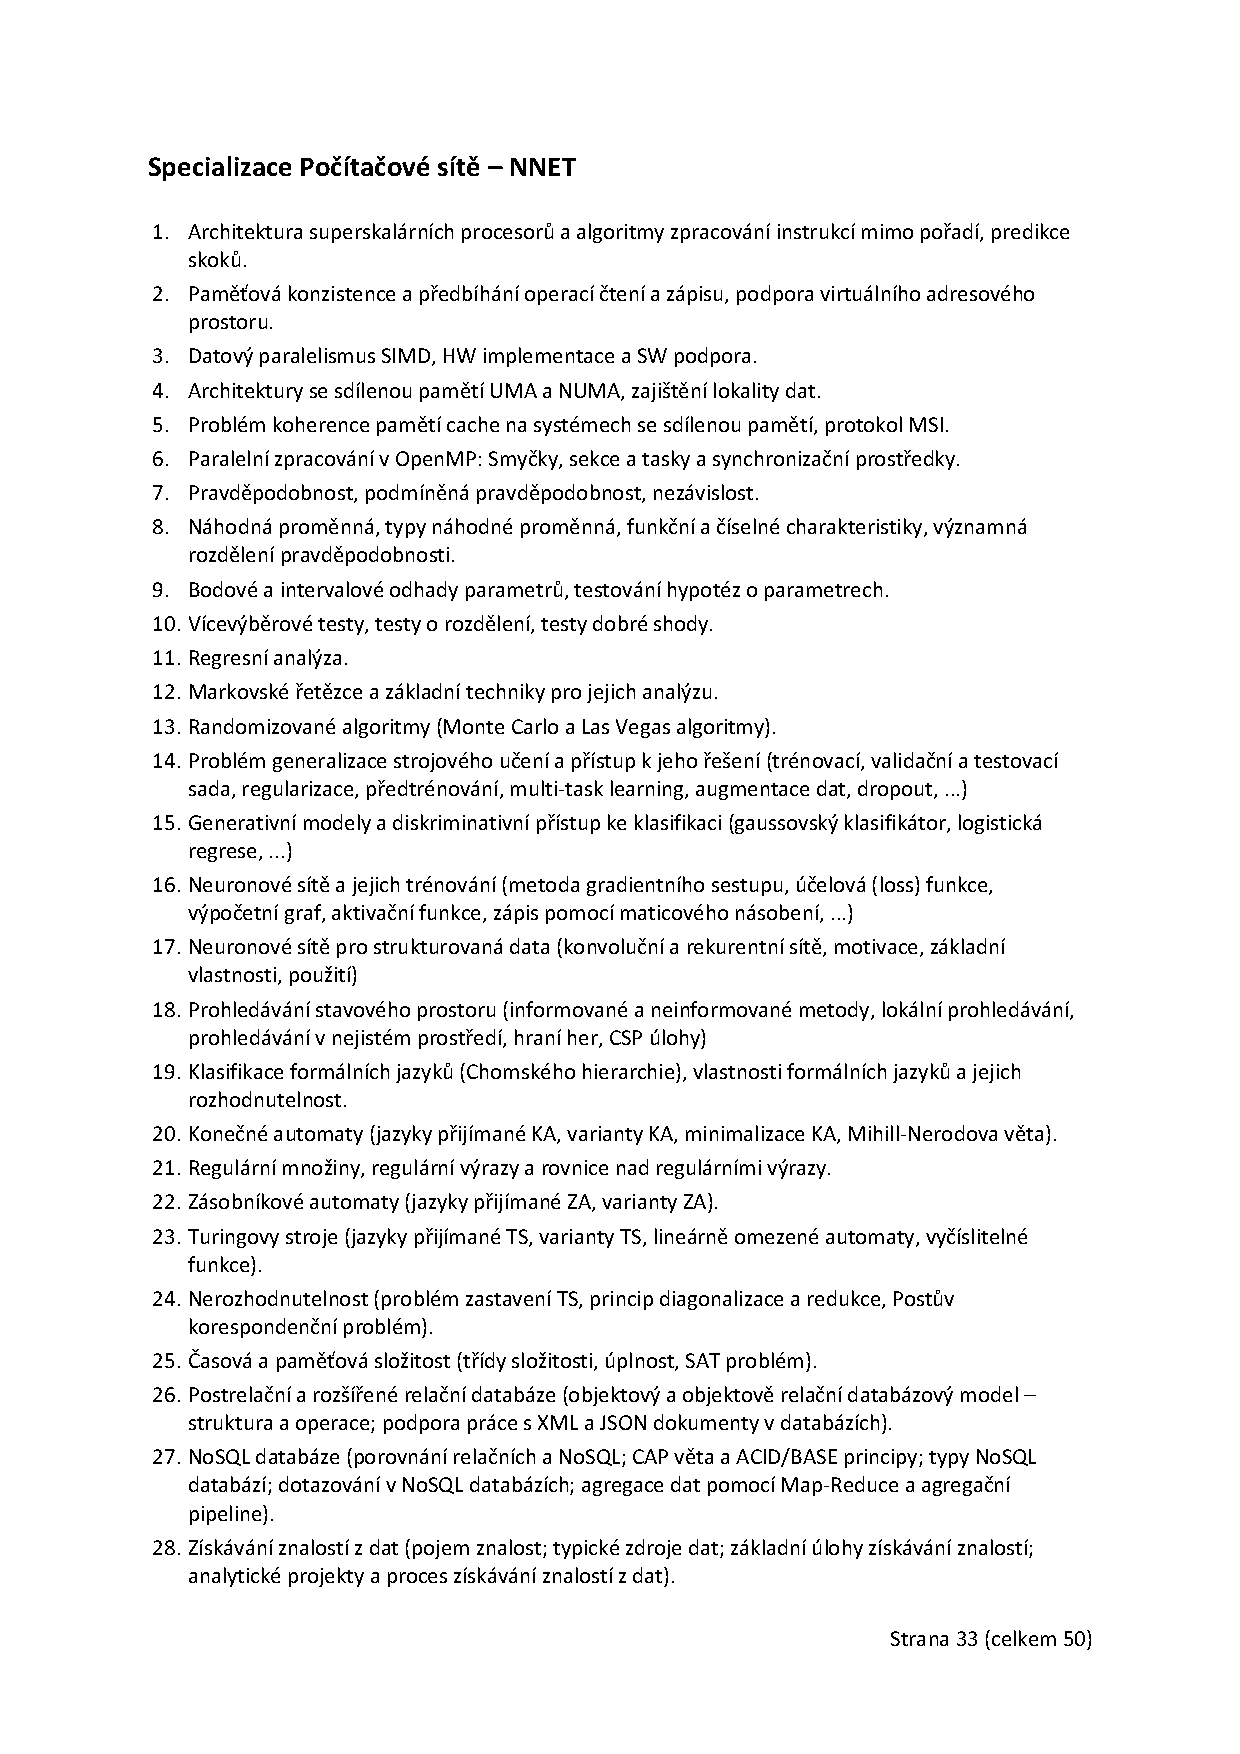
\includepdf[pages=-]{statnicovy_otazky_2022_nnet.pdf}

%%%%%%%%%%%%%%%%%%%%%%%%%%%%%%%%%%%%%%%%%%%%%%%%%%%%%%%%%%%%%%%%%%%%%%%%%%%%%%%%

\tableofcontents
\newpage

%%%%%%%%%%%%%%%%%%%%%%%%%%%%%%%%%%%%%%%%%%%%%%%%%%%%%%%%%%%%%%%%%%%%%%%%%%%%%%%%

% todo
% VUT FIT MITAI
% MSZ 2021/2022
% Author: Vladimir Dusek
% Login: xdusek27

%%%%%%%%%%%%%%%%%%%%%%%%%%%%%%%%%%%%%%%%%%%%%%%%%%%%%%%%%%%%%%%%%%%%%%%%%%%%%%%%

\chapter{Bezdrátové lokální sítě (Wifi, Bluetooth).}

%%%%%%%%%%%%%%%%%%%%%%%%%%%%%%%%%%%%%%%%%%%%%%%%%%%%%%%%%%%%%%%%%%%%%%%%%%%%%%%%

\section{Metadata}

\begin{compactitem}
    \item Předmět: Bezdrátové a mobilní sítě (BMS)
    \item Přednáška:
    \begin{compactitem}
        \item \todo{todo}
    \end{compactitem}
    \item Záznam:
    \begin{compactitem}
        \item \todo{todo}
    \end{compactitem}
\end{compactitem}

%%%%%%%%%%%%%%%%%%%%%%%%%%%%%%%%%%%%%%%%%%%%%%%%%%%%%%%%%%%%%%%%%%%%%%%%%%%%%%%%

\section{Úvod a kontext}

\todo{todo}

\newpage

% VUT FIT MITAI
% MSZ 2021/2022
% Author: Vladimir Dusek
% Login: xdusek27

%%%%%%%%%%%%%%%%%%%%%%%%%%%%%%%%%%%%%%%%%%%%%%%%%%%%%%%%%%%%%%%%%%%%%%%%%%%%%%%%

\chapter{Hledání minimální kostry obyčejného grafu (pojmy, stromy a kostry, Kruskalův algoritmus, Primův algoritmus).}

%%%%%%%%%%%%%%%%%%%%%%%%%%%%%%%%%%%%%%%%%%%%%%%%%%%%%%%%%%%%%%%%%%%%%%%%%%%%%%%%

\section{Metadata}

\begin{compactitem}
    \item Předmět: Grafové algoritmy (GAL)
    \item Přednáška:
    \begin{compactitem}
        \item 5) Stromy, minimální kostry, Jarníkův a Borůvkův algoritmus.
        \item 6) Růst minimální kostry, algoritmy Kruskala a Prima.
    \end{compactitem}
    \item Záznam:
    \begin{compactitem}
        \item 2020-10-22
        \item 2020-10-29
    \end{compactitem}
\end{compactitem}

%%%%%%%%%%%%%%%%%%%%%%%%%%%%%%%%%%%%%%%%%%%%%%%%%%%%%%%%%%%%%%%%%%%%%%%%%%%%%%%%

\section{Úvod a kontext}

\paragraph*{Orientovaný graf} Orientovaný graf je dvojice $G = (V, E)$, kde $V$ je konečná množina uzlů a $E \subseteq V \times V$ je množina hran.

\paragraph*{Neorientovaný graf} Neorientovaný graf je dvojice $G = (V, E)$, kde $V$ je konečná množina uzlů a $E \subseteq \binom{V}{2}$ je množina hran. (Hrana je tedy dvouprvková množina, avšak běžně se držíme stejného značení jako u orientovaných grafů a používáme dvojici.)

\paragraph*{Ohodnocený graf} Ohodnocený graf je takový graf, jehož každá hrana má přiřazenou nějakou hodnotu, typicky definovanou pomocí váhové funkce $w : E \mapsto \mathbb{R}$.

\paragraph*{Podgraf} Graf $G' = (V', E')$ je podgraf grafu $G = (V, E)$ jestliže $V' \subseteq V$ a $E' \subseteq E$.

\paragraph*{Sled} Posloupnost uzlů $\langle v_0, v_1, \dots, v_k \rangle$, kde $(v_{i-1}, v_i) \in E$ pro $i = 1, \dots, k$ se nazývá sled délky $k$ z $v_0$ do $v_k$.

\paragraph*{Uzavřený sled} Sled $\langle v_0, v_1, \dots, v_k \rangle$ se nazývá uzavřený, pokud existuje hrana $(v_0, v_k)$.

\paragraph*{Dosažitelnost} Pokud existuje sled $s$ z uzlu $u$ do uzlu $v$, říkáme, že $v$ je dosažitelný z $u$ sledem $s$, značeno $u \xRightarrow{\text{s}} v$.

\paragraph*{Tah} Tah je sled ve kterém se neopakují hrany.

\paragraph*{Cesta} Cesta je sled ve kterém se neopakují uzly.

\paragraph*{Souvislý graf} Neorientovaný graf se nazývá souvislý, pokud mezi libovolnými dvěma uzly existuje cesta.

\paragraph*{Kružnice} Uzavřená cesta se nazývá kružnice.

\paragraph*{Cyklus} Orientovaná kružnice se nazývá cyklus (první a poslední uzel je shodný).

\paragraph*{Prostý graf} Orientovaný graf bez cyklů se nazývá prostý.

\paragraph*{Acyklický graf} Graf je bez cyklů, resp. kružnic, se nazývá acyklický.

\paragraph*{Strom} Graf, který je souvislý a acyklický, se nazývá strom.

\paragraph*{Kostra} Strom, který tvoří podgraf souvislého grafu na množině všech jeho vrcholů, se nazývá kostra (\textit{spanning tree}).

\paragraph*{Minimální kostra} Nechť $G = (V, E)$ je souvislý neorientovaný graf s váhovou funkcí $w : E \mapsto \mathbb{R}$. Minimální kostra (\textit{MST, minimum spanning tree}) je strom $G' = (V, E')$, kde $E' \subseteq E$ a $$w(E') = \sum_{(u,v) \in T} w(u, v)$$ je minimální ze všech možných alternativních koster.

\paragraph*{Seznam sousedů} Seznam sousedů (\textit{Adj}, \textit{adjacency list}) je reprezentace grafu v paměti. Jde o preferovanou variantu pro řídké grafy~--~kde $m << n^2$. Pro každý uzel máme definovaný seznam jeho sousedů.

\paragraph*{Matice sousednosti} Matice sousednosti (\textit{adjacency matrix}) je reprezentace grafu v paměti. Jde o preferovanou variantu pro husté grafy~--~kde $m$ je skoro $n^2$.

\begin{figure}[H]
    \centering
    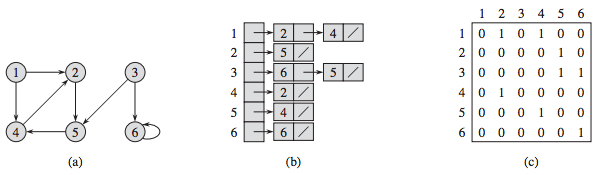
\includegraphics[width=1\linewidth]{gal_1/graph_representations_example.png}
    \caption{Příklad reprezentace grafu pomocí seznamu sousedů a matice sousednosti.}
\end{figure}

%%%%%%%%%%%%%%%%%%%%%%%%%%%%%%%%%%%%%%%%%%%%%%%%%%%%%%%%%%%%%%%%%%%%%%%%%%%%%%%%

\section{Generický algoritmus}

Hledání minimální kostry je problém, který lze řešit algoritmy, které spadají do kategorie tzv. hladových (\textit{greedy}) deterministických algoritmů. Spočívají v tom, že průběžně odhadují kostru přidáváním dalších hran a nikdy se nemusejí vracet (neprovádí se \textit{backtracking}). Generický algoritmus tvoří jakousi základní kostru pro další, už konkrétní, algoritmy.

\paragraph*{Řez} Nechť $G = (V, E)$ je graf. Řez grafu $G$ je dvojice $(S, V - S)$, kde $\emptyset \subseteq S \subseteq V$.

\paragraph*{Křížení} Hrana $(u, v) \in E$ kříží řez $(S, V - S)$, pokud jeden její konec je v $S$ a druhý v $V - S$.

\paragraph*{Respektování} Nechť $A \subseteq E$ je množina hran. Řez $(S, V - S)$ respektuje množinu hran $A$, pokud žádná hrana v $A$ nekříží řez $(S, V - S)$.

\paragraph*{Lehkost} Nechť $(S, V - S)$ je řez a $B$ je množina hran, která ho kříží. Hrana z množiny $B$ s nejmenší hodnotou se nazývá lehká.

\paragraph*{Bezpečnost} Nechť $G = (V, E)$ je souvislý neorientovaný graf s reálnou váhovou funkcí $w$. Nechť $A \subseteq E$ je součástí nějaké minimální kostry $G$. Nechť $(S, V - S)$ je řez, který respektuje $A$. Nechť $(u, v)$ je lehká hrana křížící $(S, V - S)$. Pak hrana $(u, v)$ je bezpečná pro $A$.

\bigskip\noindent\begin{minipage}{\linewidth}
\begin{lstlisting}[language=Python, caption={Generický algoritmus. Před každou iterací algoritmu je množina $A$ podmnožinou nějaké minimální kostry. Hrana $(u,v) \in E$ je bezpečná pro $A$, pokud $A \cup \{(u, v)\}$ je podmnožinou nějaké minimální kostry.}]
def generic_mst(G):
    # G je graf
    A = {} # A je mnozina hran rozpracovane minimalni kostry
    while netvori_kostru(A, G):
        for hrana in G.E:
            if je_bezpecna(A, hrana):
                A += {hrana}
    return A
\end{lstlisting}
\end{minipage}

\begin{figure}[H]
    \centering
    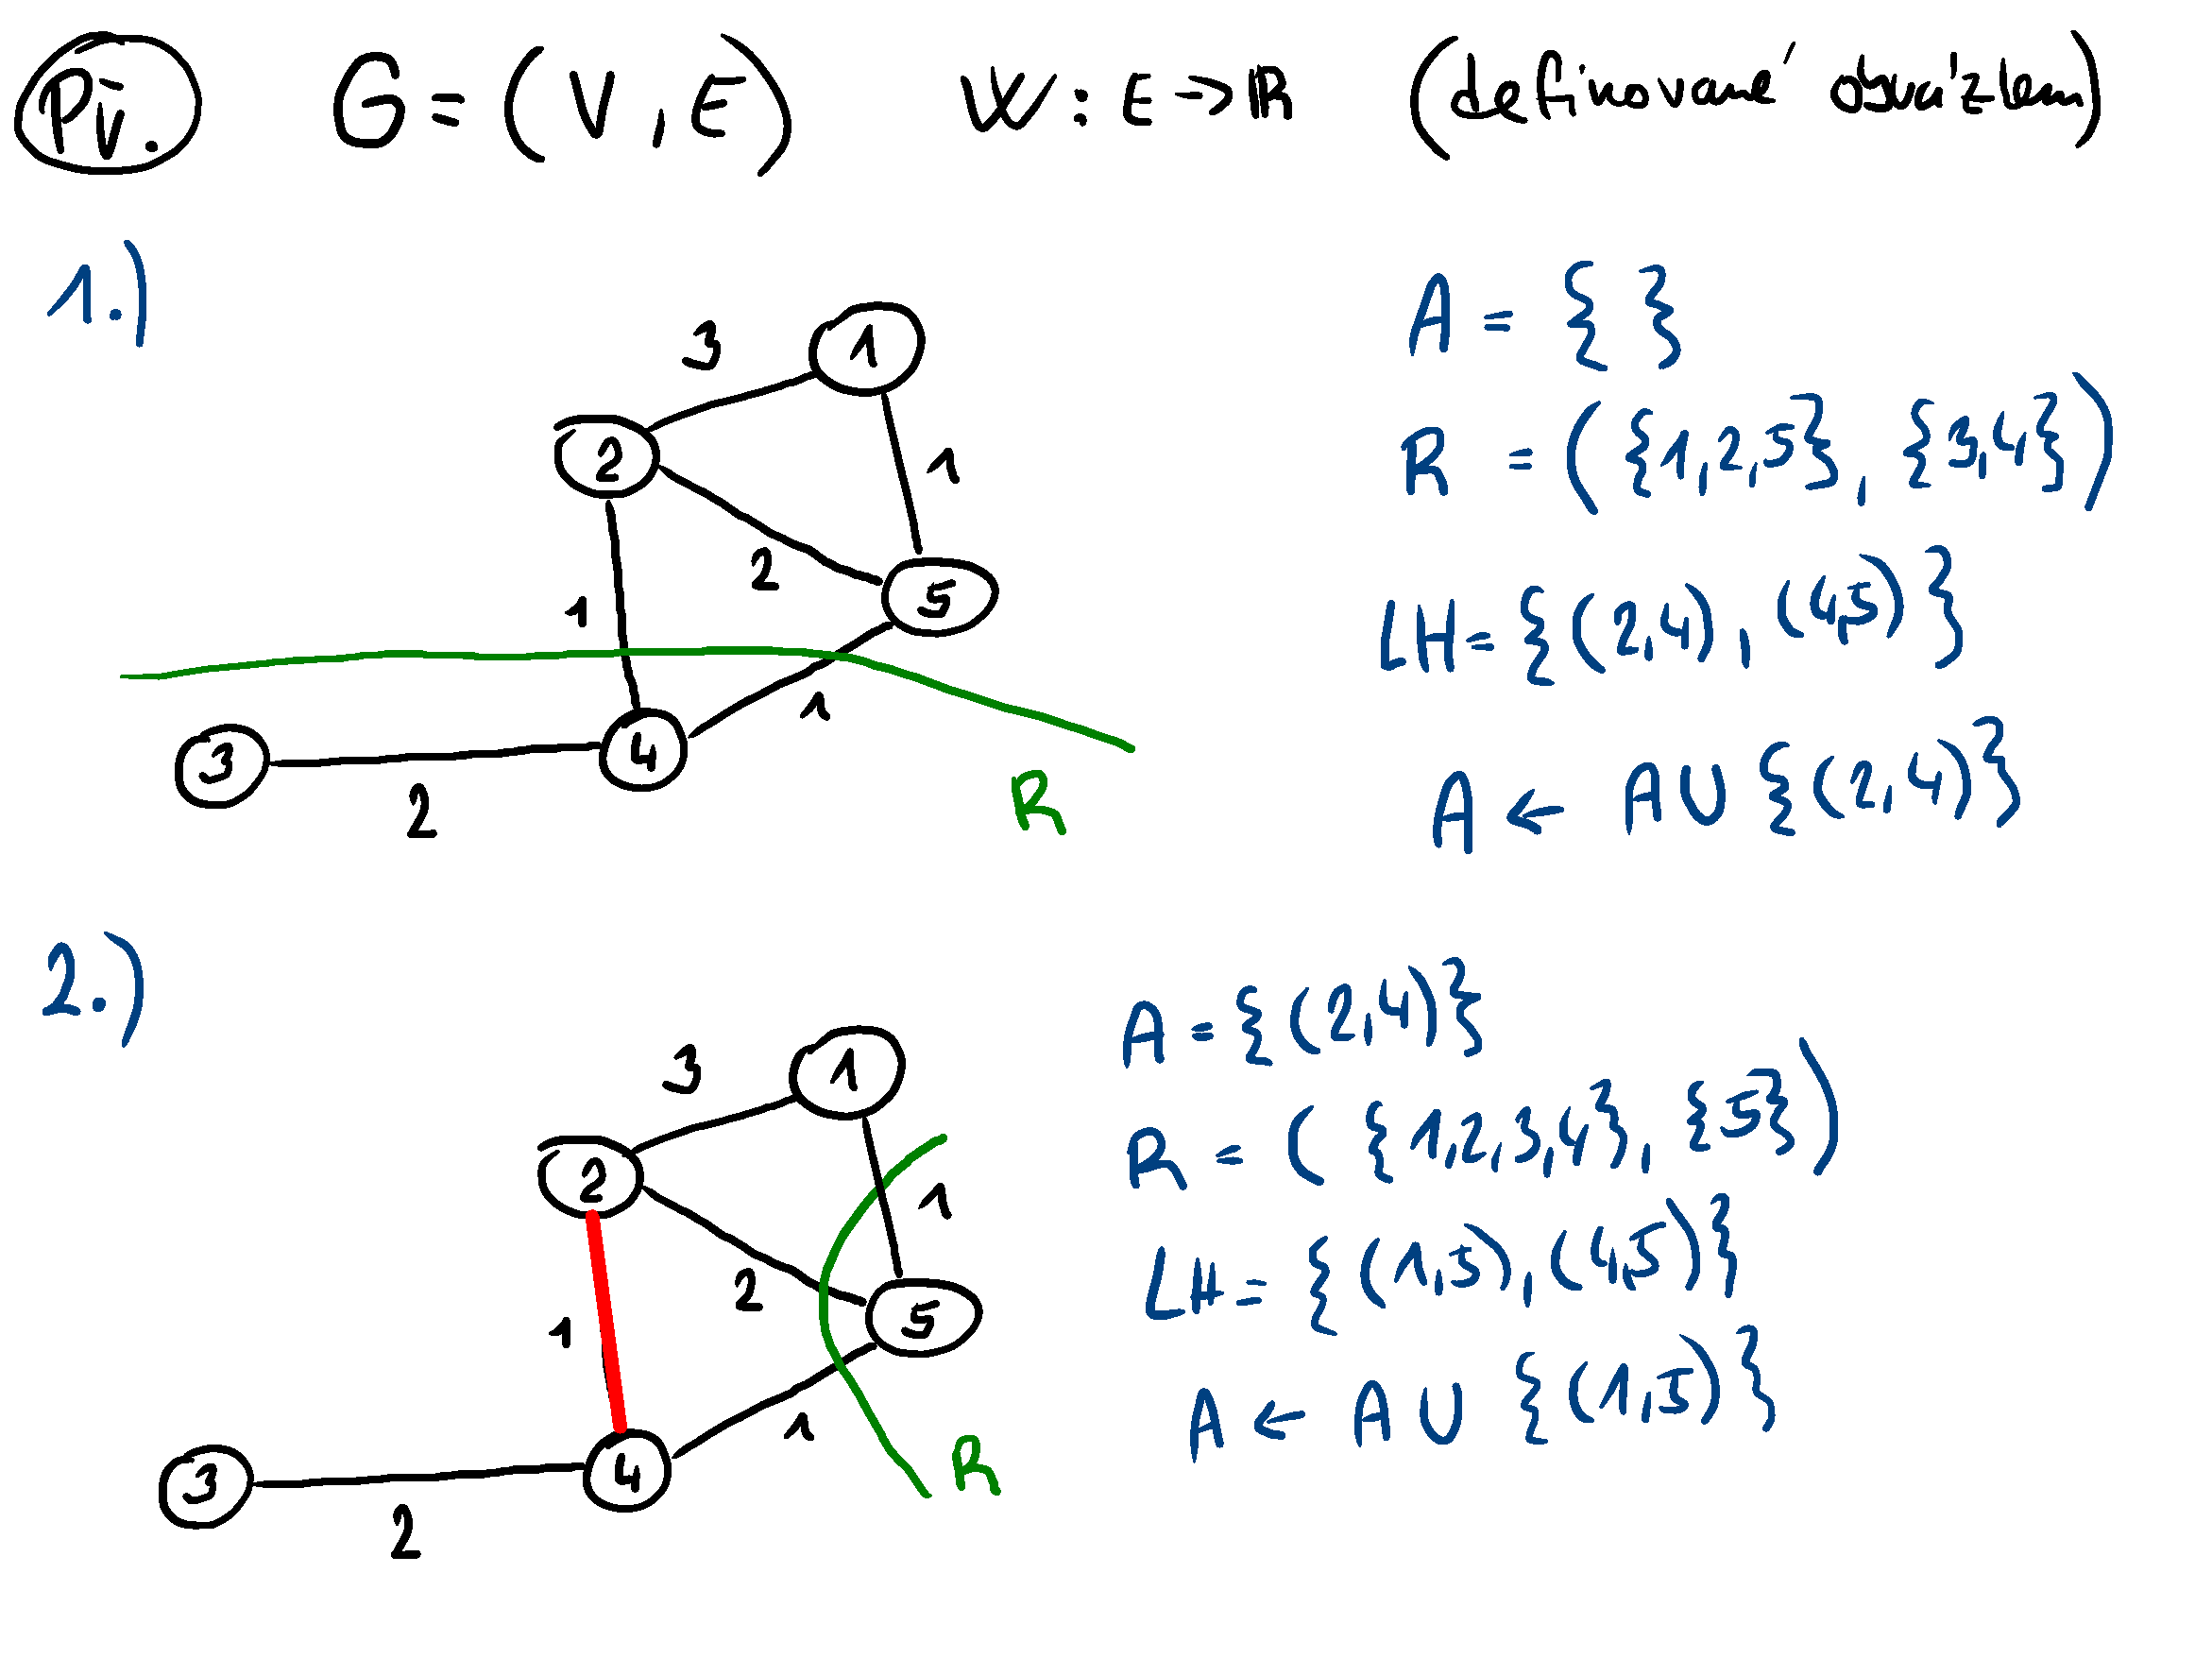
\includegraphics[width=0.9\linewidth]{gal_1/03-minimalni-kostry-6.pdf}
    \caption{Příklad, část 1.}
\end{figure}

\begin{figure}[H]
    \centering
    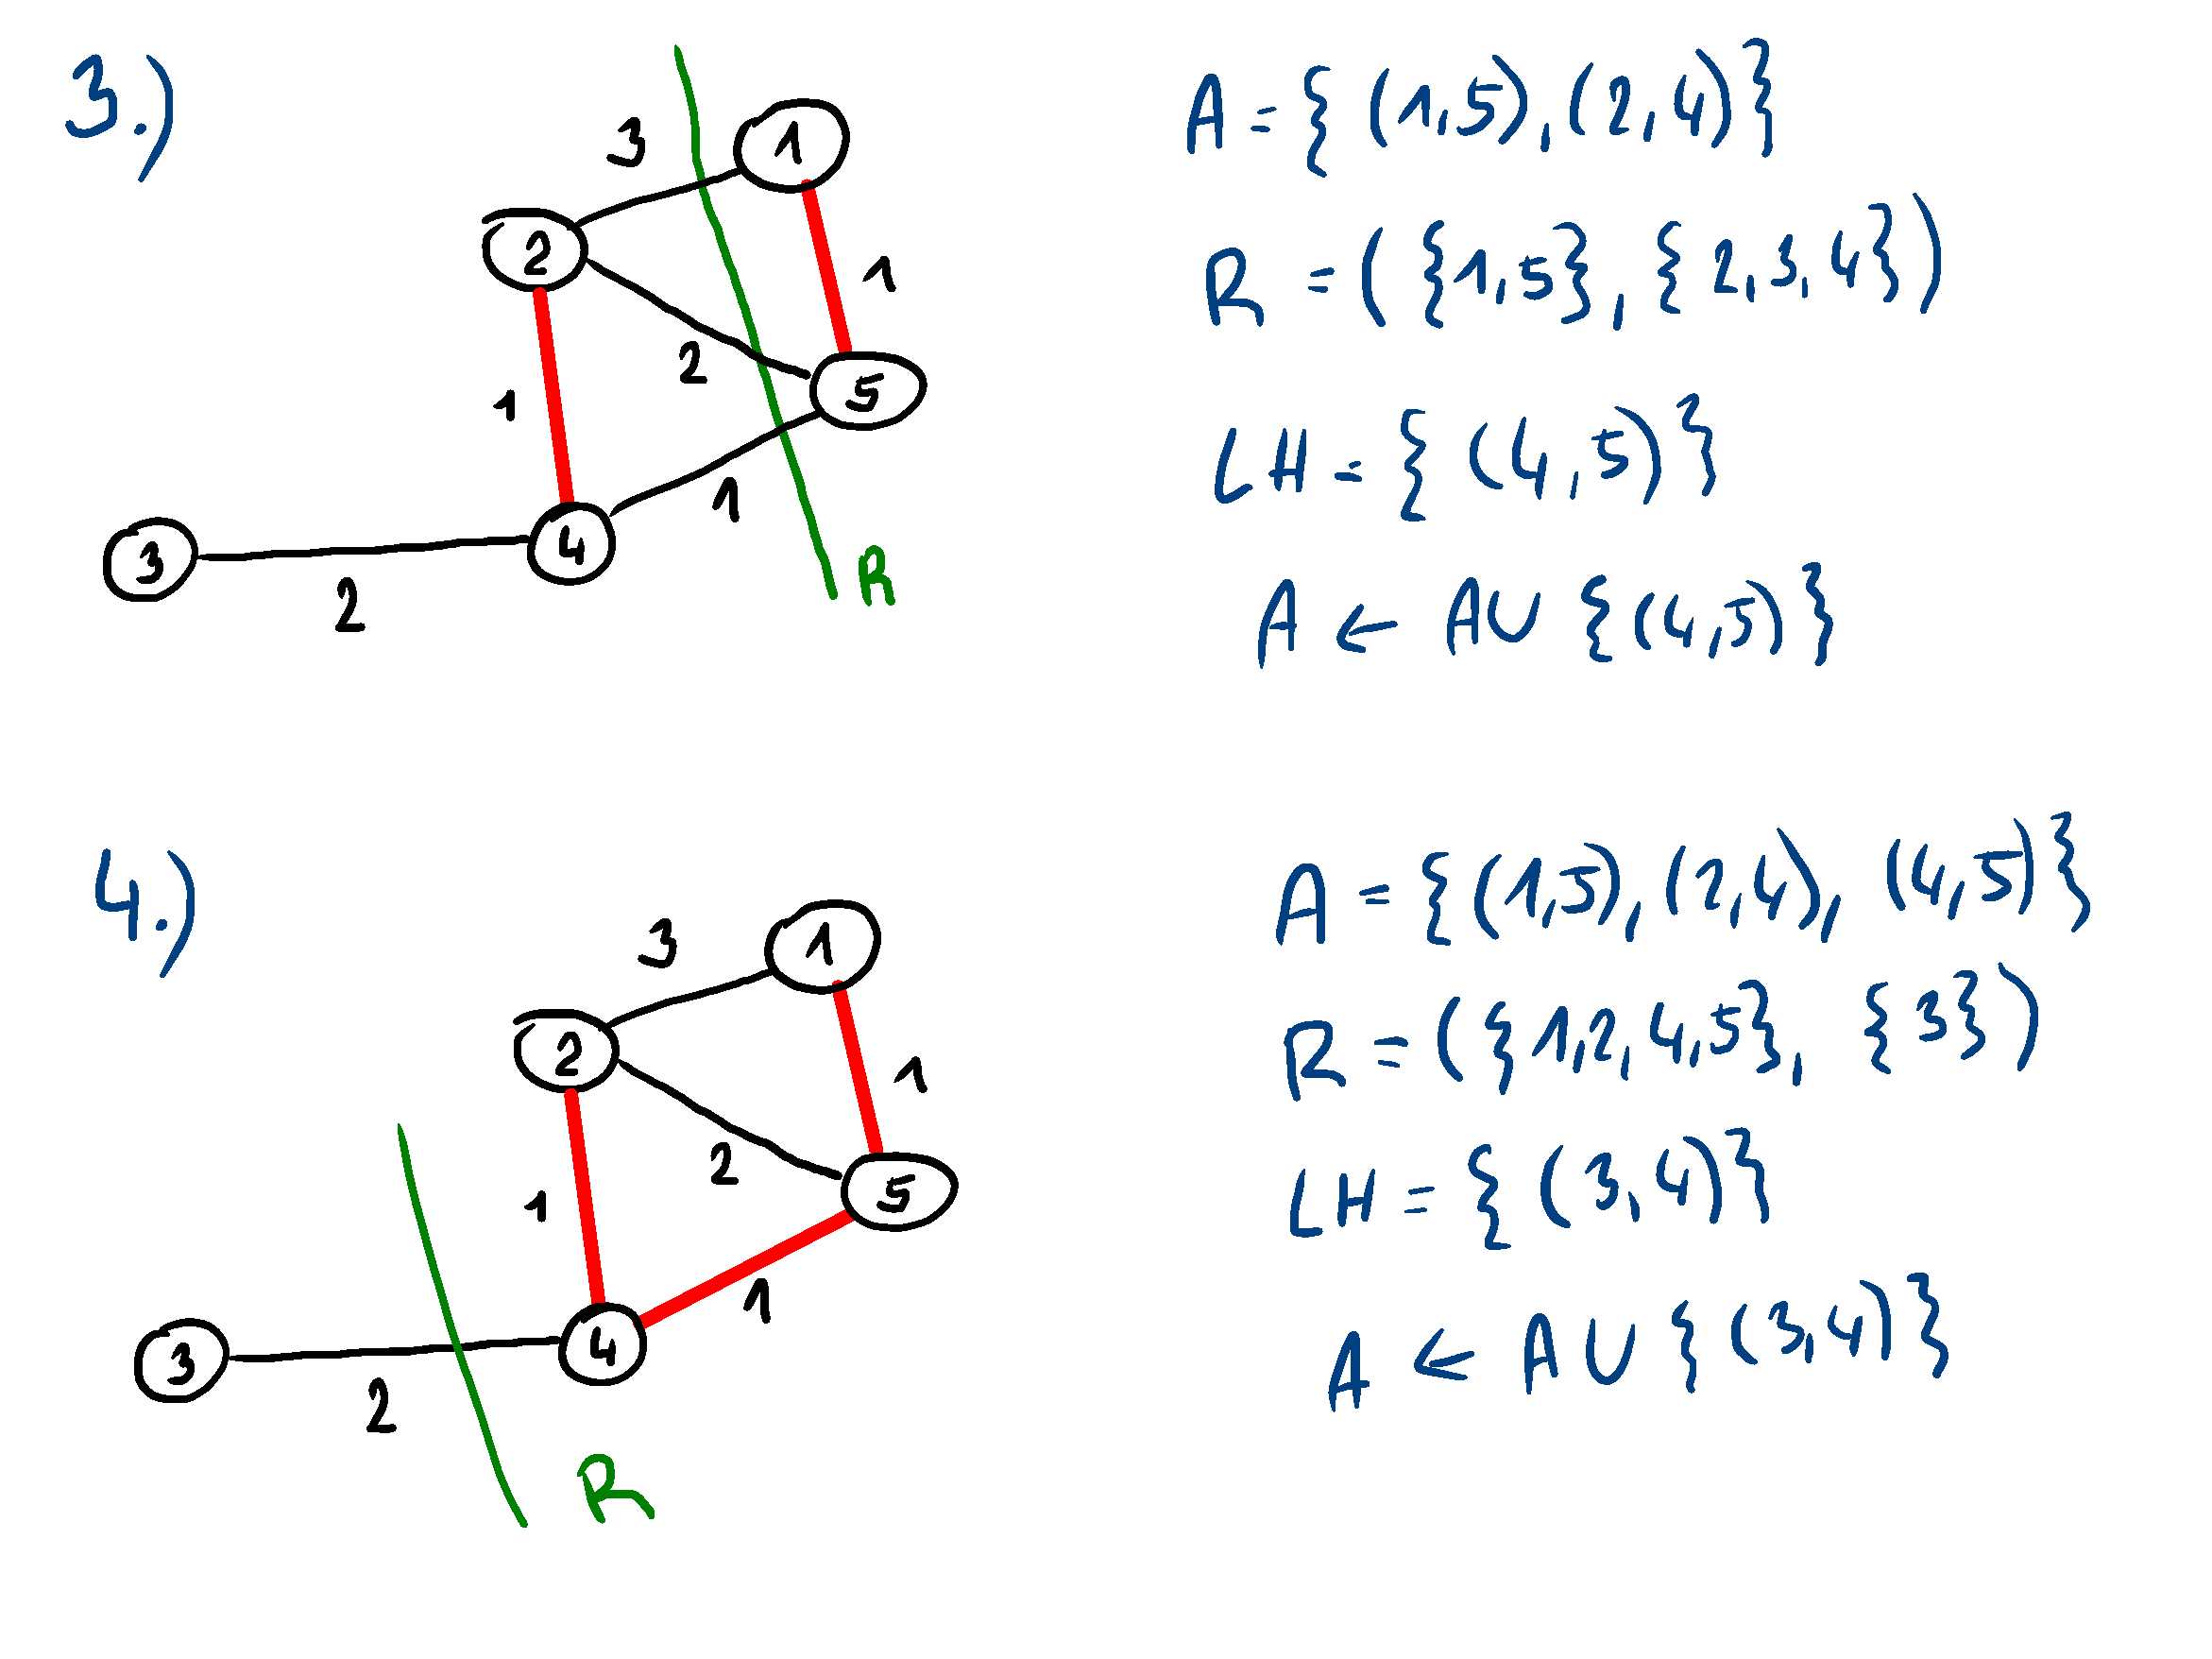
\includegraphics[width=0.9\linewidth]{gal_1/03-minimalni-kostry-7.pdf}
    \caption{Příklad, část 2.}
\end{figure}

\begin{figure}[H]
    \centering
    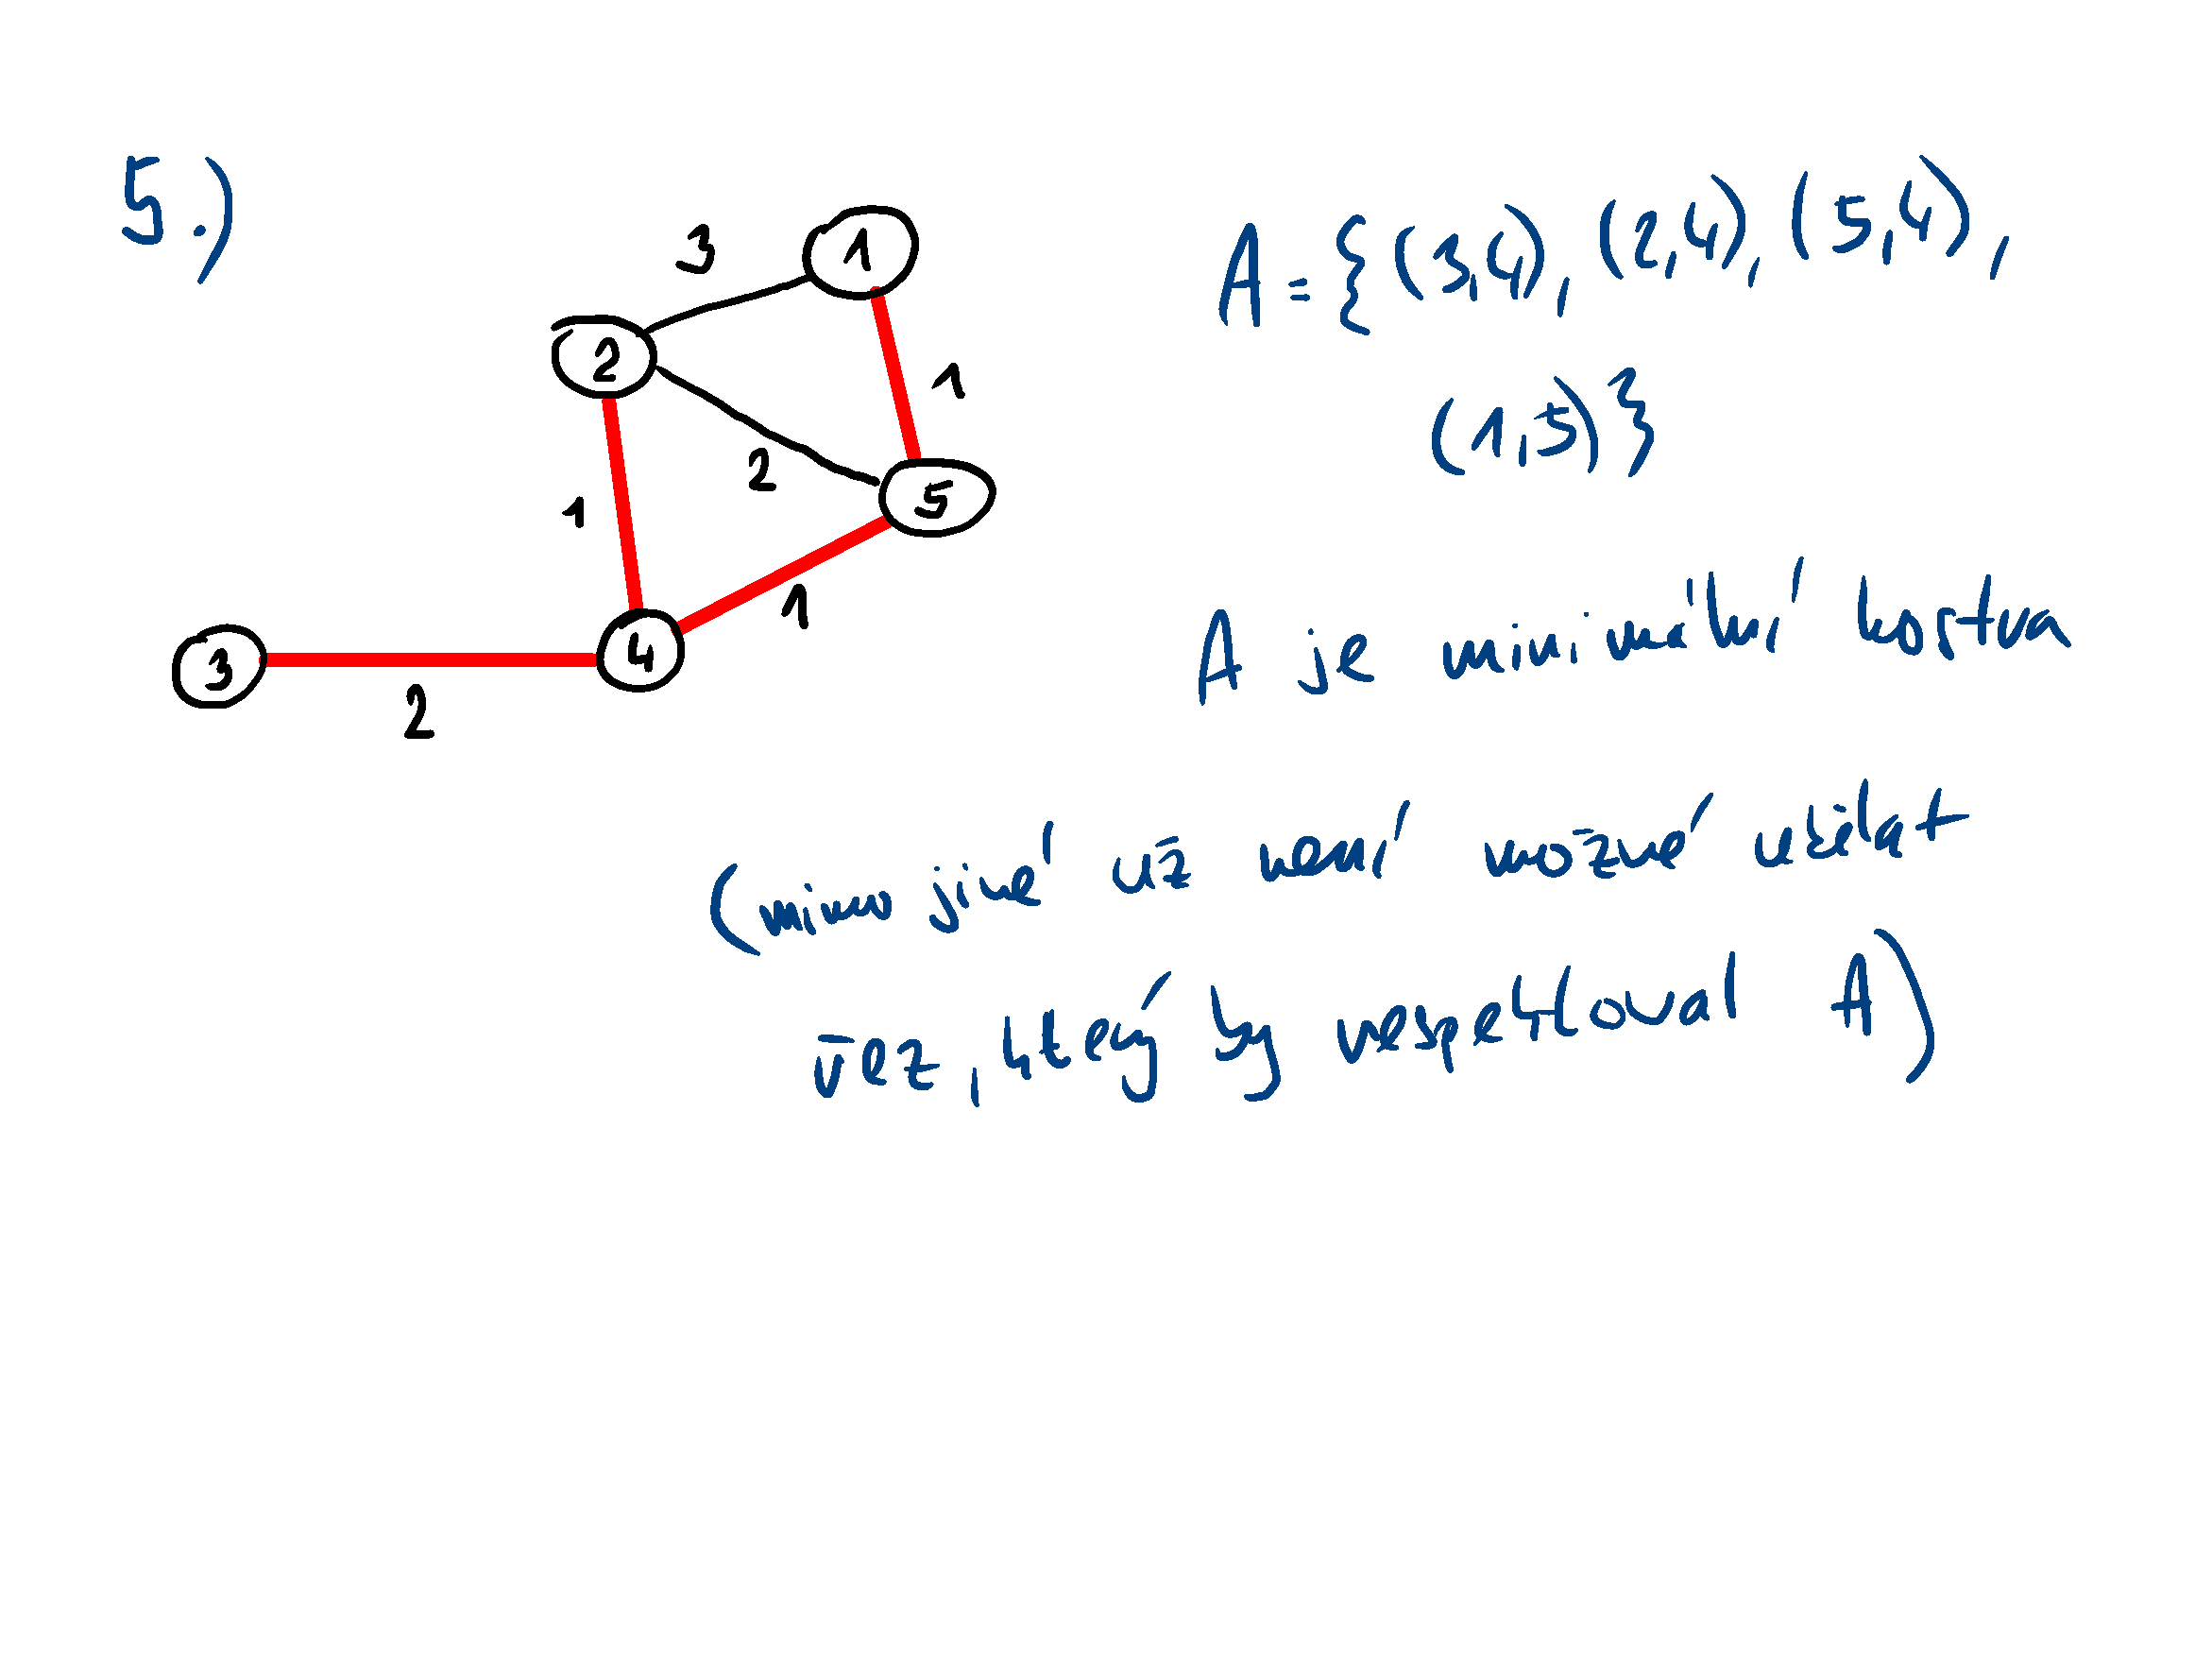
\includegraphics[width=0.9\linewidth]{gal_1/03-minimalni-kostry-8.pdf}
    \caption{Příklad, část 3.}
\end{figure}

%%%%%%%%%%%%%%%%%%%%%%%%%%%%%%%%%%%%%%%%%%%%%%%%%%%%%%%%%%%%%%%%%%%%%%%%%%%%%%%%

\section{Kruskalův algoritmus}

Kruskalův a Primův algoritmus se liší v tom, jakým způsobem vybírají bezpečnou hranu. Kruskalův algoritmus nahlíží na $A$ jako na les a hledá hranu s nejmenším ohodnocením, která spojuje stromy v lese. Na konci je $A$ jeden strom.

\bigskip\noindent\begin{minipage}{\linewidth}
\begin{lstlisting}[language=Python, caption={Kruskalův algoritmus. Funkce \texttt{make\_set(v)} vytvoří množinu obsahující $v$, \texttt{find\_set(v)} vrátí reprezentanta množiny ve které se nachází $v$, \texttt{union(u, v)} sjednotí dvě množiny obsahující $u$ a $v$.}]
def kruskal_mst(G):
    # G je graf

    # inicializace, kazdy uzel je ve sve mnozine
    A = {} # A je mnozina hran rozpracovane minimalni kostry
    for v in G.V:
        make_set(v)

    # seradit vzestupne podle w
    E = sort(G.E, G.w)

    for (u, v) in E:
        if find_set(u) != find_set(v):
            A += {(u, v)}
            union(u, v)

    return A
\end{lstlisting}
\end{minipage}

\subsection*{Složitost}

\begin{compactitem}
    \item Řádek 5 -- $O(1)$
    \item Řádek 6-7 -- $n$-krát složitost $make\_set$ ($n$ je počet uzlů).
    \item Řádek 10 -- $O(m \cdot \log(m))$ ($m$ je počet hran).
    \item Řádky 12-15 -- Závisí na implementaci $find\_set$ a $union$.
    \begin{compactitem}
        \item Při implementaci seznamem s heuristickou celkem: $O(m + n \cdot \log(n))$.
        \item Při stromové implementaci s váhami a zkratkami celkem: $O((m+n) \cdot \alpha(n))$. Kde $\alpha$ je velmi pomalu rostoucí funkce ($\alpha \leq 4$).
    \end{compactitem}
    \item Pro souvislý graf platí $m > n$. Proto množinové operace stojí $O(m \cdot \alpha(n))$. Jelikož $\alpha(n) = O(\log(n)) = O(\log(m))$, tak celková složitost je $O(m \cdot \log(m))$.
    \item Dále platí $m < n^2$, pak $\log(m) = O(\log(n))$, proto celkem: $O(m \cdot \log(n))$.
\end{compactitem}

\subsection*{Příklad}

\begin{figure}[H]
    \centering
    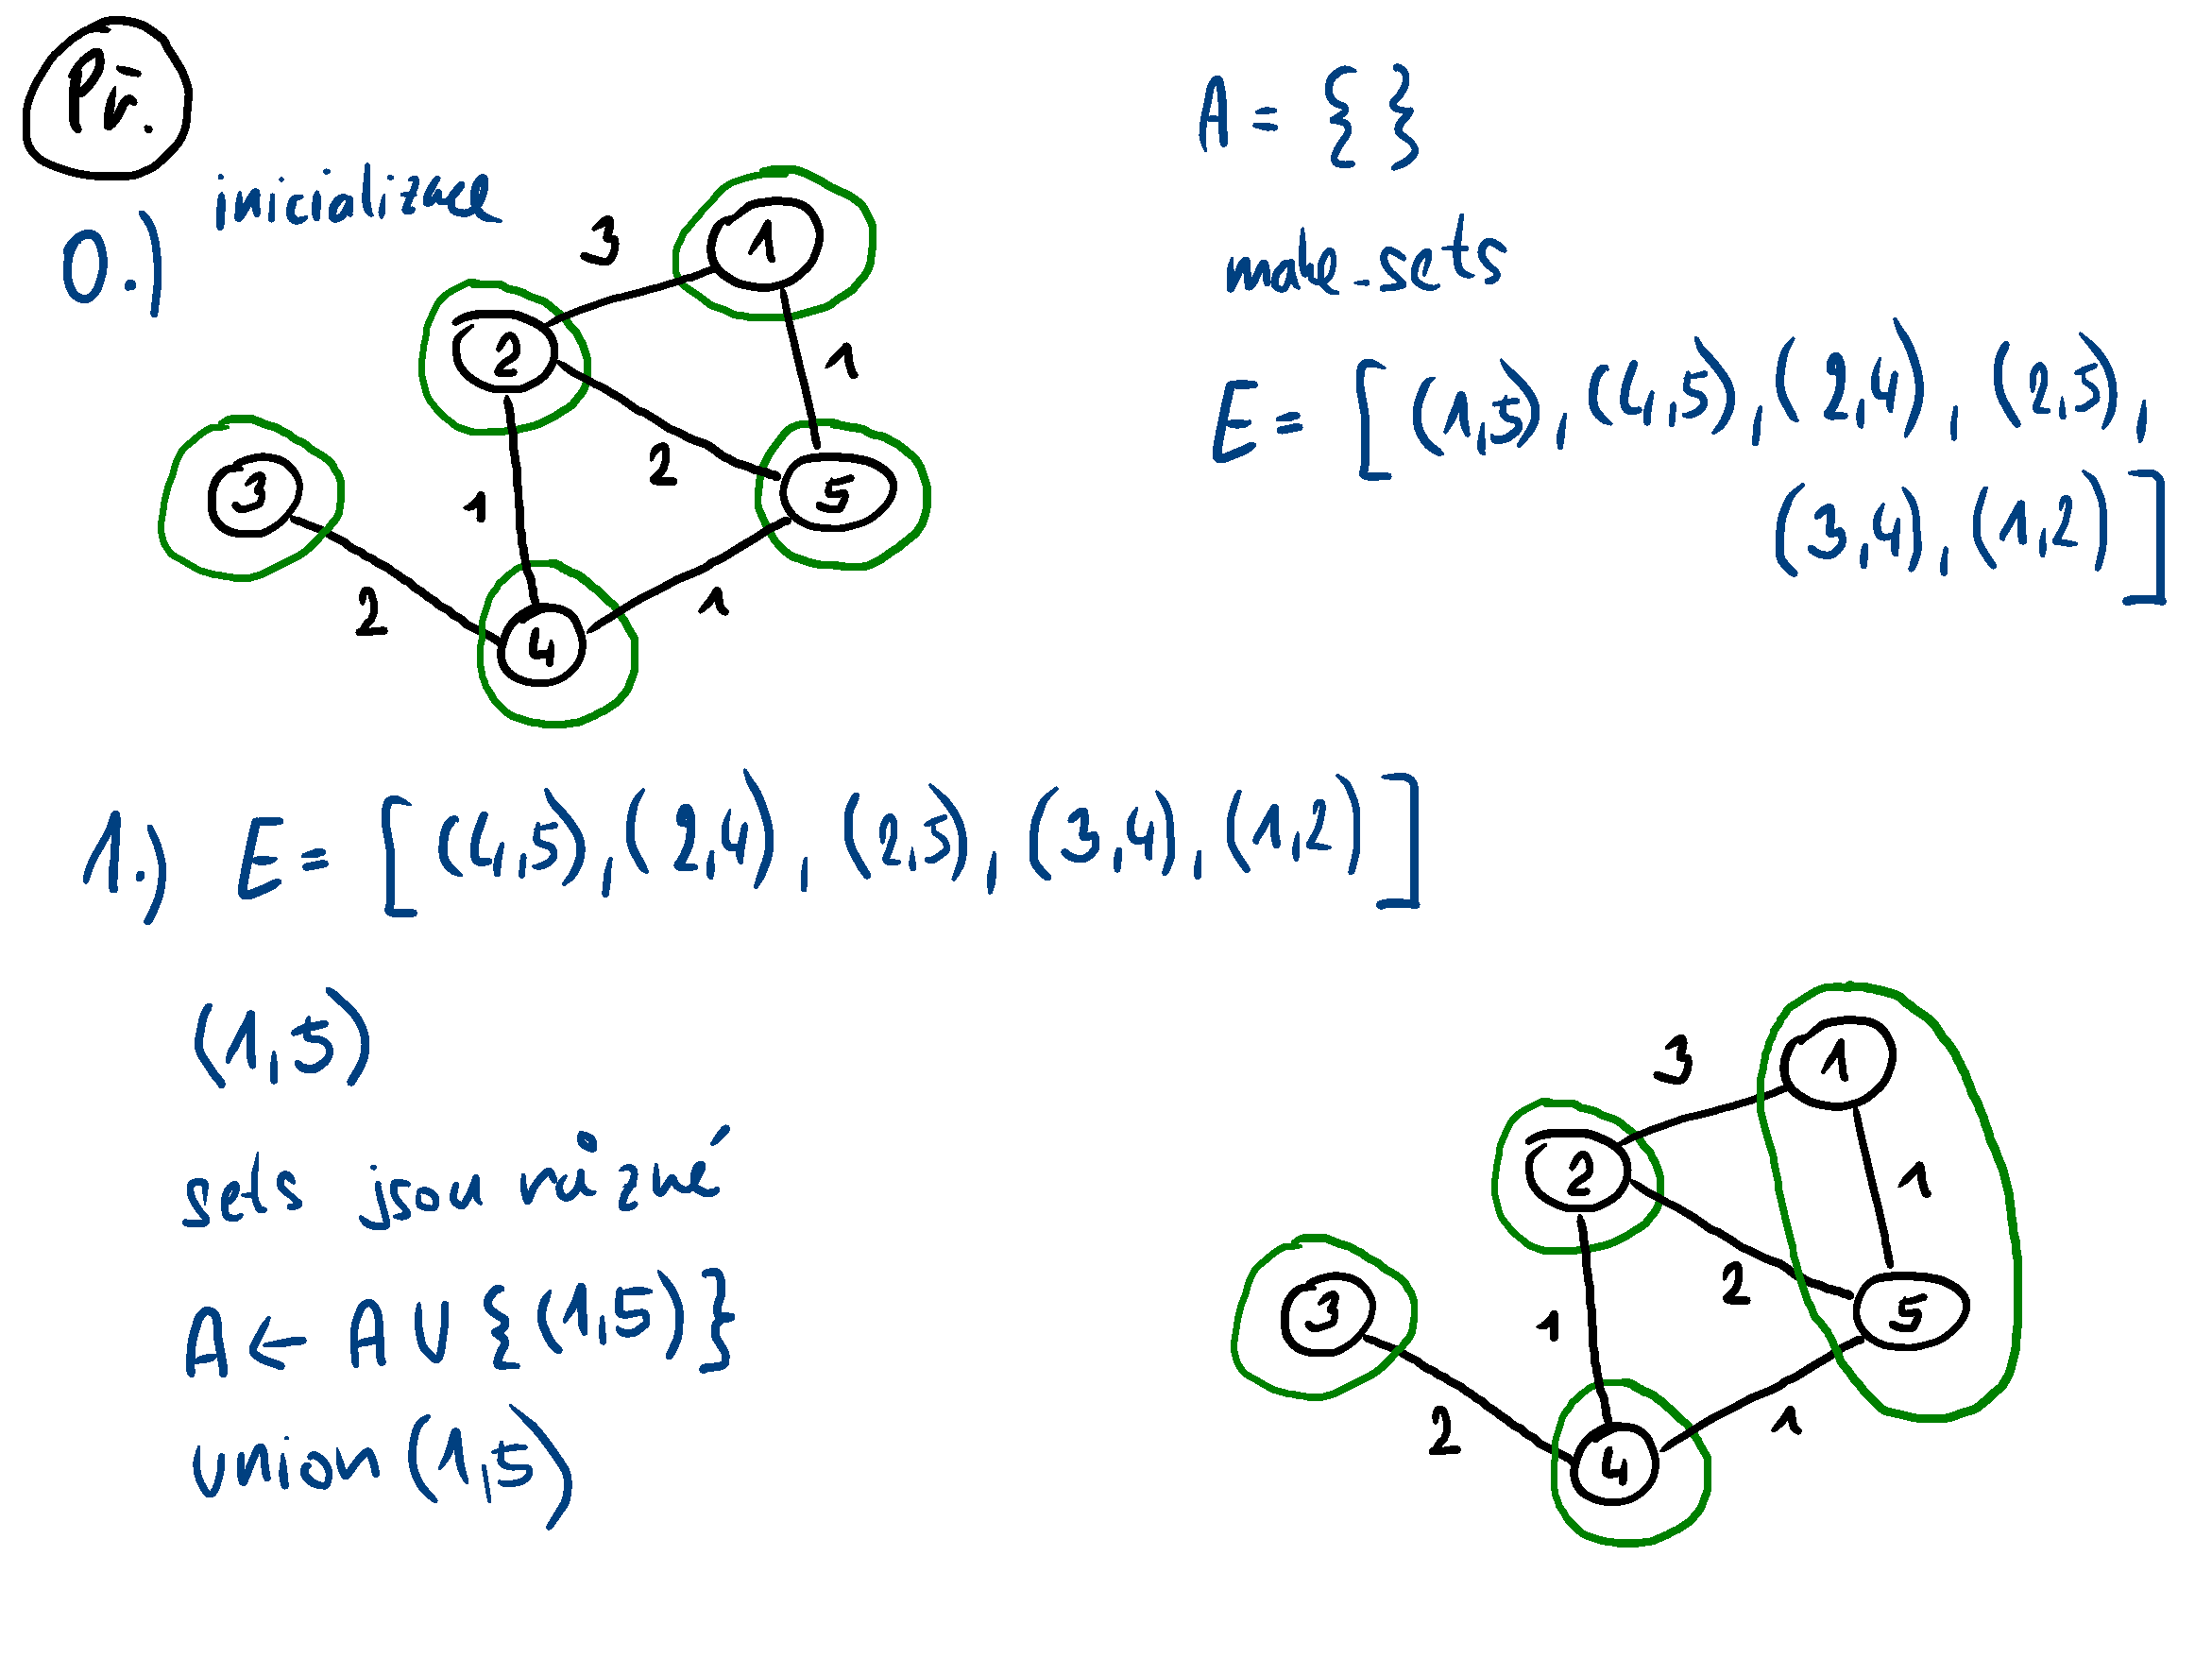
\includegraphics[width=0.9\linewidth]{gal_1/03-minimalni-kostry-11.pdf}
    \caption{Příklad, část 1.}
\end{figure}

\begin{figure}[H]
    \centering
    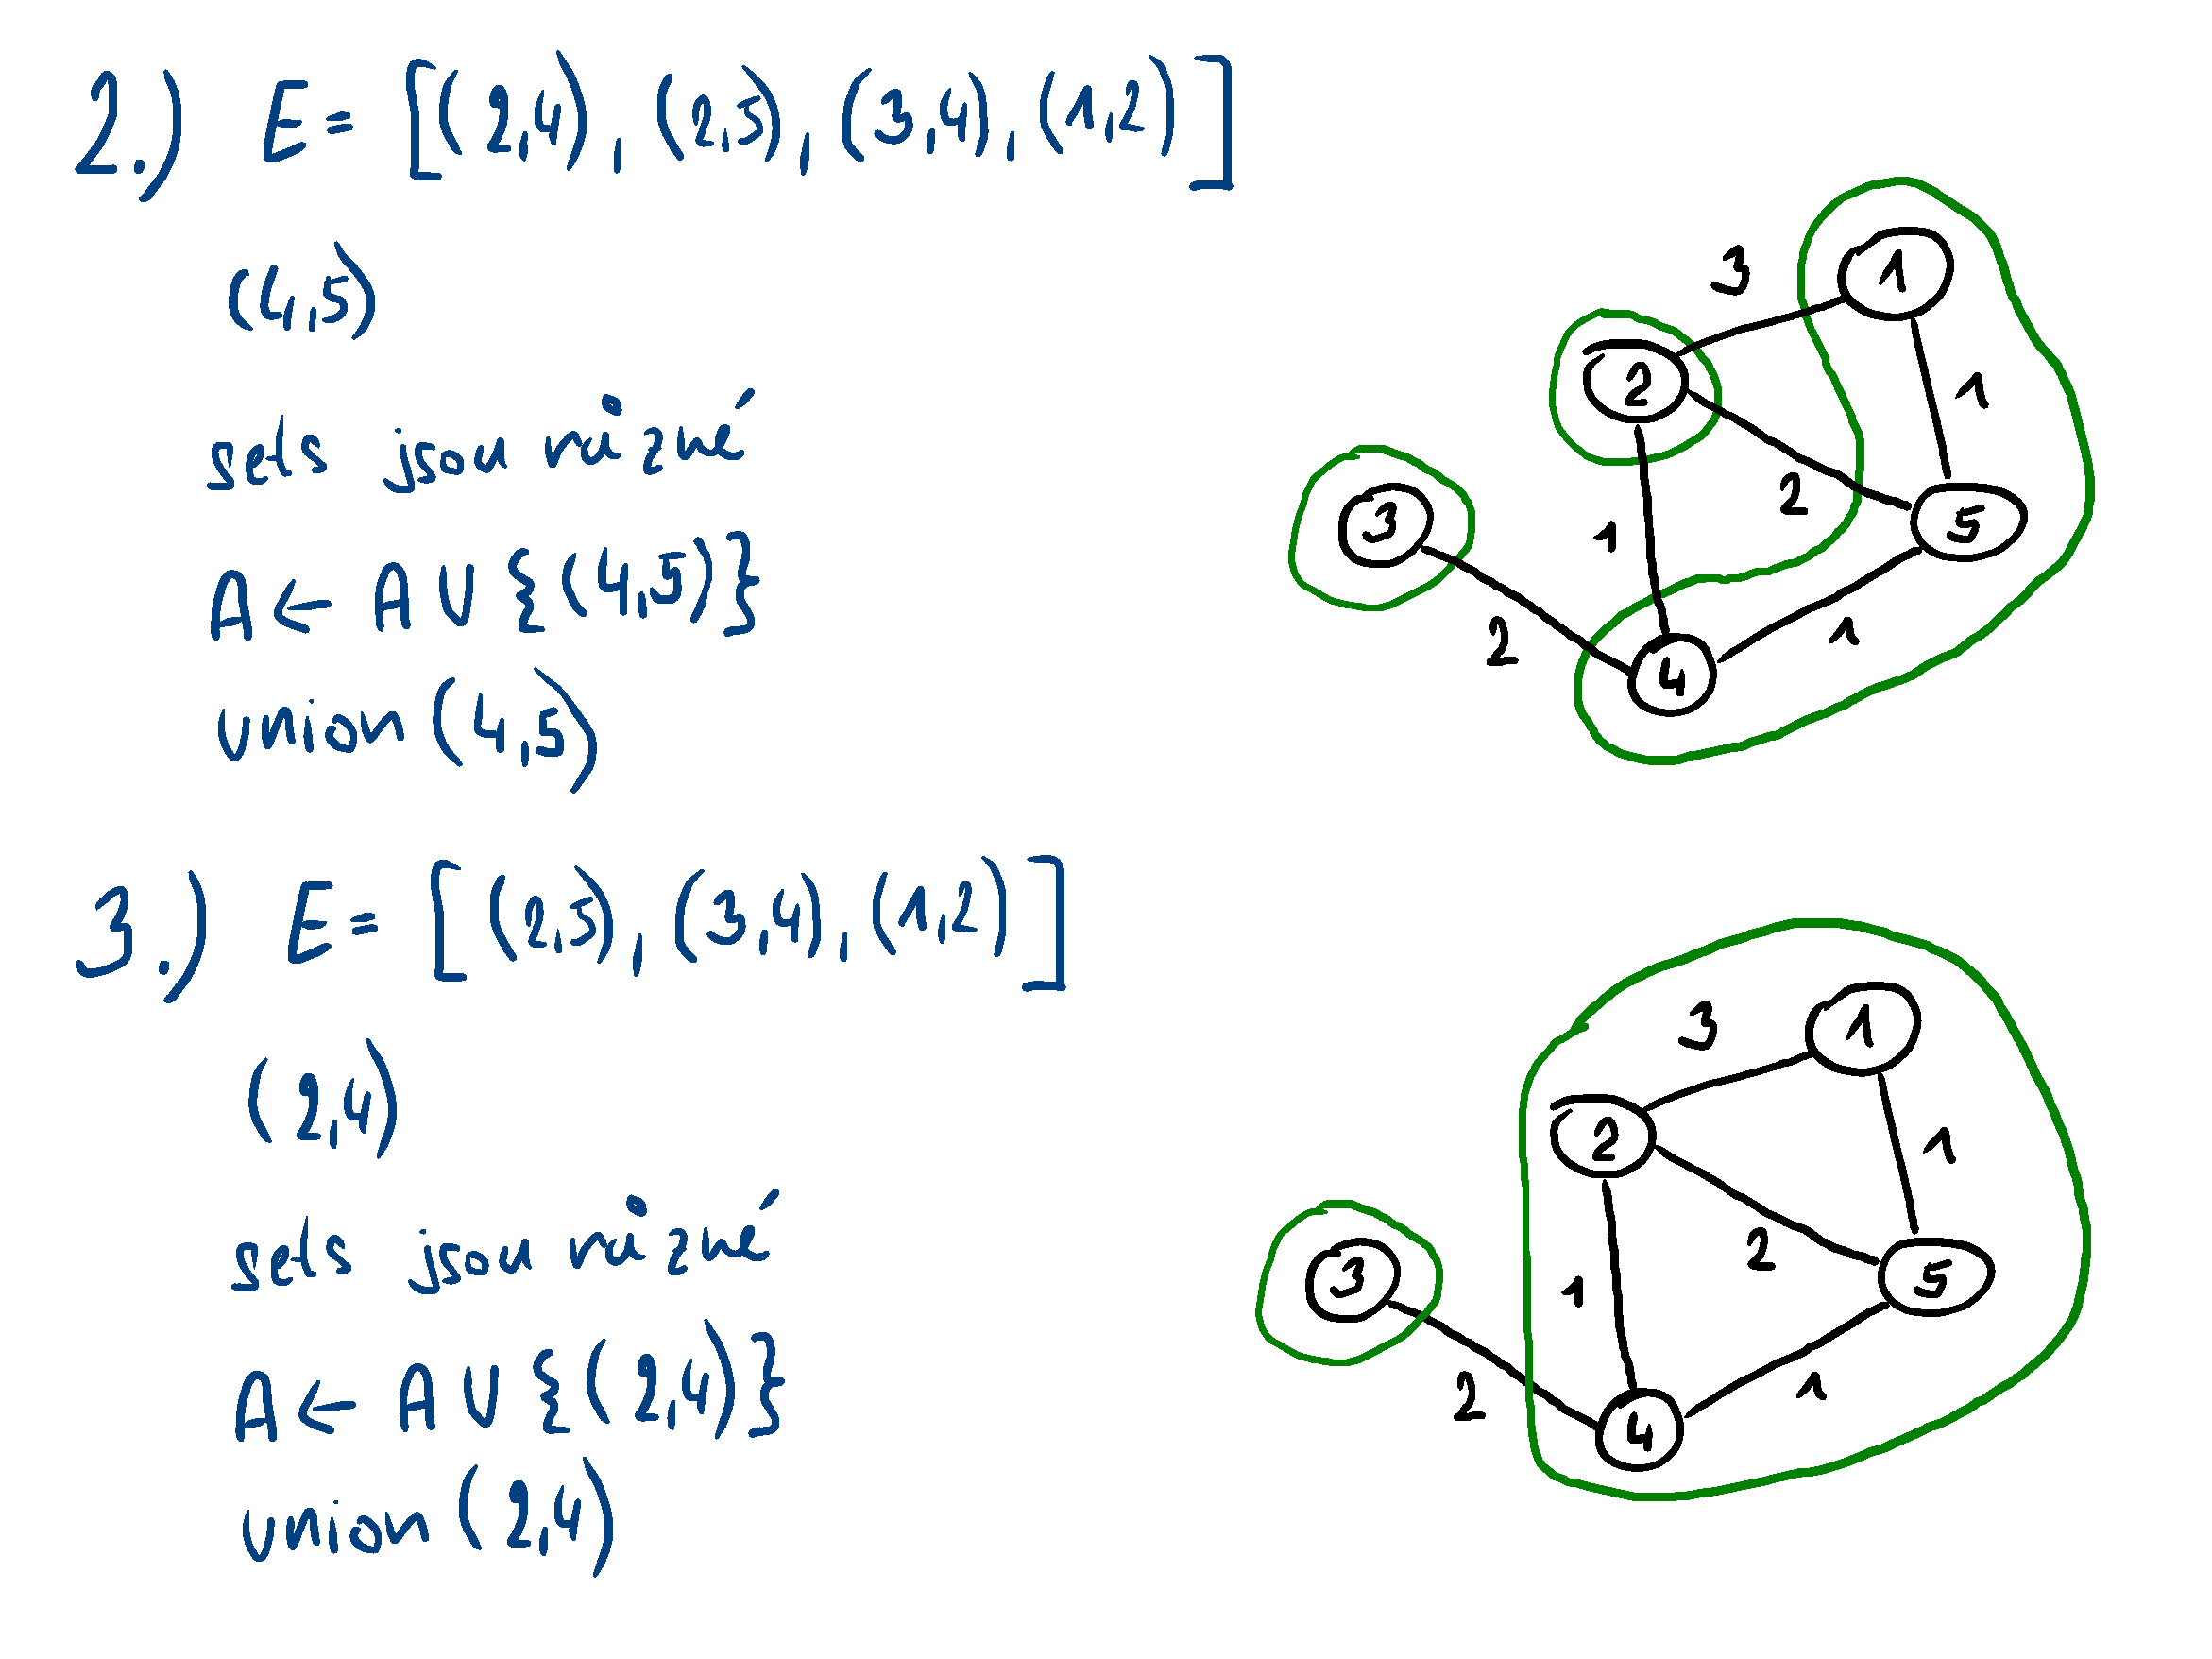
\includegraphics[width=0.9\linewidth]{gal_1/03-minimalni-kostry-12.pdf}
    \caption{Příklad, část 2.}
\end{figure}

\begin{figure}[H]
    \centering
    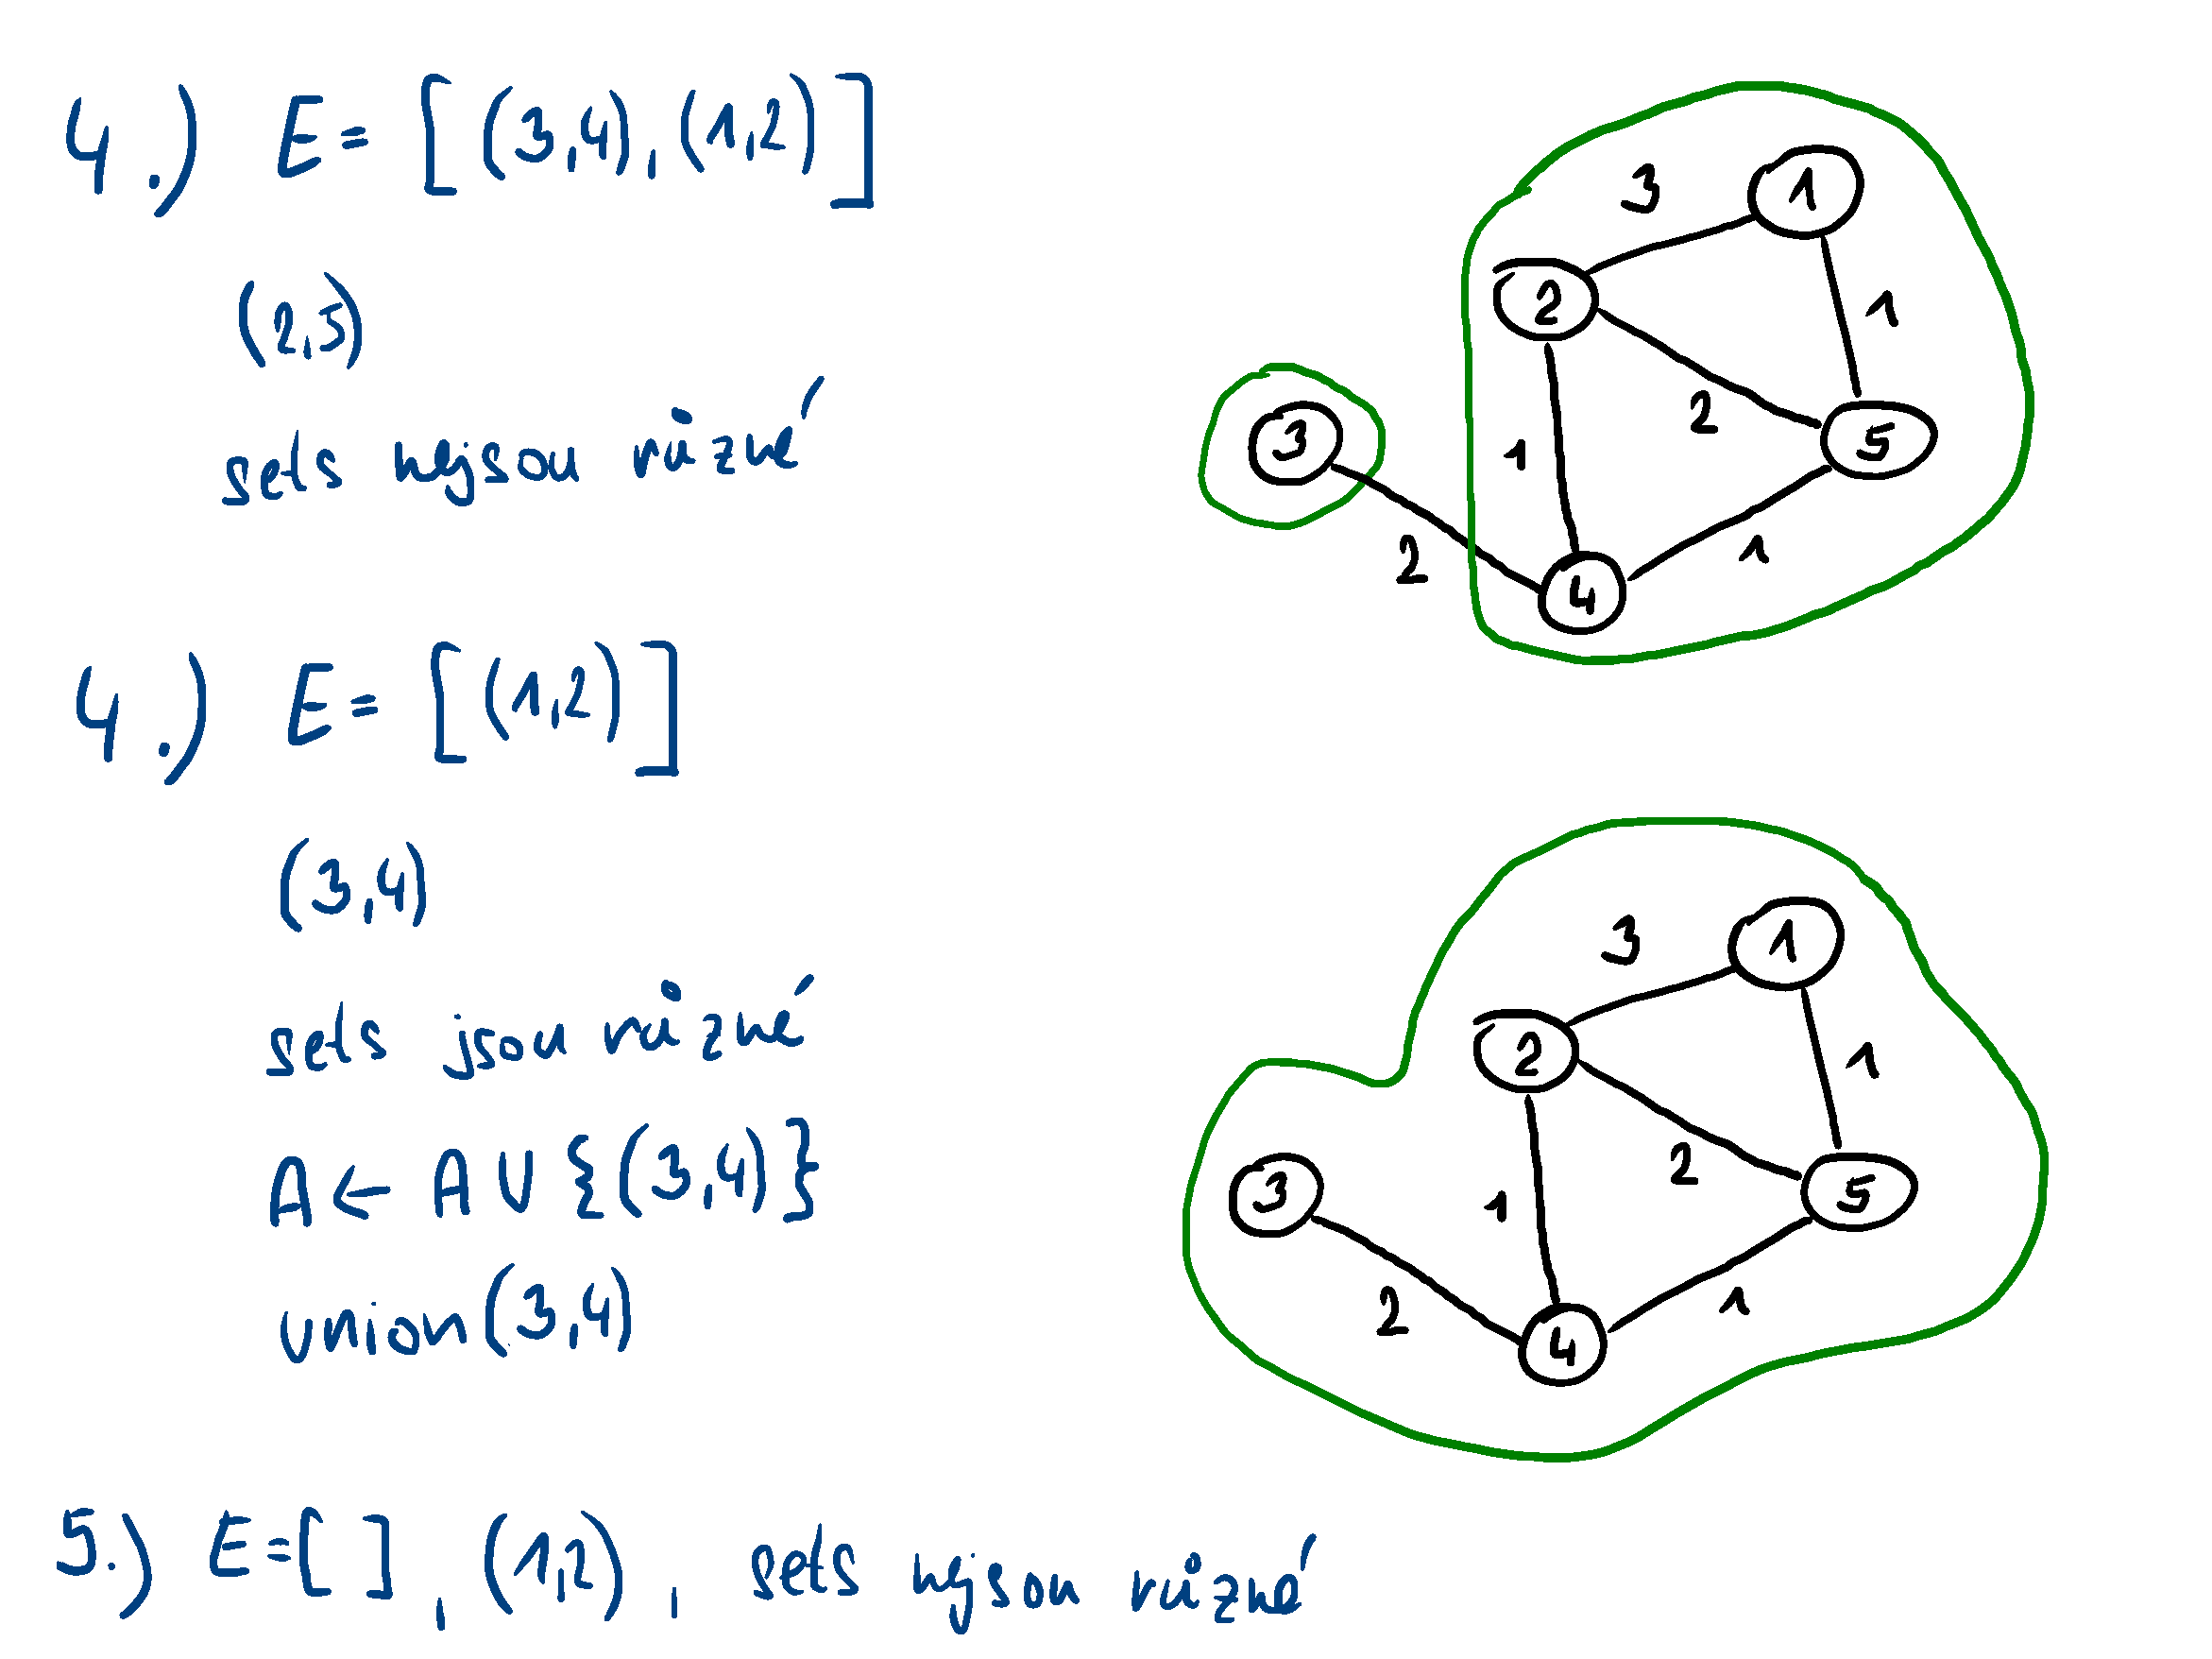
\includegraphics[width=0.9\linewidth]{gal_1/03-minimalni-kostry-13.pdf}
    \caption{Příklad, část 3.}
\end{figure}

%%%%%%%%%%%%%%%%%%%%%%%%%%%%%%%%%%%%%%%%%%%%%%%%%%%%%%%%%%%%%%%%%%%%%%%%%%%%%%%%

\section{Primův-Jarníkův algoritmus}

Primův algoritmus buduje tzv. $A$ strom. Má zadaný určitý uzel, ze kterého hledá nejbližší další uzel, který by připojil. A pak další a další.

\bigskip\noindent\begin{minipage}{\linewidth}
\begin{lstlisting}[language=Python, caption={Primův algoritmus.}]
def prim_mst(G, r):
    # G je graf
    # r je vychozi uzel

    for u in G.V:
        key[u] = INF # pole cen prechodu, kolik stoji prechod do vrcholu na indexu
        pi[u] = NULL # pole predchudcu, kdo je predchudce vrcholu na indexu

    key[r] = 0
    Q = Queue(G.V) # prioritni fronta uzlu

    while not Q.empty():
        u = Q.extract_min(key) # vrati prvek z Q s nejmensi hodnotou v key

        # pro vsechny sousedy uzlu u (Adj je seznam sousedu)
        for v in Adj[u]:
            # pokud je levnejsi cesta a jeste to neni prozkoumany uzel
            if v in Q and w(u, v) < key(v):
                pi[v] = u
                key[v] = w(u, v)
                Q.decrease_key(key) # aktualizace prioritni fronty

    return pi
\end{lstlisting}
\end{minipage}

\subsection*{Složitost}

\begin{compactitem}
    \item Řádky 5-10 -- $O(n)$ za použití binární haldy ($n$ je počet uzlů).
    \item Řádky 12-13 -- While cyklus se provede n-krát a protože \textit{extract\_min} stojí $O(\log(n))$, tak je celková složitost $O(n \cdot \log(n))$.
    \item Řádek 16 -- For cyklus se provede $O(m)$ krát, protože dálka všech seznamů sousedů je dohromady $2m$ ($m$ je počet hran).
    \item Řádek 18-20 -- $O(1)$.
    \item Řádek 21 -- $O(\log(n))$.
    \item Jelikož $m > n$, tak celkem $O(n \cdot \log(n) + m \cdot \log(n)) = O(m \cdot \log(n))$.
\end{compactitem}

\subsection*{Příklad}

\begin{figure}[H]
    \centering
    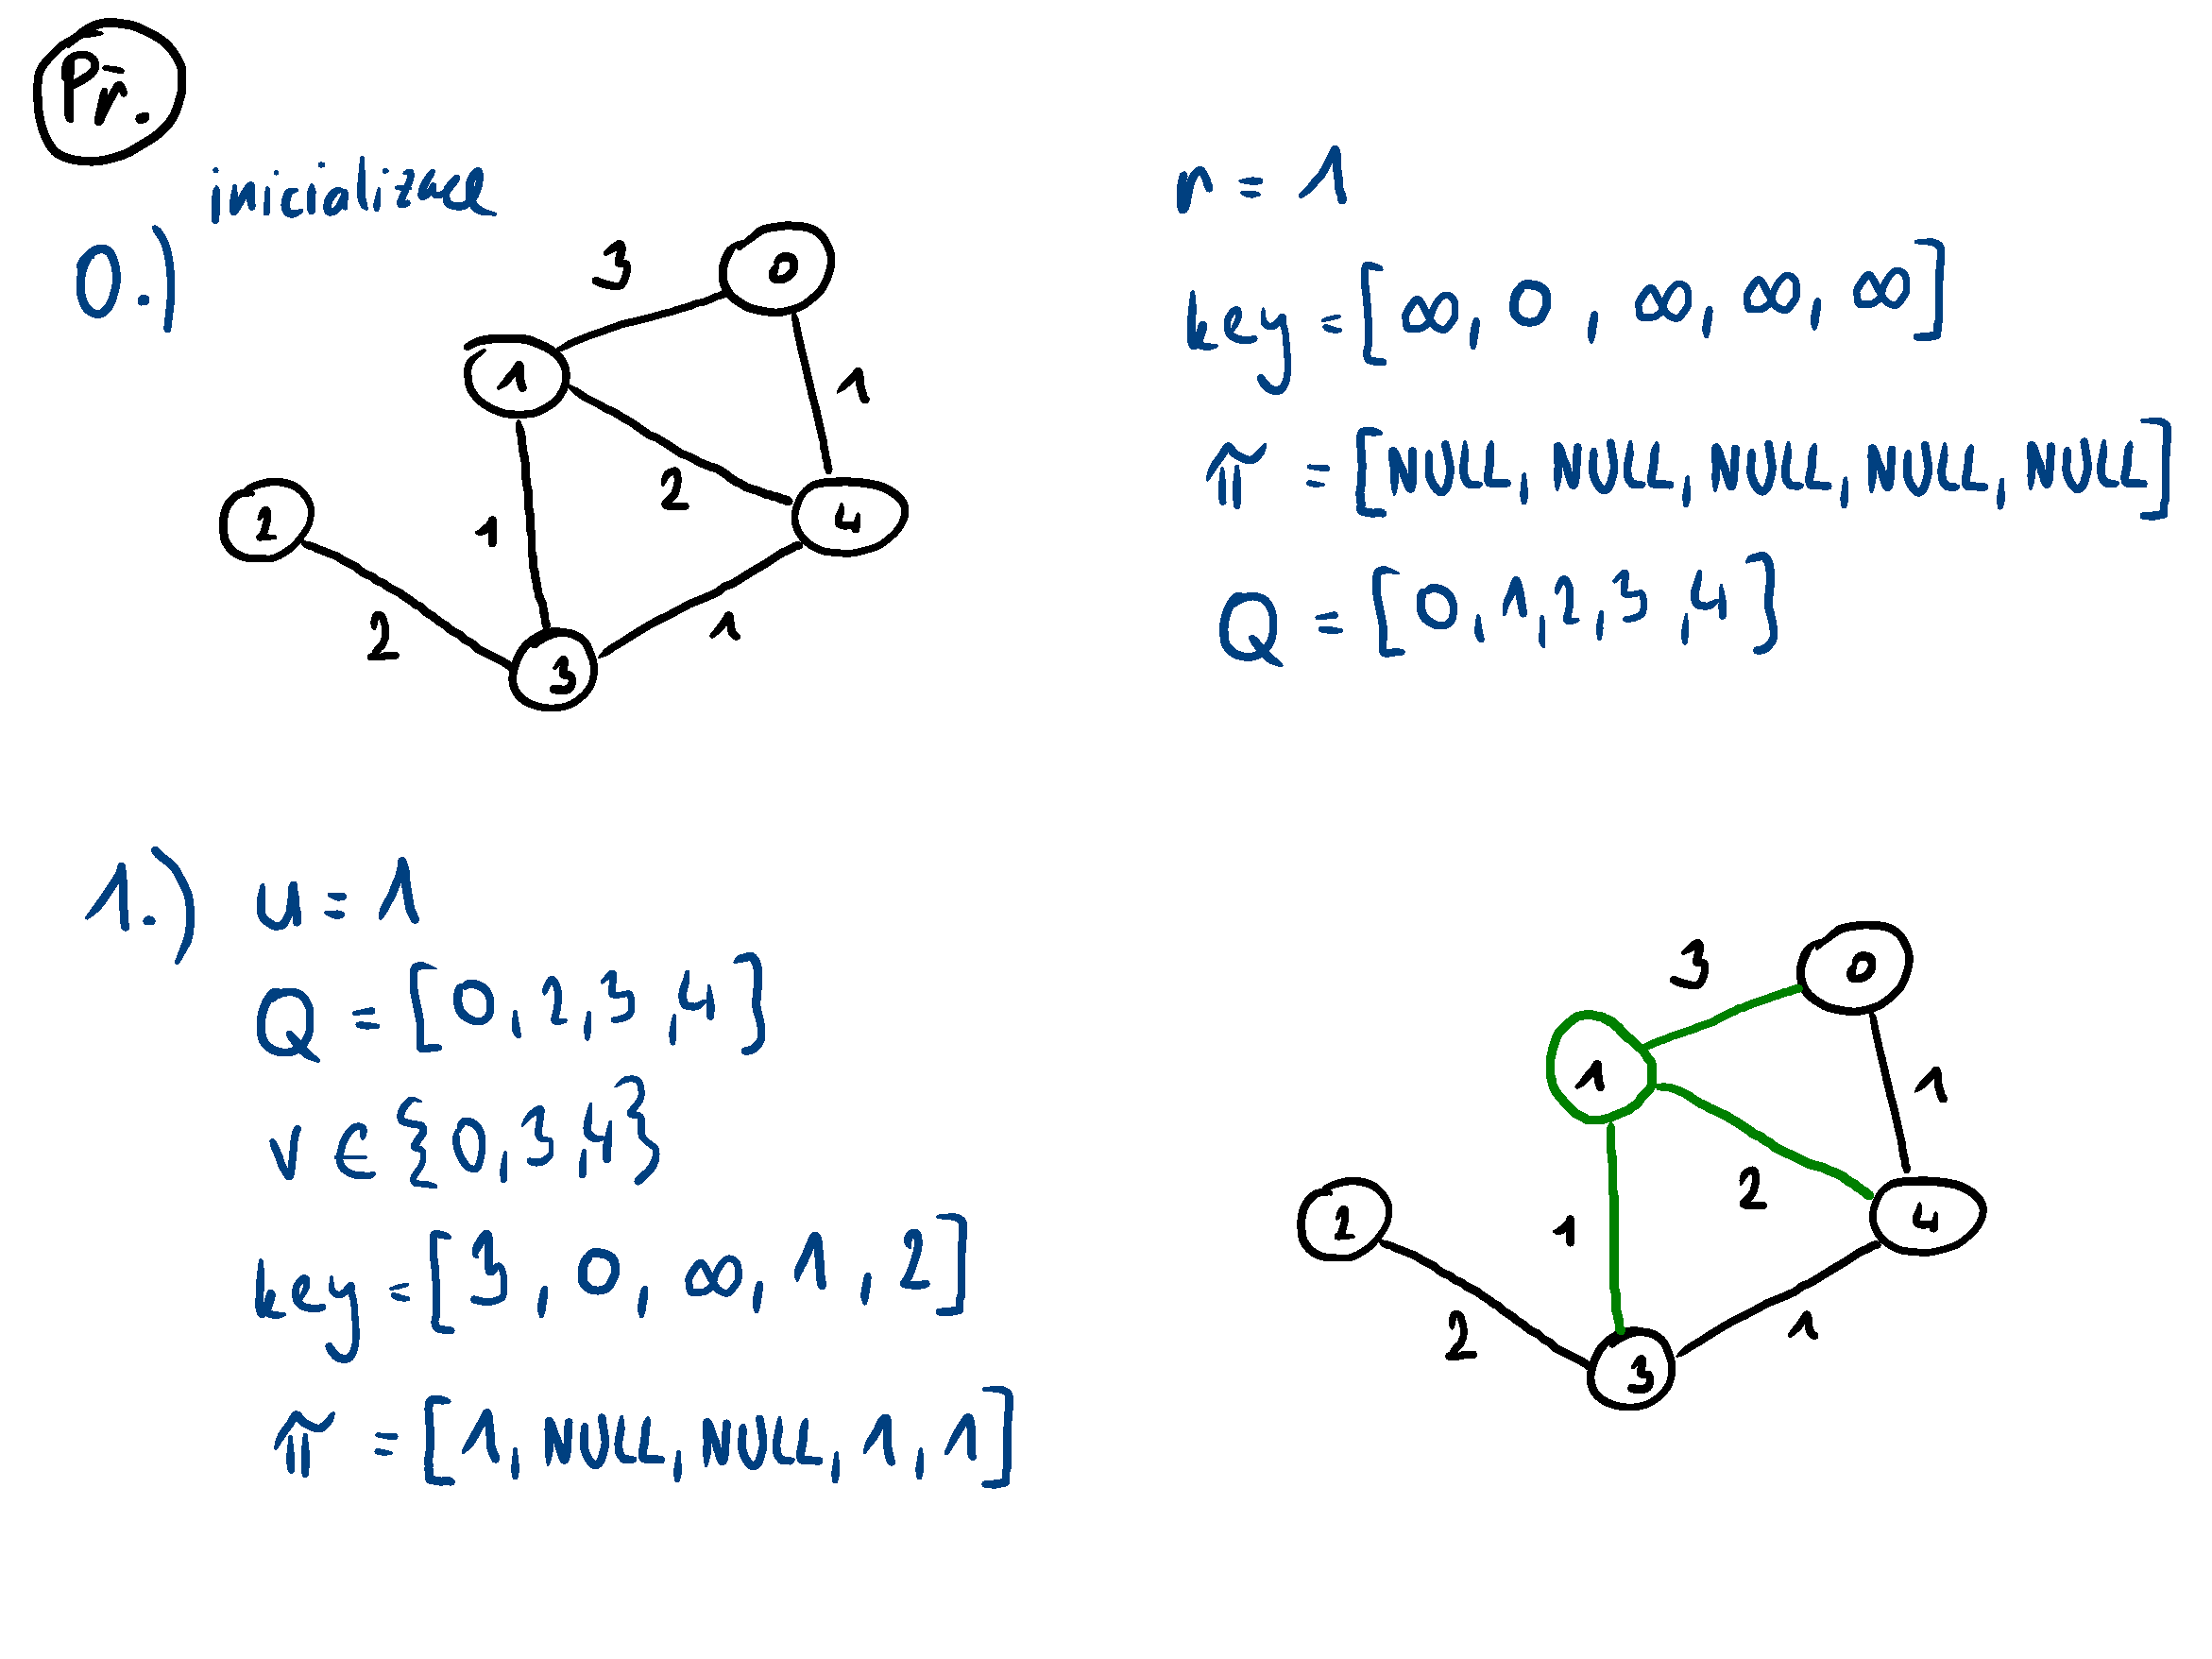
\includegraphics[width=0.9\linewidth]{gal_1/03-minimalni-kostry-16.pdf}
    \caption{Příklad, část 1.}
\end{figure}

\begin{figure}[H]
    \centering
    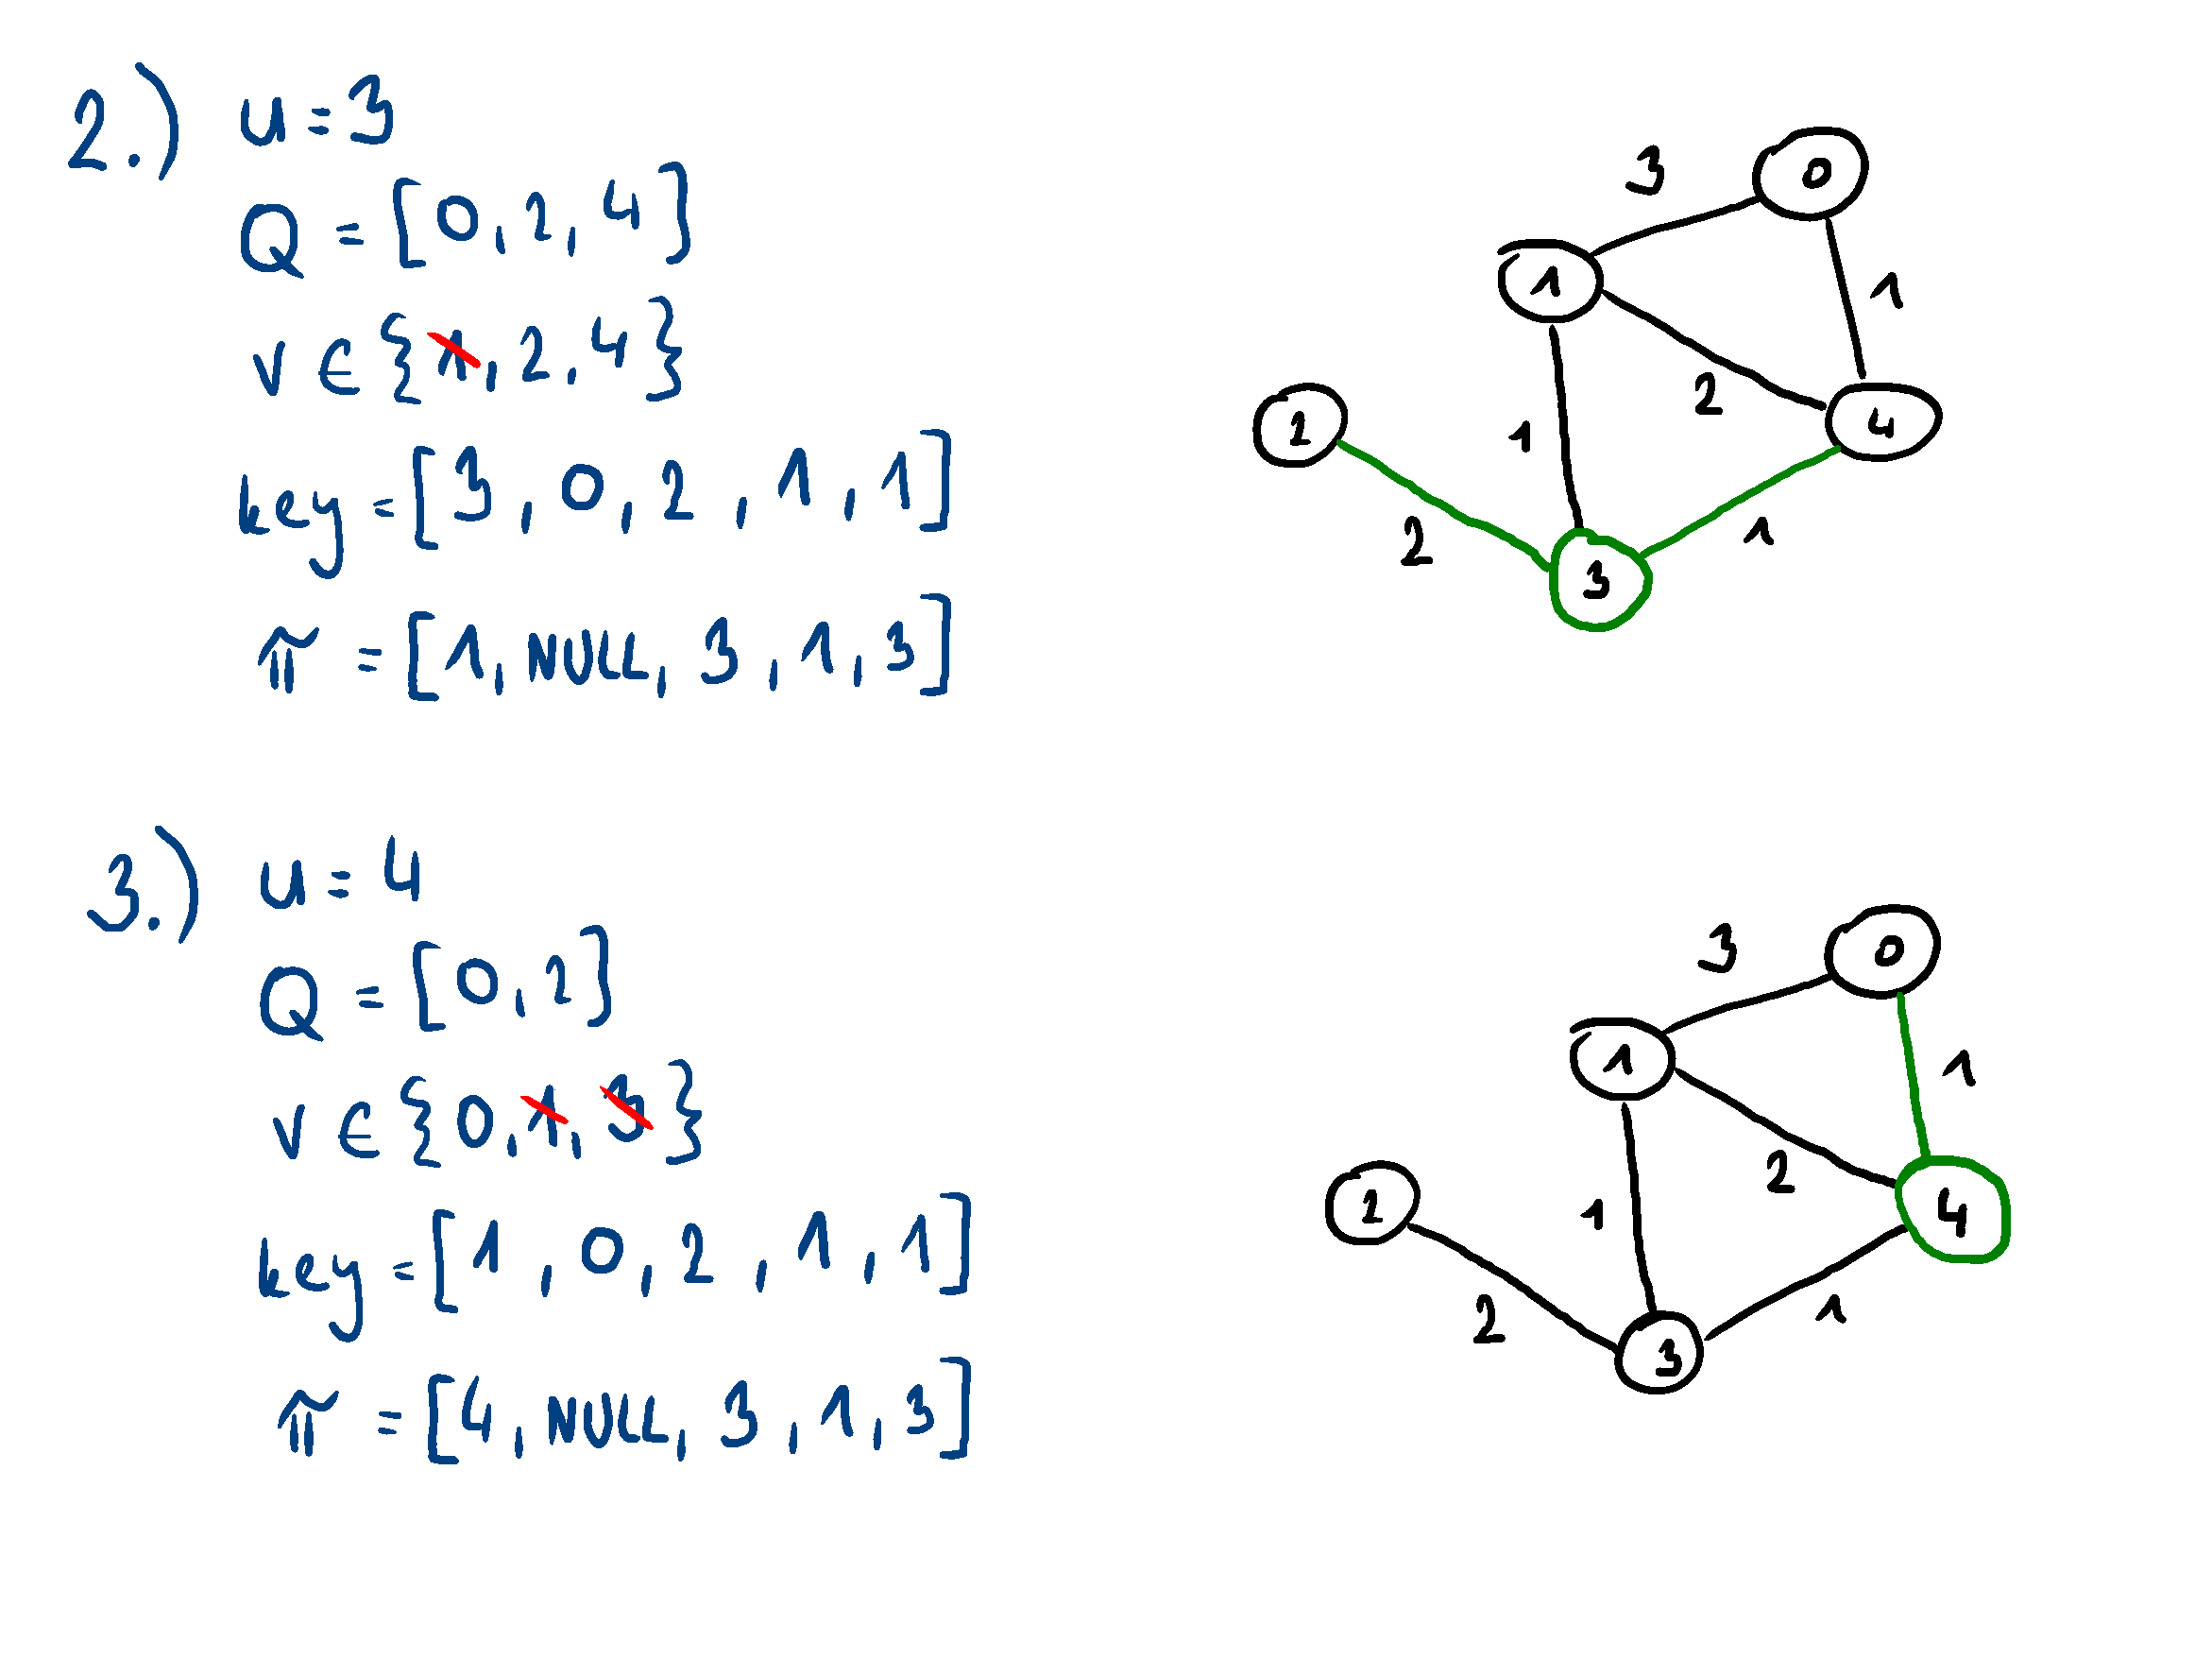
\includegraphics[width=0.9\linewidth]{gal_1/03-minimalni-kostry-17.pdf}
    \caption{Příklad, část 2.}
\end{figure}

\begin{figure}[H]
    \centering
    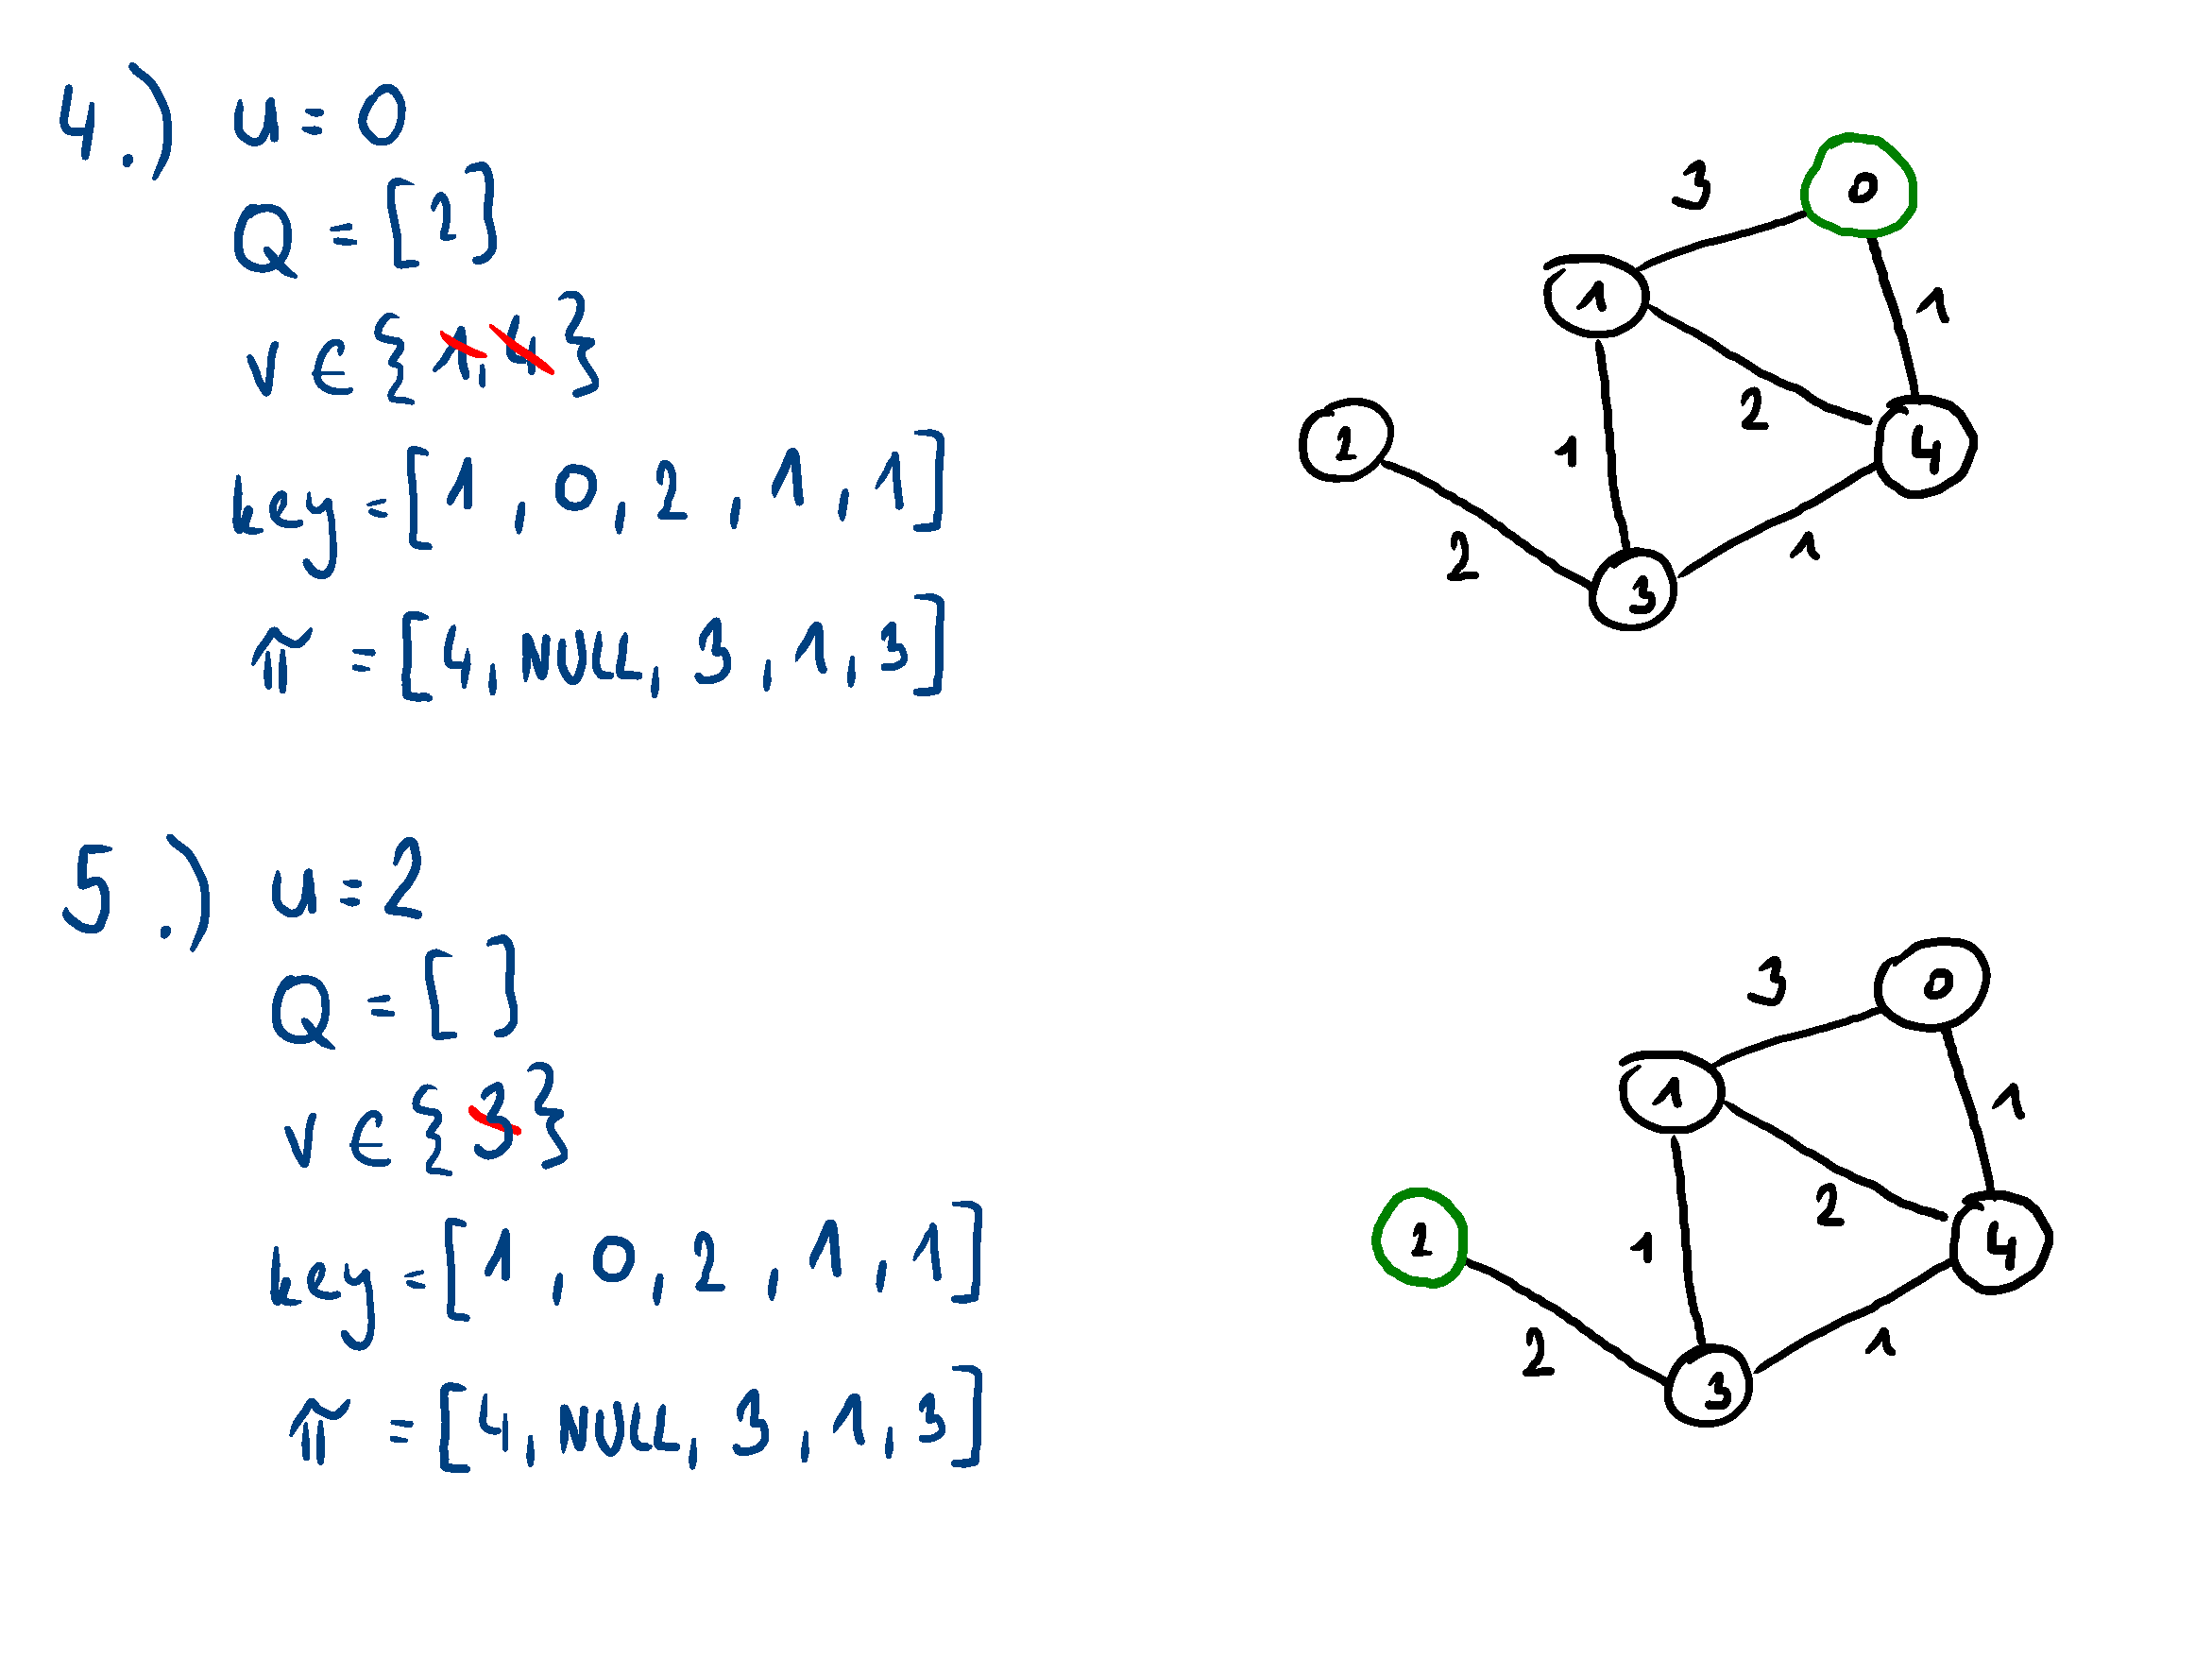
\includegraphics[width=0.9\linewidth]{gal_1/03-minimalni-kostry-18.pdf}
    \caption{Příklad, část 3.}
\end{figure}

\begin{figure}[H]
    \centering
    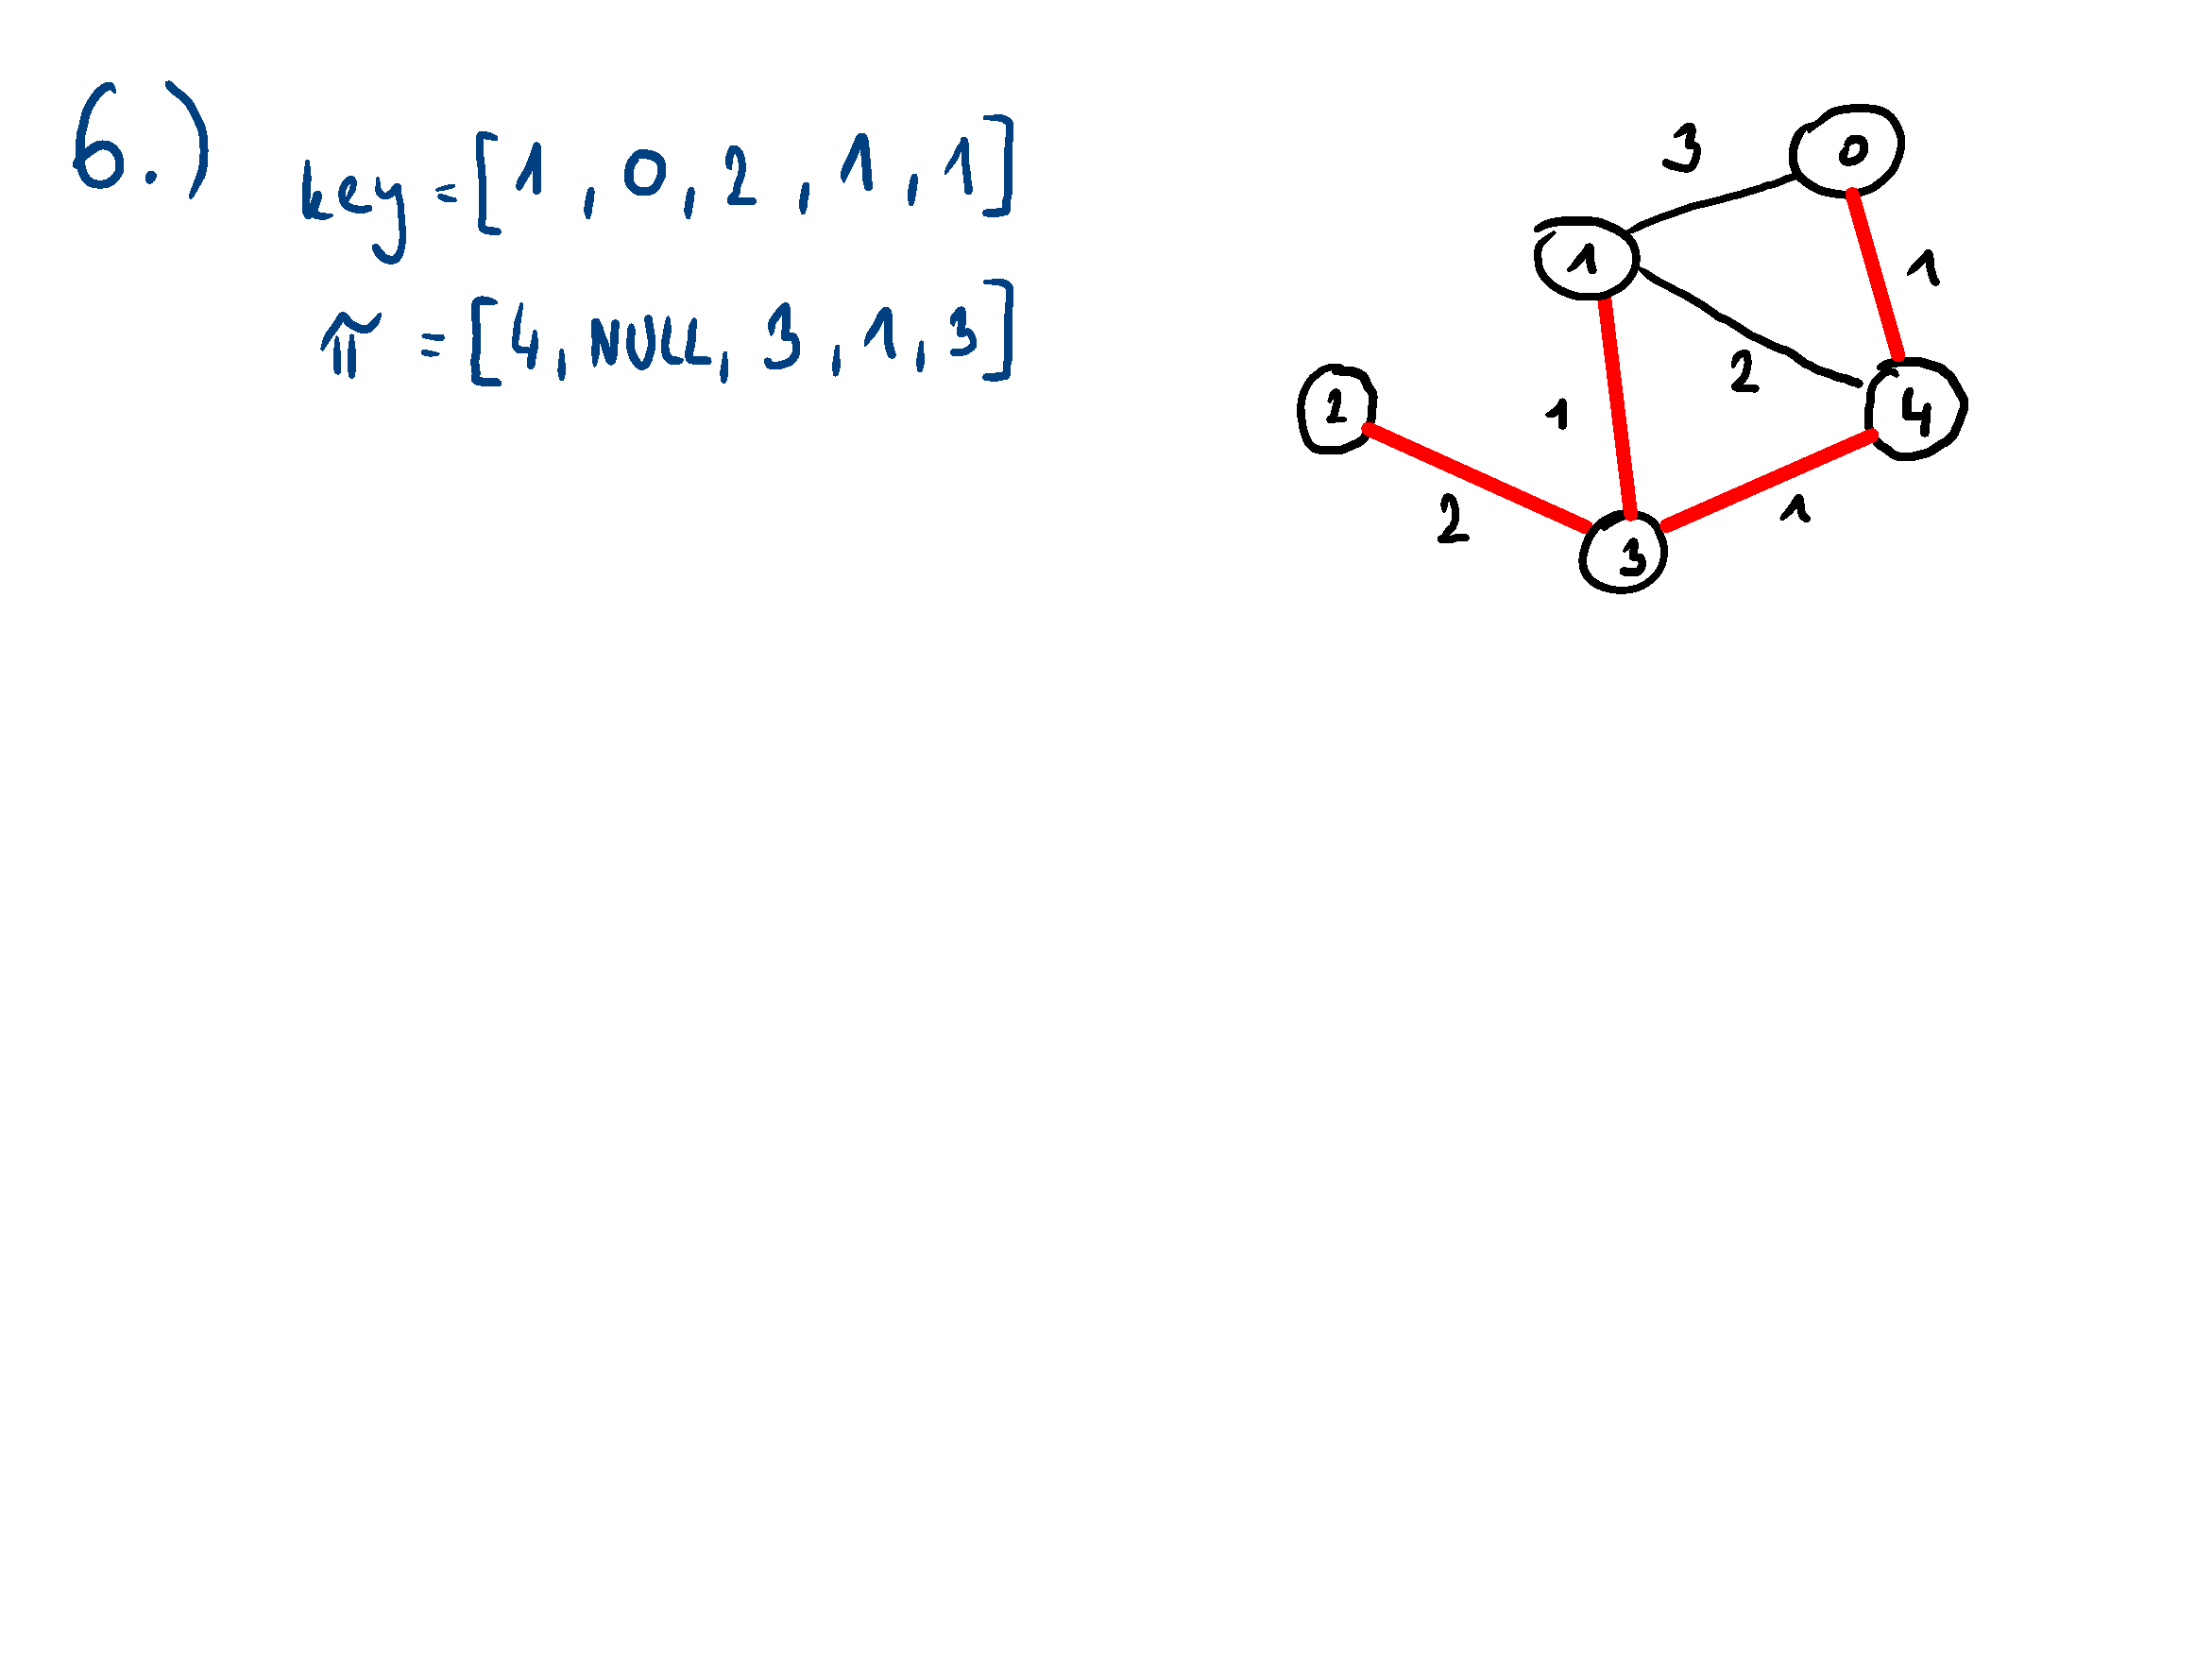
\includegraphics[width=0.9\linewidth]{gal_1/03-minimalni-kostry-19.pdf}
    \caption{Příklad, část 4.}
\end{figure}

\newpage

% VUT FIT MITAI
% MSZ 2021/2022
% Author: Vladimir Dusek
% Login: xdusek27

%%%%%%%%%%%%%%%%%%%%%%%%%%%%%%%%%%%%%%%%%%%%%%%%%%%%%%%%%%%%%%%%%%%%%%%%%%%%%%%%

\chapter{Hledání nejkratších cest ze zdrojového uzlu do všech ostatních uzlů grafu (Bellman-Fordův algoritmus, Dijkstrův algoritmus).}

%%%%%%%%%%%%%%%%%%%%%%%%%%%%%%%%%%%%%%%%%%%%%%%%%%%%%%%%%%%%%%%%%%%%%%%%%%%%%%%%

\section{Metadata}

\begin{compactitem}
    \item Předmět: Grafové algoritmy (GAL)
    \item Přednáška:
    \begin{compactitem}
        \item 7) Nejkratší cesty z jednoho vrcholu, Bellman-Fordův algoritmus, nejkratší cesta z jednoho vrcholu v orientovaných acyklických grafech.
        \item 8) Dijkstrův algoritmus. Nejkratší cesty ze všech vrcholů.
    \end{compactitem}
    \item Záznam:
    \begin{compactitem}
        \item 2020-11-05
    \end{compactitem}
\end{compactitem}

%%%%%%%%%%%%%%%%%%%%%%%%%%%%%%%%%%%%%%%%%%%%%%%%%%%%%%%%%%%%%%%%%%%%%%%%%%%%%%%%

\section{Úvod a kontext}

\textit{Viz. \uv{Úvod a kontext} v předchozích otázkách z tohoto předmětu.}

\paragraph*{Cena cesty} Nechť $G = (V, E)$ je ohodnocený graf s váhovou funkcí $w: E \mapsto \mathbb{R}$. Cena cesty $p = \langle v_o, v_1, \dots, v_k \rangle$ je suma $$
w(p) = \sum_{i=0}^k w(v_i, v_{i+1})
$$.

\paragraph*{Cena nejkratší cesty} Cena nejkratší cesty z $u$ do $v$ je $$
\delta(u, v) = \begin{cases}
    min( \{ w(p) : u \xRightarrow{\text{p}} v \} ) \\
    \infty ~ \text{pokud cesta neexistuje}
\end{cases}
$$.

\paragraph*{Nejkratší cesta} Nejkratší cesta z $u$ do $v$ je pak libovolná cesta $p$ taková, že $w(p) = \delta(u, v)$.

\paragraph*{Cena cesty se záporným cyklem} Pokud na cestě z $u$ do $v$ existuje záporný cyklus (cyklus jehož celková cena je záporná), pak $\delta(u, v) = - \infty$.

\paragraph*{Záporné ohodnocení hran} Pokud na cestě z $u$ do $v$ neexistuje záporný cyklus, tak algoritmy pracují dobře i se záporným ohodnocením hran.

\paragraph*{Reprezentace cesty} Cestu reprezentujeme pomocí pole předchůdců $\pi$.

\paragraph*{Hledání nejkratších cest ze všech uzlů do jednoho} Tento problém lze řešit stejnými algoritmy. Graf se transponuje (převrácení orientace hran), provede se algoritmus pro problém \uv{hledání nejkratších cest ze jednoho uzlu do všech ostatních uzlů} a poté se transponuje zpět.

\paragraph*{Reprezentace nejkratší cesty} Nejkratší cestu grafu $G = (V, E)$ reprezentujeme pomocí pole předchůdců $\pi$, kde $\pi[v]$ označuje předchůdce uzlu $v \in V$ na nejkratší cestě. Podgraf předchůdců pak je $G_{\pi} = (V_{\pi}, E_{\pi})$, $V_{\pi} = \{ v \in V : \pi[v] \neq \text{NULL} \} \cup \{ s \}$, $E_{\pi} = \{ (\pi[v], v) \in E : v \in V_{\pi} - \{ s \}$. V okamžiku dokončení algoritmu výpočtu nejkratších cest je $G_{\pi}$ strom nejkratších cest. Tj. kořenový strom obsahující nejkratší cesty ze zdroje $s$ do všech ostatních uzlů.

%%%%%%%%%%%%%%%%%%%%%%%%%%%%%%%%%%%%%%%%%%%%%%%%%%%%%%%%%%%%%%%%%%%%%%%%%%%%%%%%

\section{Pomocné funkce}

Představené algoritmy pracují z důvodu efektivity se sledy a nikoliv s cestami (bylo by nutné stále kontrolovat, zda nebyla porušena podmínka cesty), ačkoliv je problém nazývá hledání nejkratší cesty.

\bigskip\noindent\begin{minipage}{\linewidth}
\begin{lstlisting}[language=Python, caption={Pomocná inicializační funkce. Složitost je $\Theta(n)$, kde $n$ je počet uzlů.}]
def initialize_single_source(G, s):
    # G je graf
    # s je vychozi uzel
    for v in G.V:
        d[v] = INF  # d je pole vzdalenosti
        pi[v] = NULL  # pi je pole predchudcu
    d[s] = 0
\end{lstlisting}
\end{minipage}

\noindent\begin{minipage}{\linewidth}
\begin{lstlisting}[language=Python, caption={Pomocná funkce \textit{relax}. Složitost je $O(1)$.}]
def relax(u, v, w):
    # u a v jsou uzly grafu
    # w je vahova funkce
    if d[v] > d[u] + w(u, v):
        d[v] = d[u] + w(u, v)
        pi[v] = u
\end{lstlisting}
\end{minipage}

\begin{figure}[H]
    \centering
    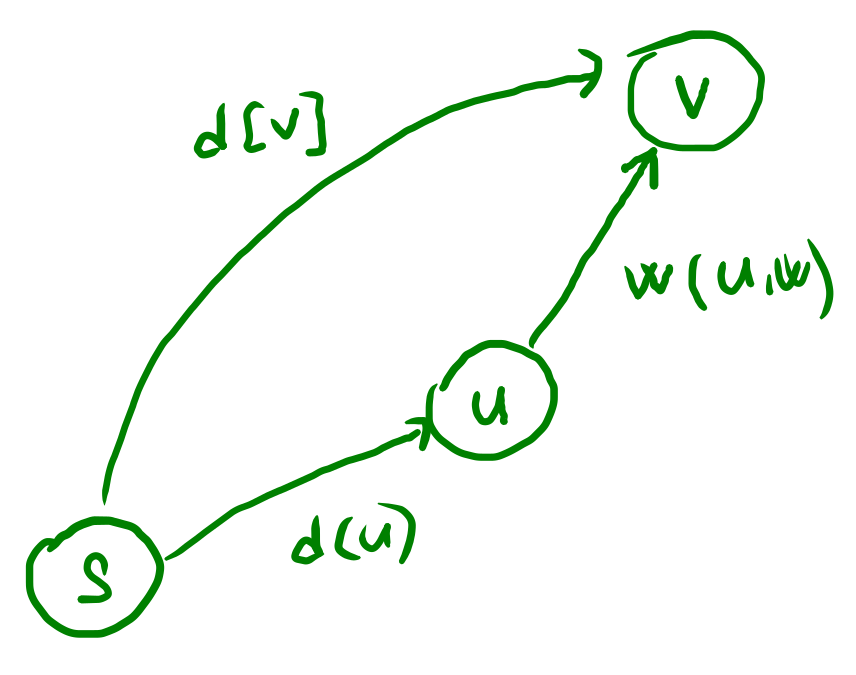
\includegraphics[width=0.4\linewidth]{gal_2/relax.png}
    \caption{Ukázka činnosti funkce \textit{relax}.}
\end{figure}

%%%%%%%%%%%%%%%%%%%%%%%%%%%%%%%%%%%%%%%%%%%%%%%%%%%%%%%%%%%%%%%%%%%%%%%%%%%%%%%%

\section{Bellman-Fordův algoritmus}

Slouží pro řešení v obecných grafech, mohou obsahovat cykly a záporné hrany. Záporné cykly je však nutné detekovat a vrátit specifickou hodnotu. V podstatě se jedná o \textit{brute force} algoritmus, provede se relaxace $n-1$-krát pro každou hranu.

\bigskip\noindent\begin{minipage}{\linewidth}
\begin{lstlisting}[language=Python, caption={Algoritmus Bellman-Ford. Proč $n-1$ iterací? Protože mezi libovolnými dvěma uzly v grafu, existuje cesta o maximálním počtu hran $n-1$.}]
def bellman_ford(G, s, w):
    # G je graf
    # s je vychozi uzel
    # w je vahova funkce

    # faze inicializace
    initialize_single_source(G, s)
    n = len(G.V) # pocet uzlu

    # faze relaxace: provedeni (n-1) * m relaxaci (m je pocet hran)
    for _ in range(0, n-1):
        for u, v in G.E:
            relax(u, v, w)

    # faze detekce zaporneho cyklu
    for u, v in G.E:
        if d[u] > d[v] + w(u, v):
            return NULL

    return pi
\end{lstlisting}
\end{minipage}

\subsection*{Složitost}

\begin{compactitem}
    \item Řádek 7, 8 -- $\Theta(1)$.
    \item Řádky 11, 12, 13 -- $(n-1) \cdot \Theta(m) = \Theta(n \cdot m)$, kde $n$ je počet uzlů a $m$ je počet hran grafu.
    \item Řádek 16, 17, 18 -- $\Theta(m)$.
    \item Celkem $\Theta(n \cdot m)$.
\end{compactitem}

\subsection*{Příklad}

\begin{figure}[H]
    \centering
    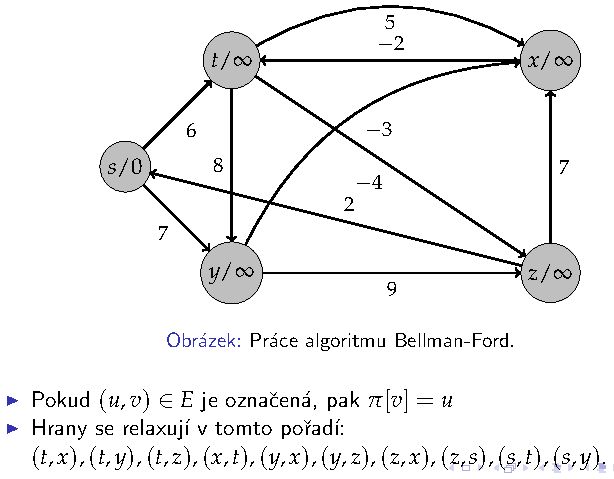
\includegraphics[width=0.75\linewidth]{gal_2/example_bellman_ford_p1.pdf}
    \caption{Příklad, část 1.}
\end{figure}

\begin{figure}[H]
    \centering
    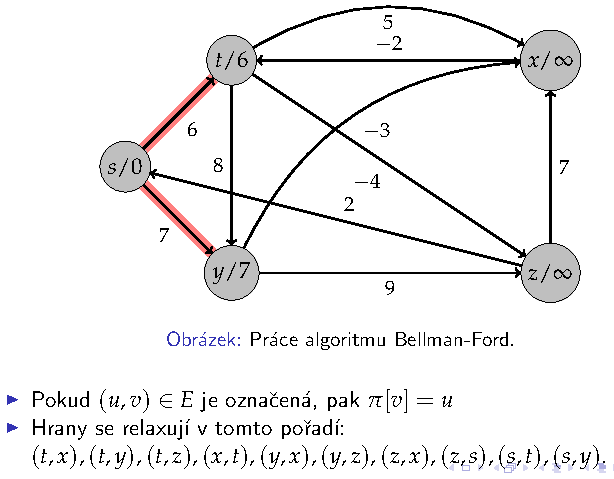
\includegraphics[width=0.75\linewidth]{gal_2/example_bellman_ford_p2.pdf}
    \caption{Příklad, část 2.}
\end{figure}

\begin{figure}[H]
    \centering
    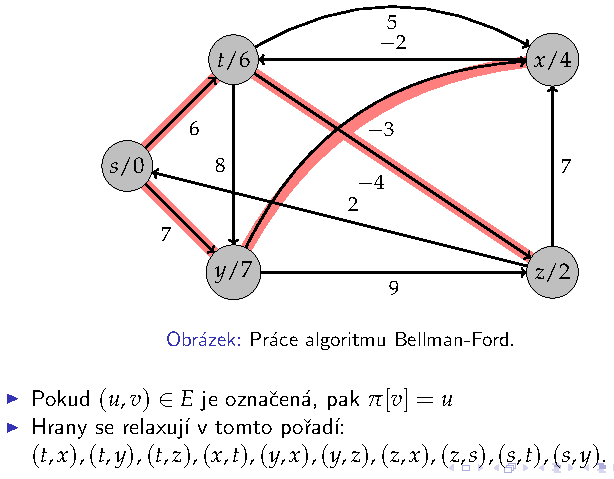
\includegraphics[width=0.75\linewidth]{gal_2/example_bellman_ford_p3.pdf}
    \caption{Příklad, část 3.}
\end{figure}

\begin{figure}[H]
    \centering
    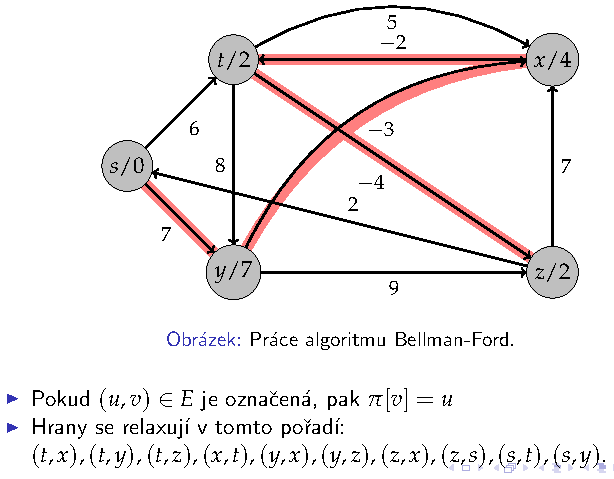
\includegraphics[width=0.75\linewidth]{gal_2/example_bellman_ford_p4.pdf}
    \caption{Příklad, část 4.}
\end{figure}

\begin{figure}[H]
    \centering
    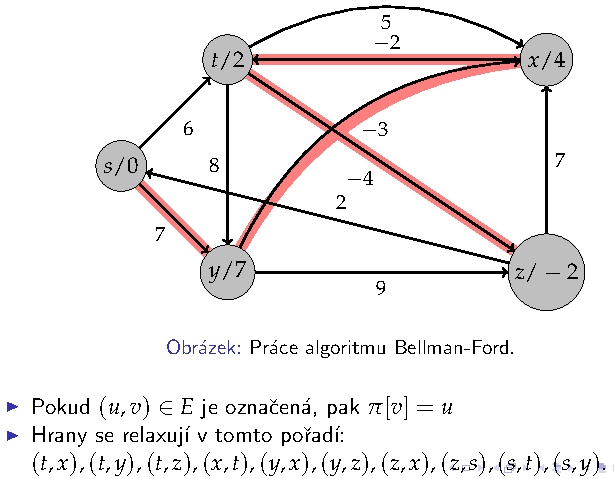
\includegraphics[width=0.75\linewidth]{gal_2/example_bellman_ford_p5.pdf}
    \caption{Příklad, část 5.}
\end{figure}

%%%%%%%%%%%%%%%%%%%%%%%%%%%%%%%%%%%%%%%%%%%%%%%%%%%%%%%%%%%%%%%%%%%%%%%%%%%%%%%%

\section{Dijkstrův algoritmus}

Slouží pro řešení v acyklických grafech bez záporných hran. Pro takto omezený problém existují rychlejší algoritmy než pro problém v obecných grafech.

\bigskip\noindent\begin{minipage}{\linewidth}
\begin{lstlisting}[language=Python, caption={Algoritmus Dijkstra.}]
def dijkstra(G, s, w):
    # G je graf
    # s je vychozi uzel
    # w je vahova funkce

    # faze inicializace
    initialize_single_source(G, s)
    Q = Queue(G.V) # prioritni fronta uzlu
    S = {} # mnozina uzlu, ktera uz byla prozkoumana

    # faze relaxace
    while not Q.empty():
        u = Q.extract_min(d) # vrati prvek z Q s nejmensi hodnotou v d
        S += {u}
        # pro vsechny sousedy uzlu u (Adj je seznam sousedu)
        for v in Adj[u]:
            relax(u, v, w)

        Q.decrease_key(d) # aktualizace prioritni fronty

    return d, pi
\end{lstlisting}
\end{minipage}

\subsection*{Složitost}

\begin{compactitem}
    \item Předpokládejme implementaci prioritní fronty pomocí pole.
    \item Řádek 8, 18 -- $O(1)$.
    \item Řádek 11 -- While cyklus se provede $n$-krát, kde $n$ je počet uzlů.
    \item Řádek 12 -- $O(n)$, najítí minima v poli uzlů. Celkově (s cyklem) $O(n^2)$.
    \item Řádek 16 -- $O(m)$, pro všechny hrany. Celkově (s cyklem) $O(m \cdot n)$.
    \item Celkem $O(n^2 + m) = O(n^2)$.
    \item Pro řídké grafy lze využít implementaci fronty pomocí binární haldy a získat tak $O(m \cdot \log(n))$.
    \item Při implementaci fronty pomocí Fibonacciho haldy dostaneme časovou složitost $O(n \cdot \log(n) + m)$.
\end{compactitem}

\subsection*{Příklad}

\begin{figure}[H]
    \centering
    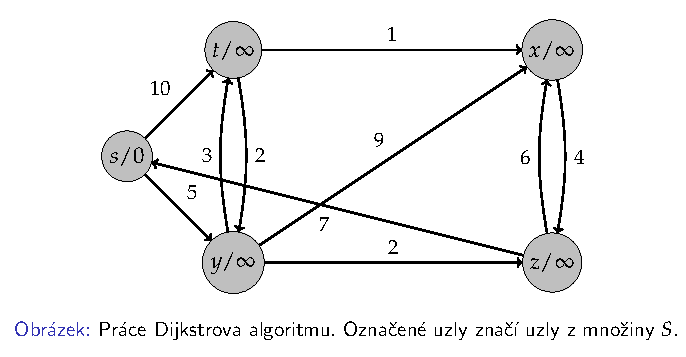
\includegraphics[width=0.80\linewidth]{gal_2/example_dijkstra_p1.pdf}
    \caption{Příklad, část 1.}
\end{figure}

\begin{figure}[H]
    \centering
    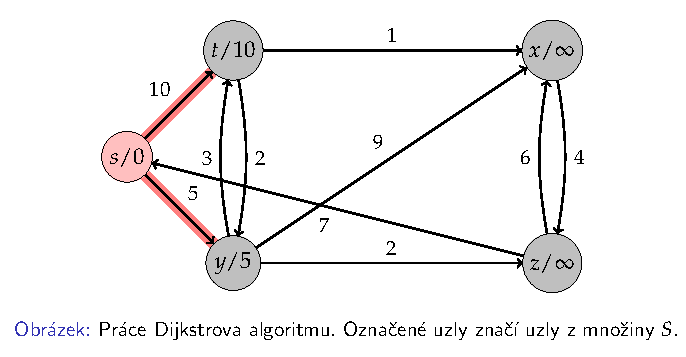
\includegraphics[width=0.80\linewidth]{gal_2/example_dijkstra_p2.pdf}
    \caption{Příklad, část 2.}
\end{figure}

\begin{figure}[H]
    \centering
    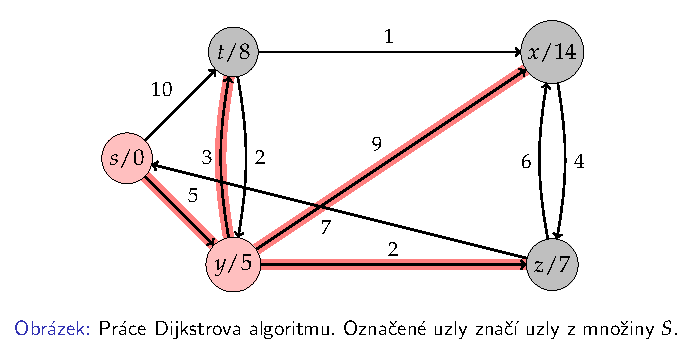
\includegraphics[width=0.80\linewidth]{gal_2/example_dijkstra_p3.pdf}
    \caption{Příklad, část 3.}
\end{figure}

\begin{figure}[H]
    \centering
    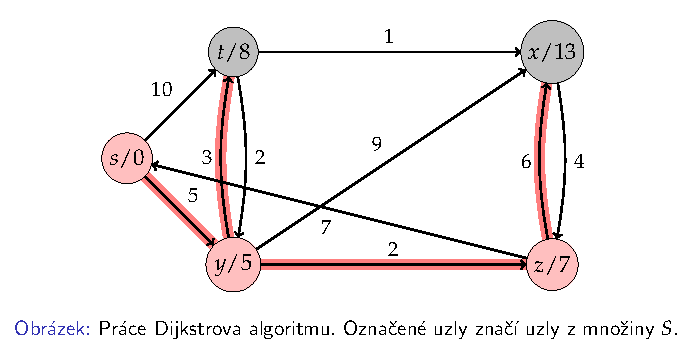
\includegraphics[width=0.80\linewidth]{gal_2/example_dijkstra_p4.pdf}
    \caption{Příklad, část 4.}
\end{figure}

\begin{figure}[H]
    \centering
    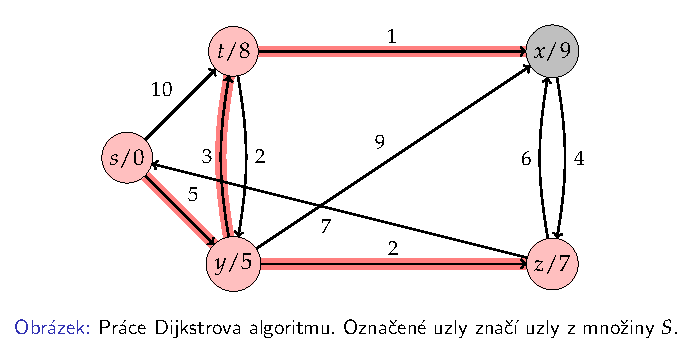
\includegraphics[width=0.80\linewidth]{gal_2/example_dijkstra_p5.pdf}
    \caption{Příklad, část 5.}
\end{figure}

\begin{figure}[H]
    \centering
    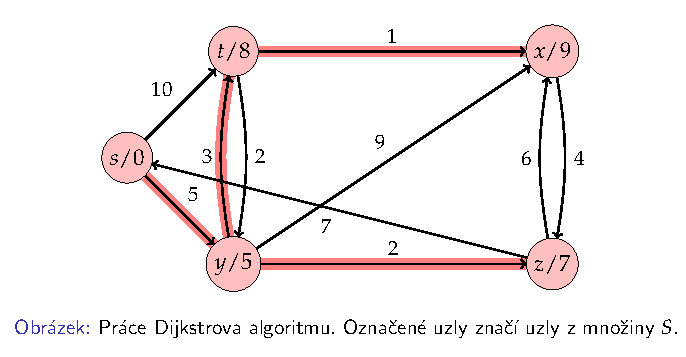
\includegraphics[width=0.80\linewidth]{gal_2/example_dijkstra_p6.pdf}
    \caption{Příklad, část 6.}
\end{figure}

\newpage

% VUT FIT MITAI
% MSZ 2021/2022
% Author: Vladimir Dusek
% Login: xdusek27

%%%%%%%%%%%%%%%%%%%%%%%%%%%%%%%%%%%%%%%%%%%%%%%%%%%%%%%%%%%%%%%%%%%%%%%%%%%%%%%%

\chapter{Klasifikace algoritmů volby koordinátora, algoritmus Bully a jeho složitost.}

%%%%%%%%%%%%%%%%%%%%%%%%%%%%%%%%%%%%%%%%%%%%%%%%%%%%%%%%%%%%%%%%%%%%%%%%%%%%%%%%

\section{Metadata}

\begin{itemize}
    \item Předmět: Prostředí distribuovaných aplikací (PDI)
    \item Přednáška:
    \begin{itemize}
        \item 7) Synchronizace
    \end{itemize}
    \item Záznam:
    \begin{itemize}
        \item 2020-11-02
    \end{itemize}
\end{itemize}

%%%%%%%%%%%%%%%%%%%%%%%%%%%%%%%%%%%%%%%%%%%%%%%%%%%%%%%%%%%%%%%%%%%%%%%%%%%%%%%%

\section{Úvod a kontext}

\begin{itemize}
    \item Mějme množinu procesů v rámci distribuovaného systému. Řešíme problém  nalezení shody na nějaké věci (synchronizační problém). Problém můžeme rozdělit na dvě situace:
    \begin{itemize}
        \item \textbf{Problém volby koordinátora} -- Výběr jednoho z procesů, který bude vedoucím procesem (koordinátor). Tento proces pak může vykonat určitou činnost nebo může sloužit ostatním procesům k realizaci  význačné role v systému.
        \item \textbf{Problém vzájemného vyloučení} -- Předpokládejme, že konkrétní zdroj může v daném okamžiku používat pouze jeden proces. Tento problém se běžně vyskytuje ve víceprocesorových systémech, ale také v distribuovaných systémech.
    \end{itemize}
    \item Synchronizační problémy lze v rámci operačních systémů nebo multiprocesorových systémů řešit pomocí provádění atomických operací, sdílené paměti apod. (je pro ně podpora v rámci operačního systému nebo hardwaru). V distribuovaných systémech nic takového není z principu možné a proto se synchronizační problémy řeší pomocí zasílání zprav, resp. algoritmicky.
\end{itemize}

%%%%%%%%%%%%%%%%%%%%%%%%%%%%%%%%%%%%%%%%%%%%%%%%%%%%%%%%%%%%%%%%%%%%%%%%%%%%%%%%

\section{Problém volby koordinátora}

\begin{itemize}
    \item Předpokládáme:
    \begin{itemize}
        \item Každý proces má unikátní ID.
        \item Procesy neznají stav (běžící, neběžící) dalších procesů.
        \item Každý proces zná ID dalších procesů (záleží na topologii).
    \end{itemize}
    \item Cíl:
    \begin{itemize}
        \item Dosáhnutí shody mezi všemi procesy na procesu, který je koordinátor.
        \item Kritérium výběru koordinátora může být různé. Např. na základě proces ID (proces s největším ID se stane koordinátorem).
    \end{itemize}
\end{itemize}

%%%%%%%%%%%%%%%%%%%%%%%%%%%%%%%%%%%%%%%%%%%%%%%%%%%%%%%%%%%%%%%%%%%%%%%%%%%%%%%%

\section{Bully algoritmus}

Pro topologii každý s každým -- každý proces může komunikovat s každým dalším procesem. Používá tři druhy zpráv: ELECTION, OK, COORDINATOR.

\subsection*{Postup}

\begin{itemize}
    \item Proces P, který má podezření, že chybí koordinátor, může zahájit volby.
    \begin{enumerate}
        \item Proces P odešle zprávu ELECTION všem procesům s větším ID.
        \item Pokud nikdo neodpoví, P vyhrává volby a stává se koordinátorem.
        \item Pokud některý z procesů s větším ID odpoví (zpráva OK), tak přebírá řízení a práce P je ukončena.
        \item Pokud P obdrží zprávu ELECTION od procesů s menším ID, pošle jim odpověď OK na zablokování procesů.
    \end{enumerate}
    \item Nakonec zůstane pouze P (nový koordinátor), který o tom informuje ostatní zasláním zprávy COORDINATOR.
    \item Pokud se proces probudí nebo je restartován, první akcí je vyvolání voleb.
\end{itemize}

\subsection*{Složitost}

Složitost z hlediska počtu zpráv.

\bigskip\noindent Nejhorší případ (iniciátor s nejmenším ID):

\begin{itemize}
    \item $(n-1)$ iterací
    \item $2(n-1)$ zpráv ELECTION a OK pro každou iteraci
    \item $(n-1)$ zpráv COORDINATOR
    \item Celkem: $(n-1) \times 2(n-1) + (n-1) \approx n^2$
\end{itemize}

\noindent Nejlepší případ (iniciátor s největším ID):

\begin{itemize}
    \item $(n-1)$ zpráv COORDINATOR
    \item Celkem: $(n-1)$
\end{itemize}

\subsection*{Příklad}

\begin{figure}[H]
    \centering
    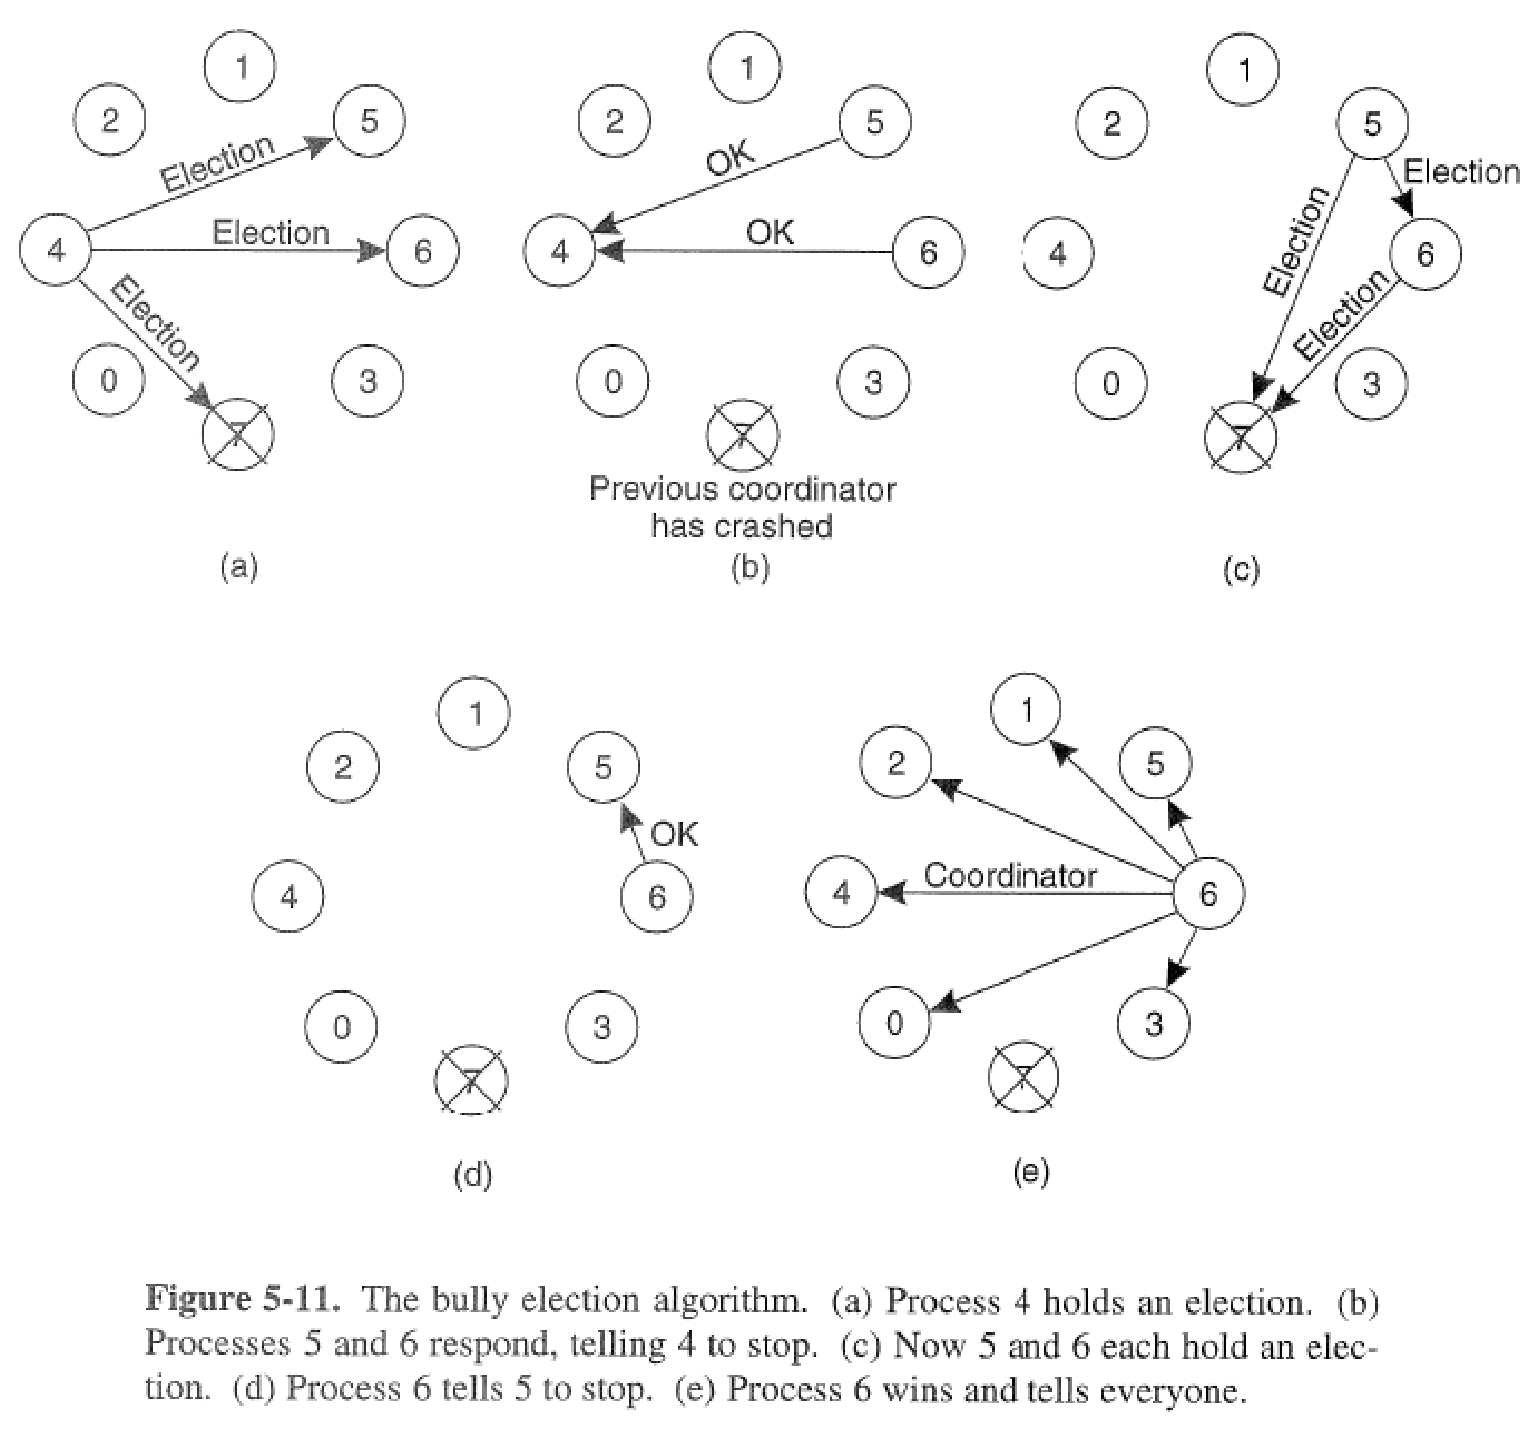
\includegraphics[width=1\linewidth]{pdi_1/example_bully.pdf}
    \caption{Příklad činnosti Bully algoritmu.}
\end{figure}

%%%%%%%%%%%%%%%%%%%%%%%%%%%%%%%%%%%%%%%%%%%%%%%%%%%%%%%%%%%%%%%%%%%%%%%%%%%%%%%%

\section{Ring Algoritmus}

Pro kruhovou topologii -- procesy jsou uspořádané do kruhu podle svého proces ID.
Každý proces musí vědět nejenom o svém následovníkovi, ale také o jeho následníkovi, který funguje jako \uv{záloha}, v případě že by se přímý následník stal nedostupný. Používá dva druhy zpráv: ELECTION, COORDINATOR.

\subsection*{Postup}

\begin{itemize}
    \item Proces P, který má podezření, že chybí koordinátor, může zahájit volby.
    \begin{enumerate}
        \item Zašle zprávu ELECTION obsahující jeho ID dalšímu procesu (pokud další proces nereaguje, proces P zašle stejnou zprávu dalšímu v kruhu).
        \item Každý člen topologie přijme zprávu ELECTION, přidá do ní své ID a přepošle zprávu dalšímu procesu.
    \end{enumerate}
    \item Když se zpráva vrátí k procesu P, je zpráva převedena na zprávu  COORDINATOR a poslána následujícímu procesu v topologii, aby bylo možné nahlásit:
    \begin{enumerate}
        \item Novým koordinátorem se stává proces s nejvyšším ID.
        \item Členové sítě jsou stále aktivní.
    \end{enumerate}
    \item Po síti může obíhat více zpráv zároveň.
\end{itemize}

\subsection*{Složitost}

Složitost z hlediska počtu zpráv.

\bigskip\noindent Vždy $2n \approx n$ zpráv. Jedno kolečko \uv{oběhne} zpráva ELECTION a druhé zpráva COORDINATOR.

\subsection*{Příklad}

\begin{figure}[H]
    \centering
    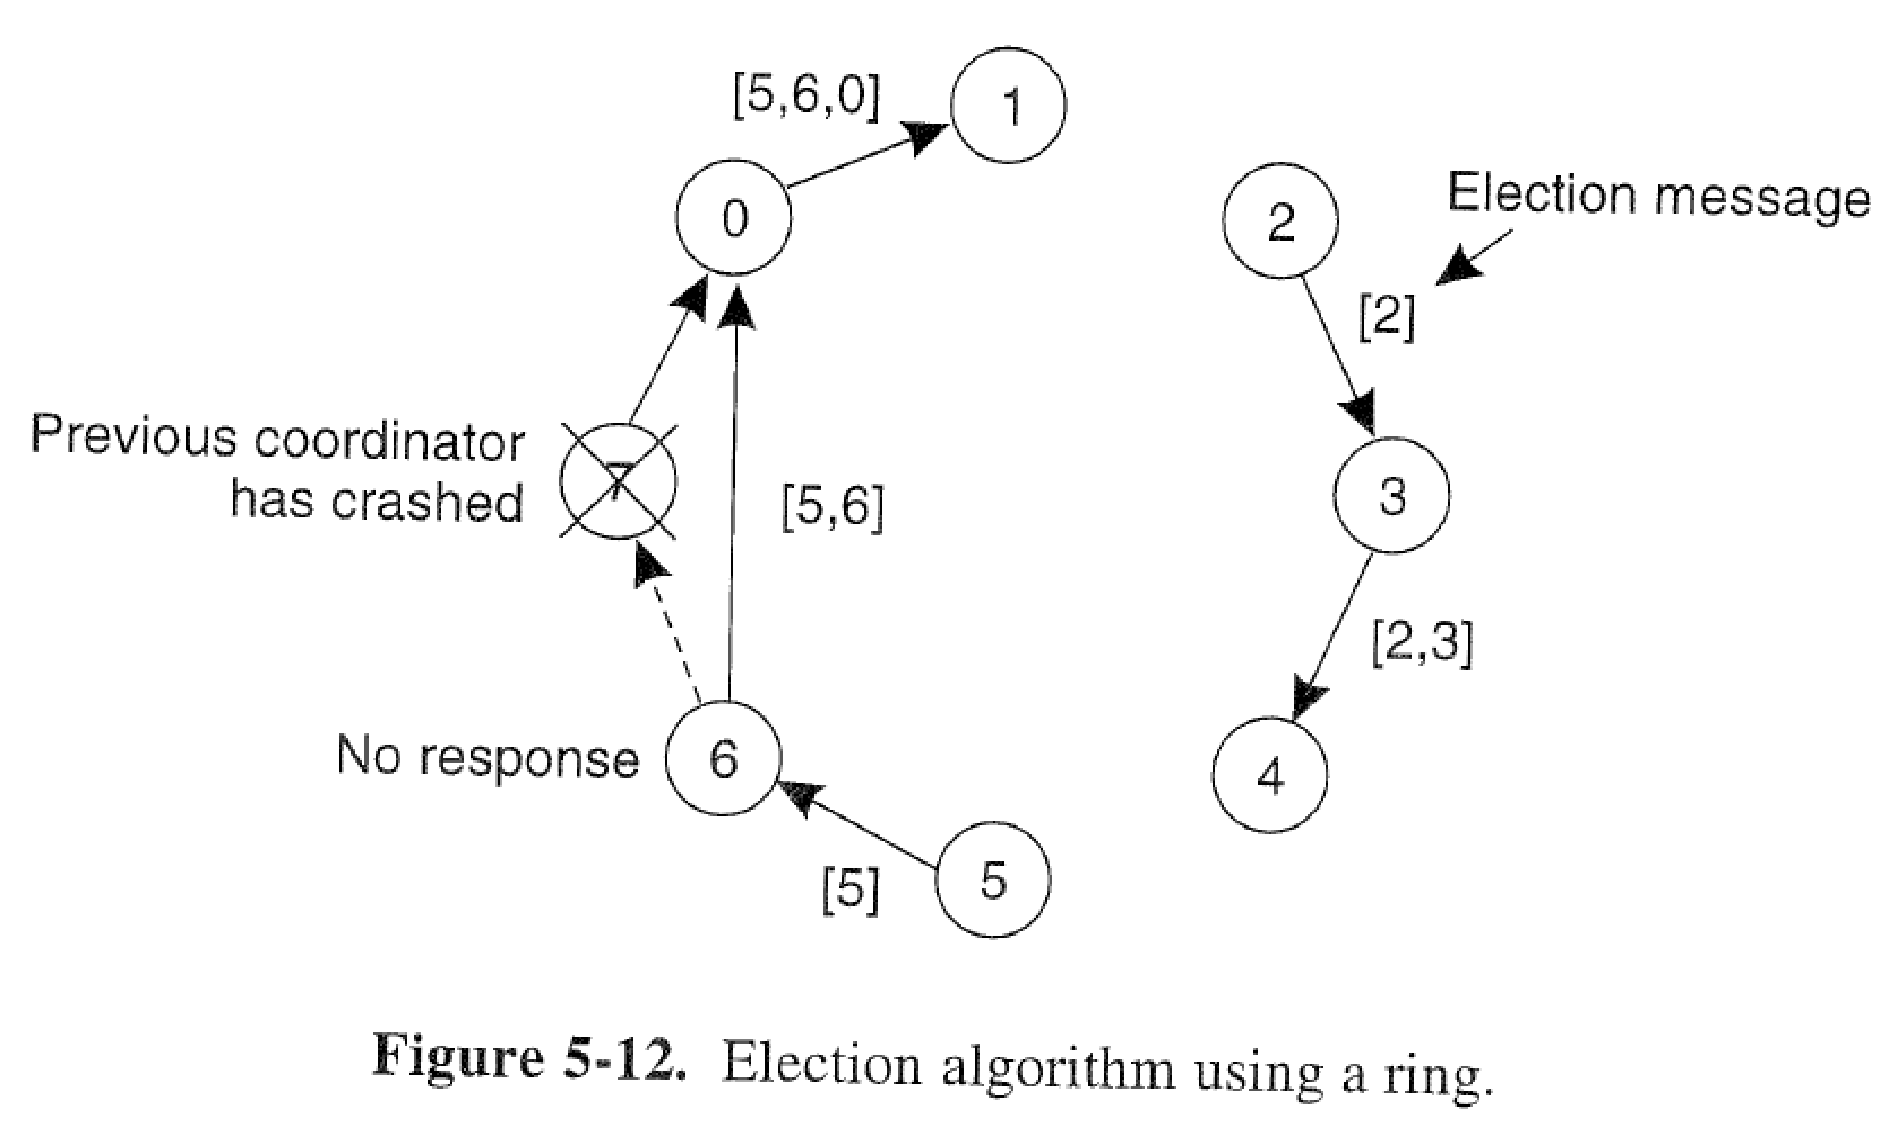
\includegraphics[width=1\linewidth]{pdi_1/example_ring.pdf}
    \caption{Příklad činnosti Ring algoritmu.}
\end{figure}

%%%%%%%%%%%%%%%%%%%%%%%%%%%%%%%%%%%%%%%%%%%%%%%%%%%%%%%%%%%%%%%%%%%%%%%%%%%%%%%%

\section{Algoritmus pro obecnou topologii}

Předpokládáme, že nemáme ani kruhovou topologii ani spojení každý s každým. Např.: peer-to-peer sítě, sensorové sítě, \dots

\subsection*{Postup}

\begin{itemize}
    \item V první iteraci se broadcastem posílá zpráva ELECTION.
    \item Každý uzel si uloží od kterého souseda dostal zprávu ELECTION jako první. Tím vzníká kostra grafu (\textit{spanning tree}).
    \item Uložený soused je poté využijí pro zpětnou komunikaci. To znamená, že další komunikace už probíhá přes strom, nikoliv přes broadcast. Tím je ušetřena některé komunikace.
\end{itemize}

\subsection*{Složitost}

Složitost z hlediska počtu zpráv.

\begin{itemize}
    \item Inicializační broadcast: počet hran grafu.
    \item Odpověď: počet hran kostry grafu.
    \item Result broadcast: počet hran kostry grafu.
\end{itemize}

\subsection*{Příklad}

\begin{figure}[H]
    \centering
    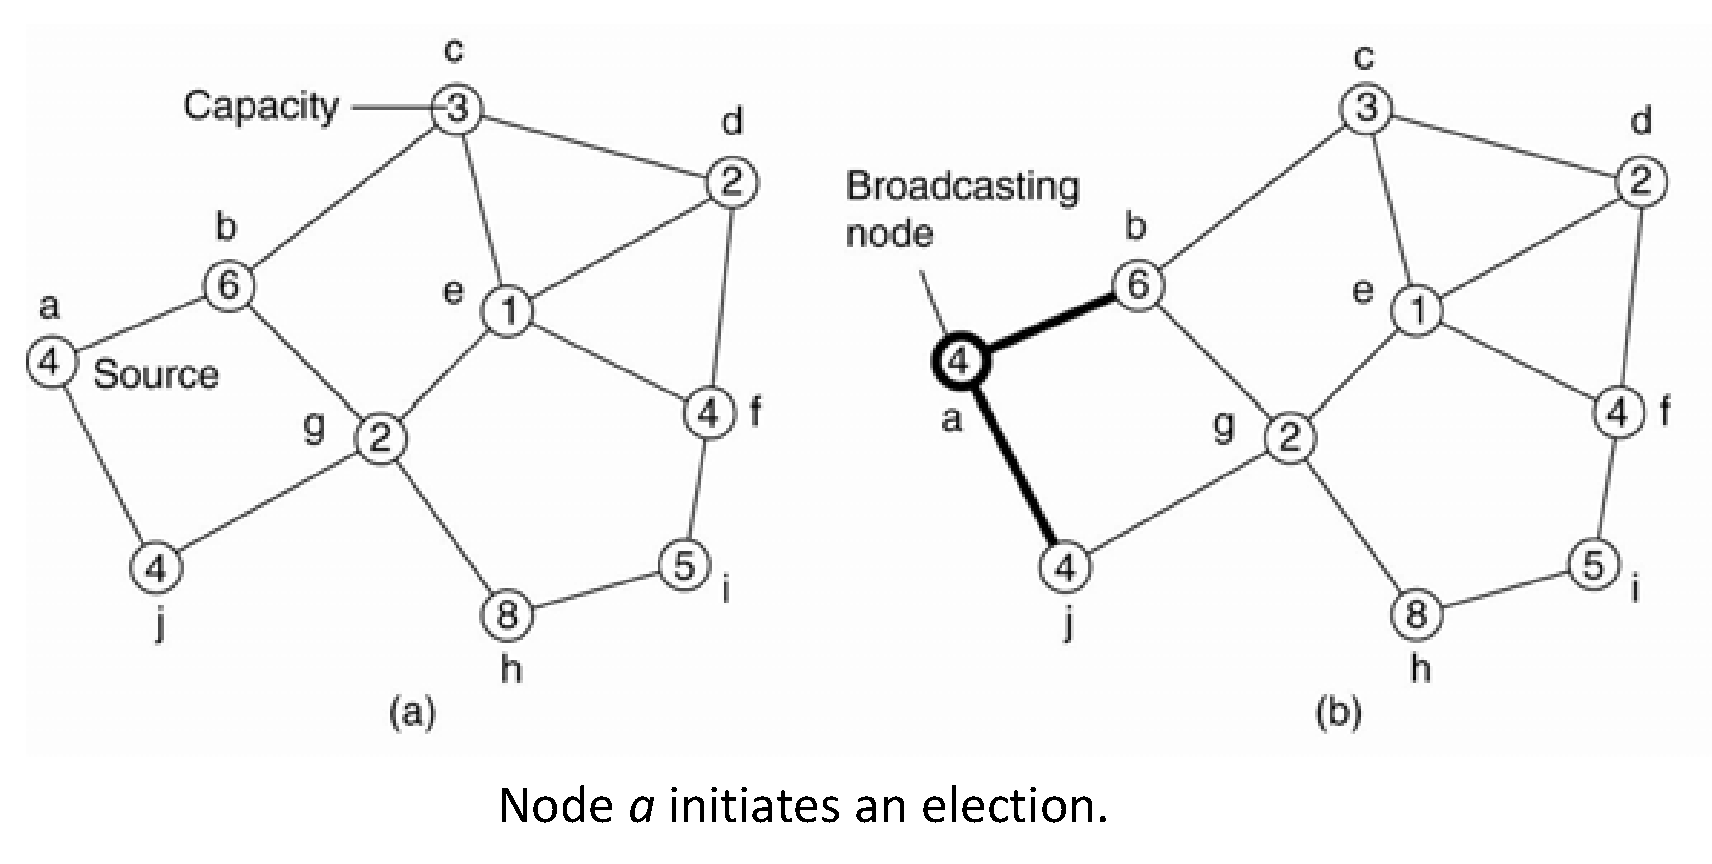
\includegraphics[width=1\linewidth]{pdi_1/example_general_topology_p1.pdf}
    \caption{Příklad činnosti algoritmu pro obecnou topologii, část 1.}
\end{figure}

\begin{figure}[H]
    \centering
    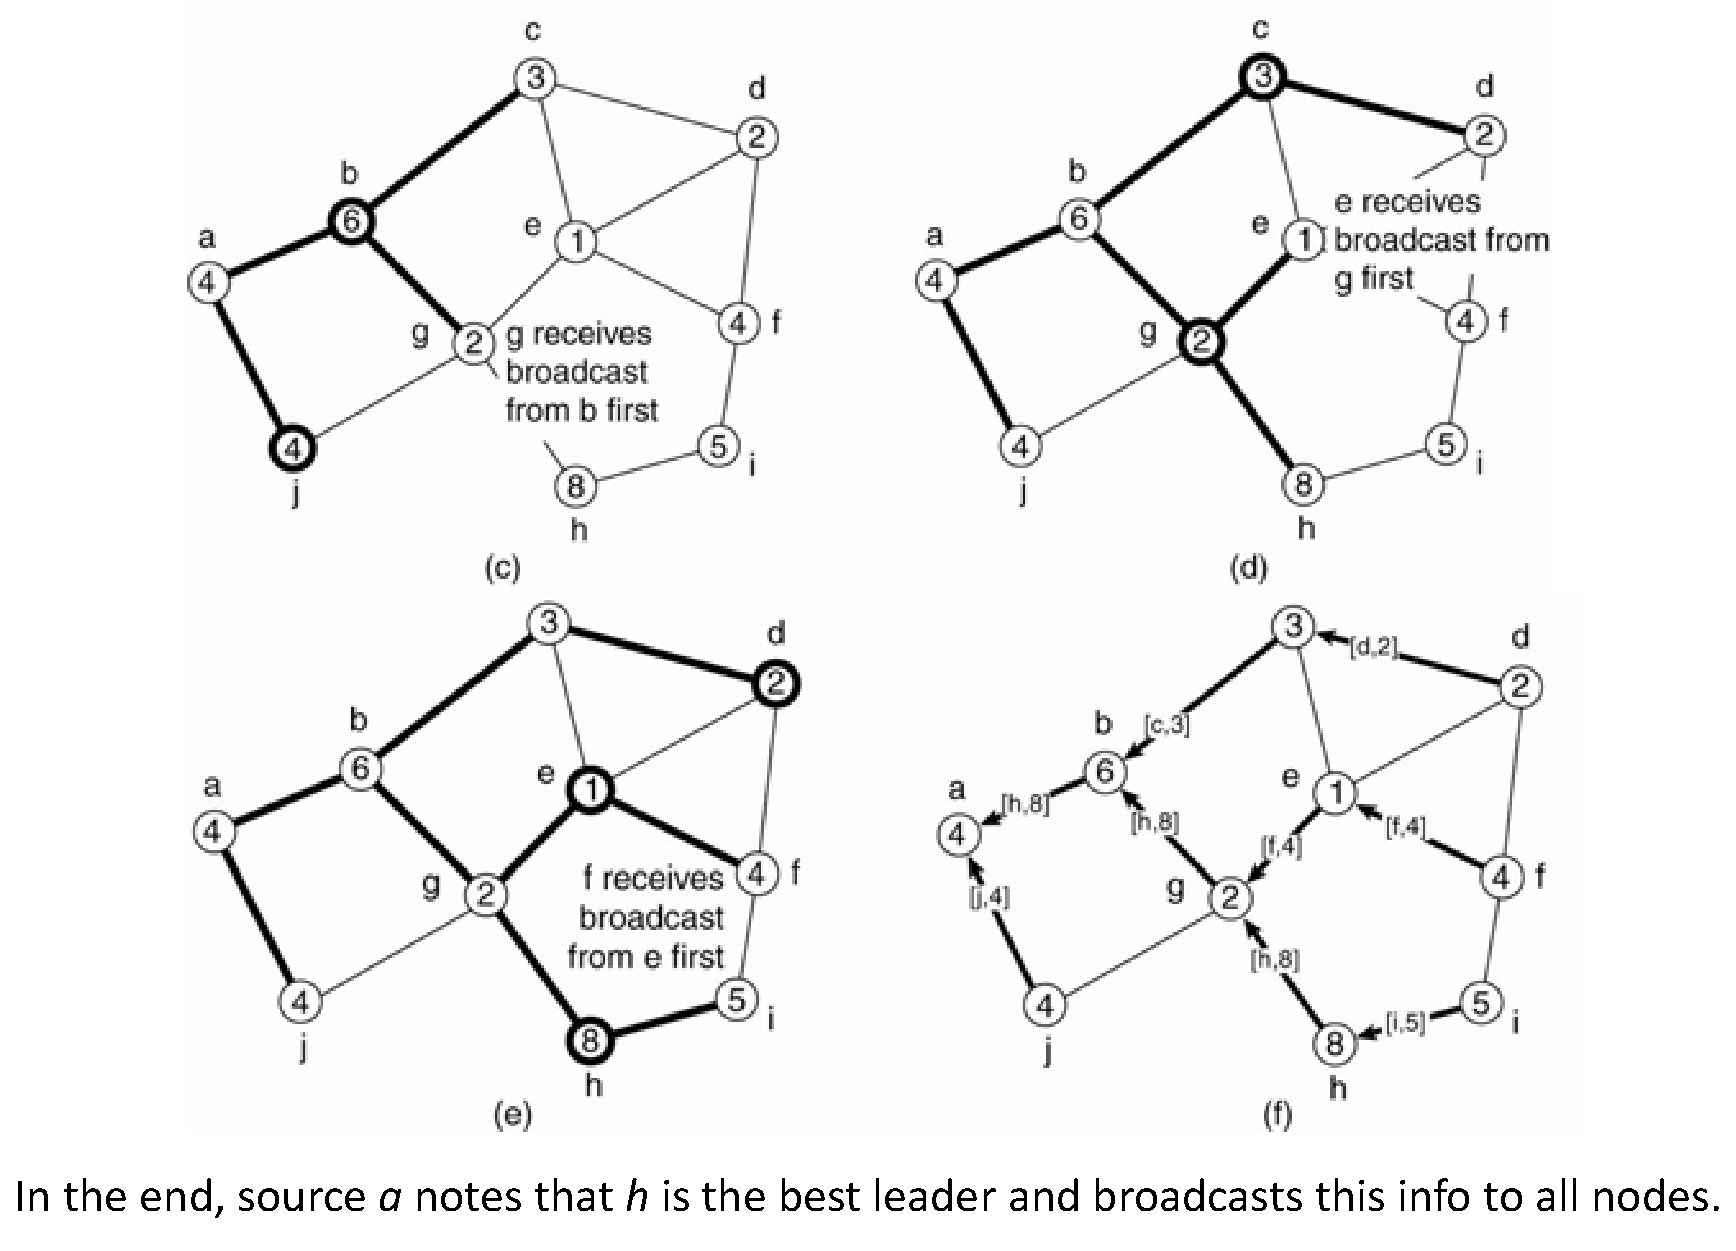
\includegraphics[width=1\linewidth]{pdi_1/example_general_topology_p2.pdf}
    \caption{Příklad činnosti algoritmu pro obecnou topologii, část 2.}
\end{figure}

\newpage

% VUT FIT MITAI
% MSZ 2021/2022
% Author: Vladimir Dusek
% Login: xdusek27

%%%%%%%%%%%%%%%%%%%%%%%%%%%%%%%%%%%%%%%%%%%%%%%%%%%%%%%%%%%%%%%%%%%%%%%%%%%%%%%%

\chapter{Podmínky konsistentního globálního stavu distribuovaného systému.}

% Todo:
% - Chtelo by to pravdepodobne doplnit i algoritmy pro dosazeni konzistentniho stavu.

%%%%%%%%%%%%%%%%%%%%%%%%%%%%%%%%%%%%%%%%%%%%%%%%%%%%%%%%%%%%%%%%%%%%%%%%%%%%%%%%

\subsection*{Metadata}

\begin{compactitem}
    \item Předmět: Prostředí distribuovaných aplikací (PDI)
    \item Přednáška:
    \begin{compactitem}
        \item 4) Globální stav a snapshots
    \end{compactitem}
    \item Záznam:
    \begin{compactitem}
        \item 2020-10-12
    \end{compactitem}
\end{compactitem}

%%%%%%%%%%%%%%%%%%%%%%%%%%%%%%%%%%%%%%%%%%%%%%%%%%%%%%%%%%%%%%%%%%%%%%%%%%%%%%%%

\section{Úvod a kontext}

\paragraph*{Distribuovaný systém} Distribovaný systém je množina procesů $p_1, p_2, \dots, p_n$, které jsou propojeny komunikačními kanály. V systému neexistuje žádná globální paměť ani globální hodiny. Procesy spolu komunikují pouze zasíláním zpráv skrze komunikačními kanály.

\paragraph*{Komunikační kanál} Komunikační kanál mezi procesy $p_i$ a $p_j$ značíme $C_{ij}$.

\paragraph*{Událost} Rozlišujeme tři typy událostí: interní událost procesu, zaslání zprávy a přijetí zprávy.

\paragraph*{Zpráva} Zpráva $m_{ij}$ značí zprávu zaslanou procesem $p_i$ procesu $p_j$. $send(m_{ij})$ značí odeslání zprávy a $recv(m_{ij})$ přijetí.

\paragraph*{Stav procesu} Lokální stav procesu $p_i$ značíme $LS_i$. Lokální stav je definován jako sekvence všech událostí, o kterých proces $p_i$ ví. Nechť $e$ je libovolná událost, $e \in LS_i$ značí, že událost $e$ patří do lokálního stavu procesu $p_i$, $e \not\in LS_i$ značí, že událost $e$ nepatří do lokálního stavu procesu $p_i$.

\paragraph*{Stav komunikačního kanálu} Stav komunikačního kanálu $C_{ij}$ značíme $SC_{ij}$ a je definován množinou zpráv, které obsahuje. Pro kanál $C_{ij}$ můžeme definovat jeho stav na základě lokálních stavů procesů $LS_i$ a $LS_j$: $$
transit(LS_i, LS_j) = \{ m_{ij} \,|\, send(m_{ij}) \in LS_i \land rec(m_{ij}) \not\in LS_j \}
$$.

\section{Model komunikace}

\begin{compactitem}
    \item FIFO -- Komukační kanál funguje jako fronta zpráv \textit{first in}, \textit{first out}. Kanál tedy zachovává pořadí zpráv sám o sobě.

    \item non-FIFO -- Komunikační kanál se chová jako datová struktura množina, do které odesílatel vkládá zprávy a příjemce je odebírá v náhodném pořadí.

    \item Causal ordering (kauzální uspořádání) -- Systém, který podporuje kauzální doručení zpráv splňuje následující vlastnost. Pro jakékoliv dvě zprávy $m_{ij}$ a $m_{kj}$ platí, pokud $send(m_{ij}) \rightarrow send(m_{kj})$, pak i $recv(m_{ij}) \rightarrow recv(m_{kj})$.
\end{compactitem}

\section{Konzistentní globální stav}

\paragraph*{Globální stav} Globální stav distribuovaného systému je kolekce lokálních stavů procesů a komunikačních kanálů. $$
GS = \Big\{ \bigcup_{i} LS_i \,,\, \bigcup_{i, j} SC_{ij} \Big\}
$$.

\paragraph*{Časoprostorový diagram} Diagram pro vizualizaci komunikace procesů v distribuovaném systému. Viz obrázek~\ref{48_example_cut} a~\ref{48_example_consistent_state}.

\paragraph*{Konzistentní globální stav} Konzistentní globální stav (\textit{snapshot}) je stav systému v určitém časovém okamžiku. Lze si jej představit jako řez v časoprostorovém diagramu, který rozděluje diagram na dvě části: minulost a budoucnost. Aby byl řez (globální stav) konzistentní, tak pokud je doručení nějaké zprávy v minulosti, musí být v minulosti i její odeslání. Formálně jde o globální stav, který splňuje nálsedující podmínky:

$$
send(m_{ij}) \in LS_i \Rightarrow m_{ij} \in SC_{ij} \oplus recv(m_{ij}) \in LS_j
$$,

$$
send(m_{ij}) \not\in LS_i \Rightarrow m_{ij} \not\in SC_{ij} \land recv(m_{ij}) \not\in LS_j
$$.

\paragraph*{K čemu je \textit{snapshot}} \textit{Snapshot} lze využít např. pro tvorbu záloh systému nebo při zotavování systému po chybách.

\paragraph*{Jak lze \textit{snapshot} vytvořit} Absence globální sdílené paměti, globálních hodin a nepředvídatelná délka zpoždění v odesílání zpráv v distribuovaném systému činí problém vytváření snapshotů netriviálním. Způsob vytváření lze rozdělit do dvou kategorií: na základě algoritmů a na základě checkpointů.

\paragraph*{Problémy při zaznamenávání snapshotu} Jak rozlišit mezi zprávami, které mají být součástí snapshotu a které nikoliv?
\begin{compactitem}
    \item Zprávy, které jsou odeslány procesem před zaznamenáním svého  snapshotu, jsou zaznamenány do stavu.
    \item Zprávy, které jsouodeslány procesem po zaznamenání svého  snapshotu, nejsou zaznamenány do stavu.
\end{compactitem}

\noindent Jak rozpoznat okamžik, ve kterém má proces zaznamenat snapshot?
\begin{compactitem}
    \item Proces $p_j$ musí zaznamenat svůj snapshot před zpracováním zprávy $m_{ij}$, která byla poslána procesem $p_i$ po zaznamenání jeho snapshotu.
\end{compactitem}

\begin{figure}[H]
    \centering
    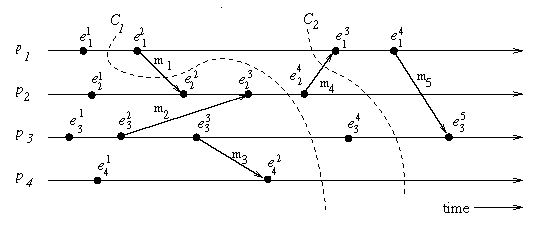
\includegraphics[width=1\linewidth]{pdi_2/example_cut.pdf}
    \caption{Příklad řezu v časoprostorovém diagramu. Řez $C_1$ je nekonzistentní, kvůli zprávě $m_1$. Řez $C_2$ je konzistentní a zpráva $m_4$ je zachycena ve stavu kanálu $Ch_{21}$.}
    \label{48_example_cut}
\end{figure}


\begin{figure}[H]
    \centering
    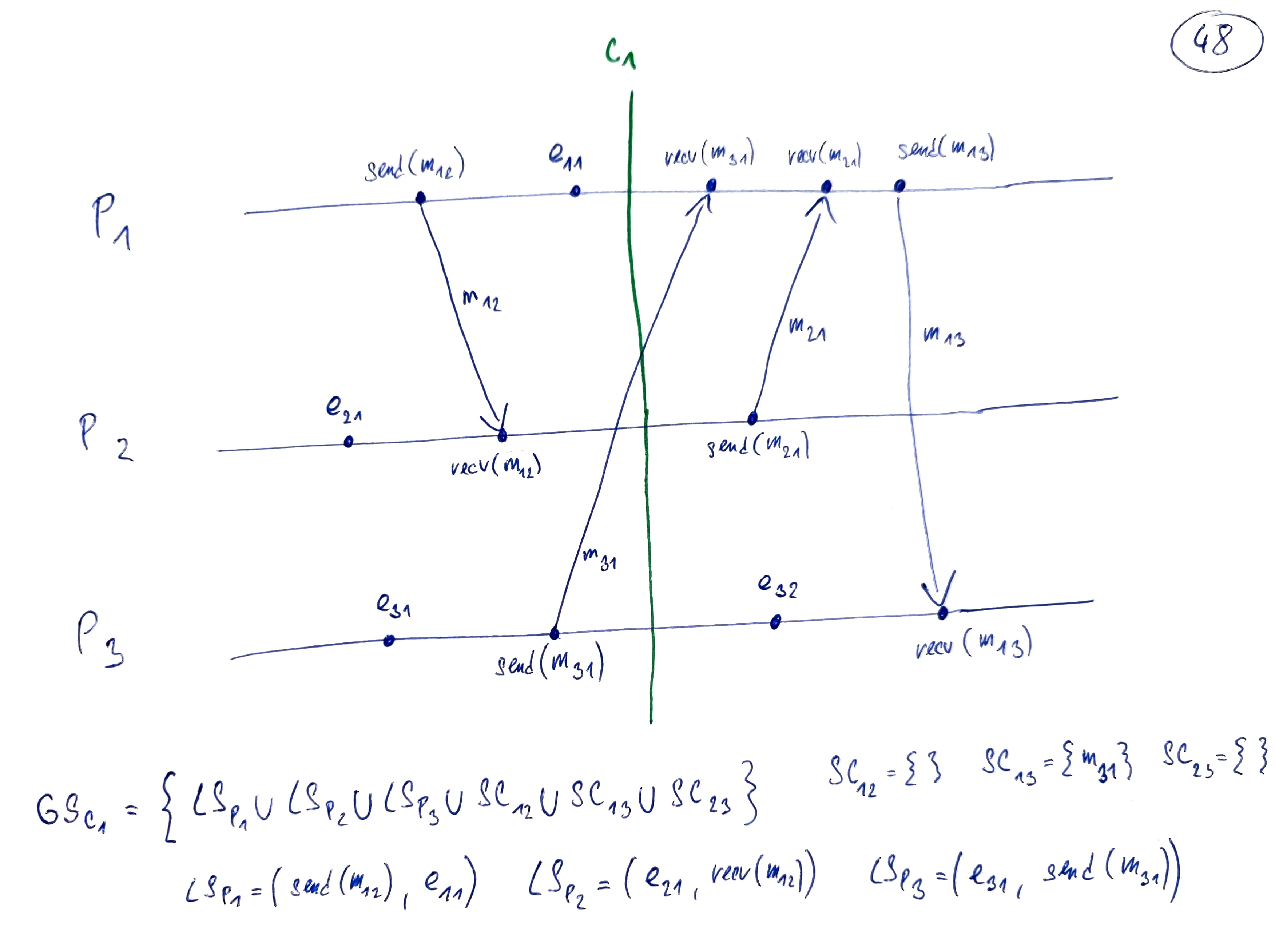
\includegraphics[width=1\linewidth]{pdi_2/example_consistent_state.pdf}
    \caption{Příklad konzistentního globální stavu formálně.}
    \label{48_example_consistent_state}
\end{figure}

\newpage

% VUT FIT MITAI
% MSZ 2021/2022
% Author: Vladimir Dusek
% Login: xdusek27

%%%%%%%%%%%%%%%%%%%%%%%%%%%%%%%%%%%%%%%%%%%%%%%%%%%%%%%%%%%%%%%%%%%%%%%%%%%%%%%%

\chapter{Principy distribuovaného zpracování MapReduce, průběh a jednotlivé operace distribuovaného výpočtu pomocí MapReduce, jeho implementace v Apache Hadoop a Apache Spark.}

%%%%%%%%%%%%%%%%%%%%%%%%%%%%%%%%%%%%%%%%%%%%%%%%%%%%%%%%%%%%%%%%%%%%%%%%%%%%%%%%

\section{Metadata}

\begin{compactitem}
    \item Předmět: Prostředí distribuovaných aplikací (PDI)
    \item Přednáška:
    \begin{compactitem}
        \item 9) Programovací model MapReduce a Apache Hadoop
        \item 10) Distribuované souborové systémy
        \item 11) Apache Spark
    \end{compactitem}
    \item Záznam:
    \begin{compactitem}
        \item 2020-11-16
        \item 2020-11-23
    \end{compactitem}
\end{compactitem}

%%%%%%%%%%%%%%%%%%%%%%%%%%%%%%%%%%%%%%%%%%%%%%%%%%%%%%%%%%%%%%%%%%%%%%%%%%%%%%%%

\section{Úvod a kontext}

\paragraph*{OLTP} OLTP (\textit{Online Transactional Processing}, provozní databáze, systémy pro online zpracování transakcí) jsou standardní databázové systémy s pevnou strukturou dat definovou pomocí databázového schématu. Jsou navrženy a optimalizovány pro chod provozních aplikací s primárním cílem zajistit rychlý a souběžný přístup k datům. To vyžaduje transakční zpracování, řízení souběžnosti a techniky obnovy (rollback), které zaručují konzistenci dat. Díky těmto vlastnostem mají OLTP databáze špatný výkon při provádění složitých dotazů, které potřebují spojit mnoho relačních tabulek dohromady nebo agregovat velké objemy dat. Kromě toho obsahují typicky podrobná data a neobsahují historická data, která jsou při datové analýze potřeba.

\paragraph*{OLAP} OLAP (\textit{Online Analytical Processing}, online analytické zpracování) je databázové paradigma specificky zaměřené na dotazy, zejména na analytické dotazy. Používají se zde jiné techniky indexování a optimalizace dotazů. Normalizace není pro toto paradigma žádoucí, protože rozděluje databázi na mnoho tabulek. Složité dotazy v takovém případě vyžadují rekonstrukci dat a s tím spojený vysoký počet spojování tabulek. Pracuje se s tzv. multidimenzionálními kostkami, avšak v pozadí jsou stále relační databáze.

\paragraph*{NoSQL} Potřeba ukládat proudy dat (zpracovávané v reálném čase bez možnosti pozastavení), obrázky, multimédia, velké JSON soubory, \dots, vedla ke vzniku NoSQL databází. NoSQL databáze používají jiné prostředky než tabulková schémata tradiční relační databáze. Často jde o \uv{hloupé}, nestrukturované uložiště klíč-hodnota.

\paragraph*{BigData} Velká, nestrukturovaná (různorodá), rychle rostoucí data, která není možné uložit ani zpracovávat běžnými přístupy (na jednom uzlu, jedním uzlem). Produkují je např.: IoT senzory, sociální sítě, chatovací aplikace, webové vyhledávače, \dots \, Pro jejich zpracování je nutné využít distribuované systémy (pro uložení i zpracování).

\paragraph*{Distribuované zpracování dat} Distribuované zpracování dat je zpracování velkých dat (\textit{big data}) pomocí distribuovaných systémů. To s sebou přináší problémy. Jak zaručit vhodnou distribuci dat a výpočtu mezi uzly? Jak řešit nespolehlivost a výpadky uzlů? Jak a kam zajistit doručení výsledků výpočtu? \dots

%%%%%%%%%%%%%%%%%%%%%%%%%%%%%%%%%%%%%%%%%%%%%%%%%%%%%%%%%%%%%%%%%%%%%%%%%%%%%%%%

\section{MapReduce}

Algoritmy pro indexování webových stránek (Page Rank) přestávaly být udržitelné, bylo potřeba zvýšit jejich škálovatelnost. Google vydal příspěvek \uv{MapReduce: Simplified Data Processing on Large Clusters}, kde bylo představeno paradigma MapReduce. Jde o paradigma distribuovaného výpočtu založené na funkcích \textit{map} a \textit{reduce} z funcionálního programování.

\paragraph*{Map} Funkce \textit{map} má ve funkcionálním programování 2 vstupní parametry a vrací seznam hodnot. První parametr je unární operátor (nebo funkce fungující jako unární operátor) a druhý je seznam hodnot. Výstupní seznam je spočítán jako aplikace unárního operátoru na vstupní seznam. Příklad:
$$
map(square, [1, 2, 3, 4]) = [1, 4, 9, 16]
$$.
V paradigmata MapReduce \textit{map} vrací data jako seznam dvojic klíč-hodnota, přesněji: $$
map((key, value)) \rightarrow [(key, value)]
$$.

\paragraph*{Reduce} Funkce \textit{reduce} má ve funkcionálním programování 2 vstupní parametry a vrací jednu hodnotu. První parametr je binární operátor (nebo funkce fungující jako binární operátor) a druhý je seznam hodnot. Výstupní hodnota je spočítána jako postupná aplikace binárního operátoru na všechny hodnoty ve vstupním seznamu. Příklad:
$$
reduce(+, [1, 4, 9, 16]) = 30
$$.
V paradigmata MapReduce \textit{reduce} bere na vstupu klíč a seznam hodnot a vrací opět seznam dvojic klíč-hodnota, přesněji: $$
reduce(key, [value]) \rightarrow [(key, value)]
$$.

\bigskip\noindent\begin{minipage}{\linewidth}
\begin{lstlisting}[language=Python, caption={Příklad implementace funkcí \textit{map} a \textit{reduce} v paradigmatu MapReduce pro počítání četnosti slov ve vstupu v Pythonu.}]
def map(input_key: str, input_value: str) -> list[tuple[str, int]]:
    # input_key - document name
    # input_value - document content (etc. line)
    result = []
    for word in input_value.split(' '):
        result.append((word, 1))
    return result

def reduce(input_key: str, input_value: list[int]) -> tuple[str, int]:
    result = 0
    for val in input_value:
        result += value
    return (input_key, result)
\end{lstlisting}
\end{minipage}

\begin{figure}[H]
    \centering
    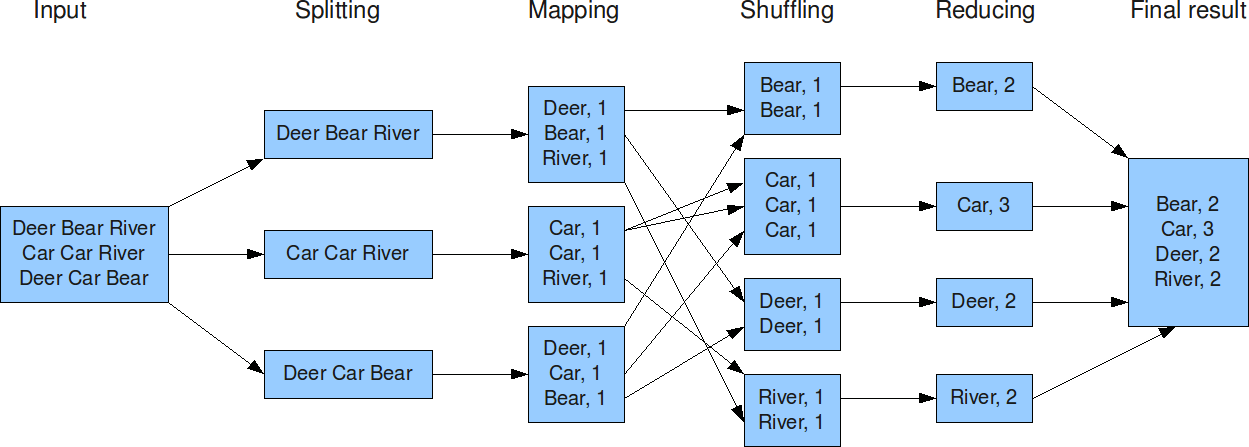
\includegraphics[width=1\linewidth]{pdi_3/map_reduce_example.png}
    \caption{Úloha počítání četnosti slov v paradigmatu MapReduce v diagramu.}
    \label{49_map_reduce_example}
\end{figure}

\paragraph*{Průběh MapReduce} Celý MapReduce probíhá v několika krocích, viz obrázek~\ref{49_map_reduce_example}.
\begin{compactenum}
    \item Input -- Přípravený vstup pro distribuovaný výpočet (např. soubory ve virtuálním distribuovaném souborovém systému, viz dále HDFS).
    \item Splitting -- Rozdělení vstupu na části, které budou přiděleny jednotlivým uzlům. Může být výchozí (např. rozdělení textového souboru po řádcích) nebo definováno uživatelem.
    \item Mapping -- Každý uzel aplikuje funkci \textit{map} na svoji přidělenou část. Uživatel definuje jak má funkce \textit{map} vypadat.
    \item Shuffling (také Grouping, Partitioning, Comparing)-- Výpočetní uzly si mezi sebou vymění hodnoty, které spočítaly, na základě klíče. Tento krok zařižuje platforma pro distribuovaný výpočet sama o sobě, typicky na základě hashů klíčů. Tento krok je většinou \textit{bottleneck}.
    \item Reducing -- Každý uzel zapojený do tohoto kroku (často je v tomto kroku potřeba méně uzlů, než v kroku mapping) aplikuje funkci \textit{reduce} na svoji přidělenou část. Uživatel definuje jak má funkce \textit{reduce} vypadat.
    \item Final Result -- Finální výsledek (např. zapsán do do virtuálního distribuovaného souborového systému, viz dále HDFS).
\end{compactenum}

\begin{figure}[H]
    \centering
    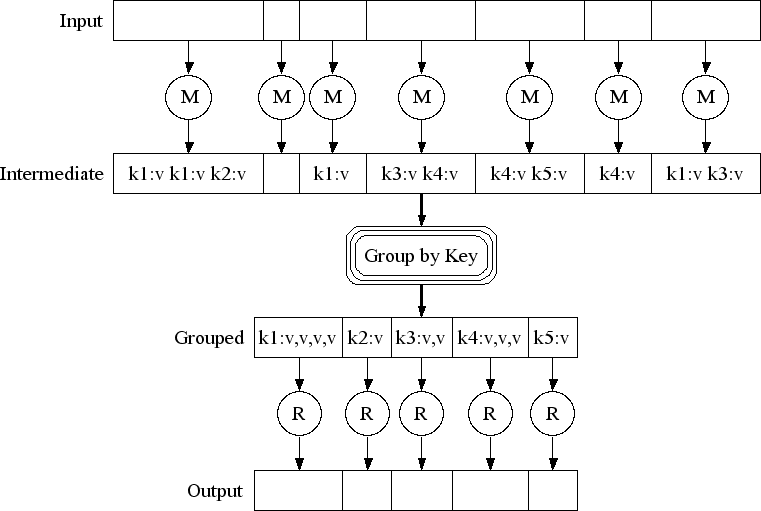
\includegraphics[width=1\linewidth]{pdi_3/map_reduce_general_p1.png}
    \caption{Výpočet MapReduce v obecném schématu.}
\end{figure}

\paragraph*{Combiner} Optimalizační krok, jde o \uv{jakési} provedení operace \textit{reduce} už ve fázi \textit{map} (každým uzlem). Tím je snížen počet mezivýsledků ve fázi Shuffling. Typicky funkce \textit{combine} je stejná jako \textit{reduce}.

\paragraph*{Virtuální distribuovaný souborový systém} Pro realizaci distribuovaného výpočtu je rovněž potřeba distribuovaný souborový systém (DFS). Ten je typicky realizován jako virtuální souborový systém nad jednotlivými souborovými systémy uzlů. Např.: GFS -- Google File System, HDFS -- Hadoop File System (viz dále). DFS obsahuje data samotná (\textit{data nodes}) a metadata o tom, která data jsou na jakých uzlech (\textit{name nodes}).

\begin{figure}[H]
    \centering
    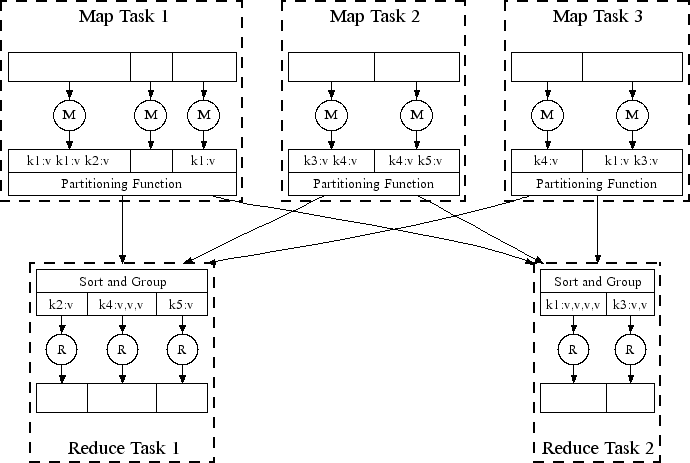
\includegraphics[width=1\linewidth]{pdi_3/map_reduce_general_p2.png}
    \caption{Výpočet MapReduce v obecném schématu a rozdělením práce na jednotlivé uzly (uzel je typicky víceprocesorový).}
\end{figure}

%%%%%%%%%%%%%%%%%%%%%%%%%%%%%%%%%%%%%%%%%%%%%%%%%%%%%%%%%%%%%%%%%%%%%%%%%%%%%%%%

\section{Apache Hadoop}

% Todo:
% - Dale by se dalo mluvit podrobneji o implementaci, viz slajd 26 (job tracker, task tracker).

Apache Hadoop je \textit{open-source} implementace MapReduce paradigmatu vyvíjená Apache Software Foundation. Jde o implementaci v Jave, ta je vhodná, jelikož díky JVM (Java Virtual Machine) je spouštění uživatel definovaných funkcí \textit{map} a \textit{reduce} snadné.

\paragraph*{Hadoop MapReduce} -- Implementace MapReduce paradigma. Data jsou čtena a ukládána na HDFS (včetně mezivýsledků). To znamená, můžeme pracovat v podstatě neomezenými daty, ale ukládání a načítání výpočet zpomalují.\footnote{\textit{Nebylo přednášeno podrobněji, pravděpodobně stačí princip obecného MapReduce, který byl vysvětlen v předchozí sekci.}}.

\paragraph*{HDFS} HDFS (\textit{Hadoop Distribute File System}) je virtuální distribuovaný souborový systém. Standardní soubor je rozdělen na datové bloky které jsou distribuovány na různé datové uzly. Architektura HDFS se skládá ze dvou typů uzlů~--~Name Node a Data Node. Name Node obsahuje alokační tabulku pro souborový systém. Ví které datové bloky patří kterému souboru a kde jsou uloženy. Obsahuje další metadata jako názvy souborů, cesty, \dots \, Data Node obsahuje datové bloky. Typicky redundance a replikace, počítá se s možným selháním uzlů. Pro \textbf{čtení dat} se klient zeptá Name Nodu na konkrétní soubor v HDFS. Name Node vrátí metadata o souboru, na jakých Data Nodech se vyskytuje. Klient požádá příslušné Data Nody, ty mu pošlou data, která se na klientovi \uv{poskládají} do výsledného souboru. Pro \textbf{zápis dat} se klient zeptá Name Nodu, kam by měl zapisovat. Klient zapíše na příslušný Data Node. Data Node poté vyřeší replikace s dalšími uzly.

\paragraph*{Hadoop YARN} Hadoop YARN je plánovač (\textit{scheduler}). Plánuje výpočet tak, aby proběhl co nejlepším způsobem na konkrétnbí distribuované architektuře. Plánovač má obecné obecné rozhraní a Hadoop YARN lze nahradit za jiný.

\paragraph*{Hadoop Common} Hadoop Common jsou další knihovny a ovladače pro klienty.

\paragraph*{Další nástroje} Nad Apache Hadoop existuje mnoho dalších nástrojů. Apache Pig pro \textit{high level} programování map-reduce úloh. Apache Hive pro pro dolování dat nad Apache Hadoop. Apache HBase jako distribuovaná databáze nad Apache Hadoop, \dots

%%%%%%%%%%%%%%%%%%%%%%%%%%%%%%%%%%%%%%%%%%%%%%%%%%%%%%%%%%%%%%%%%%%%%%%%%%%%%%%%

\section{Apache Spark}

Apache Spark je \textit{open-source} nástroj pro distribuované zpracování rozsáhlých dat vyvíjený Apache Software Foundation. Hlavní cíl je zvýšení rychlosti. Spark na to jde přesunutím co nejvíce výpočtů do operační paměti jednotlivých uzlů a tím pádem zminimalizovat počet zápisů a čtení z DFS (snaha odstranit \textit{bottleneck} v kroku shuffling u Hadoopu). Tím ale vzniká jiný problém, a sice výpadek uzlu znamená, že data jsou ztraceny.

\begin{figure}[H]
    \centering
    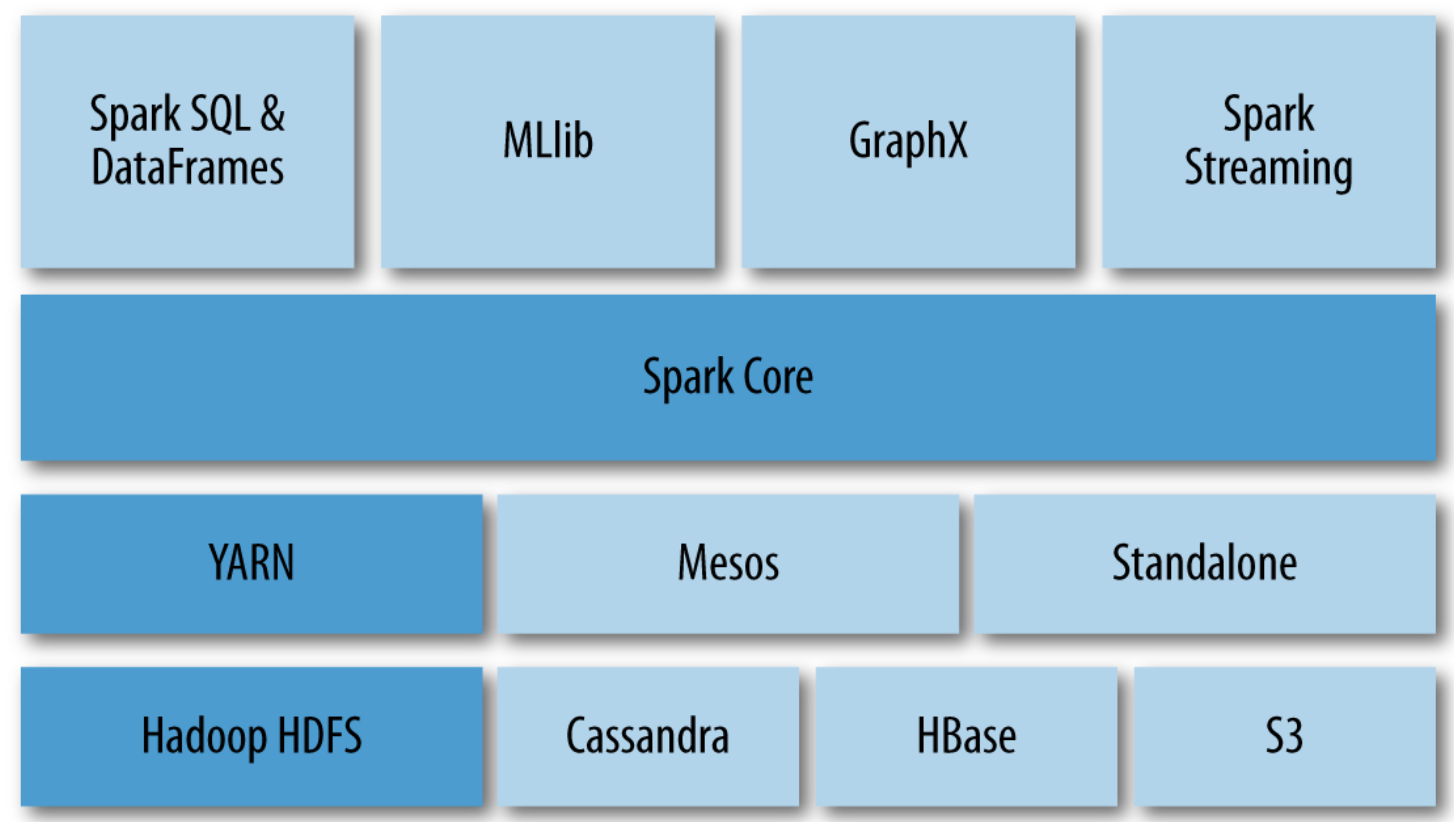
\includegraphics[width=0.75\linewidth]{pdi_3/spark.png}
    \caption{Architektura Apache Spark. Hlavní je Spark Core, zbytek funguje na systému pluginů a může používat HDFS, Hadoop YARN a Hadoop Common.}
\end{figure}

% todo: pokracovani, 30 min prednaska

\paragraph*{Resilient Distributed Dataset} Resilient Distributed Dataset (RDD) je základní datová struktura Sparku. Jedná se o typované kolekce n-tic, které jsou neměnné (\textit{read only}). Vstup je transformován na RDD a každá operace je pak transformace jednoho RDD na jiné.
$$
RDD_1 \rightarrow map() \rightarrow RDD_2 \rightarrow reduce() \rightarrow RDD_3
$$

\paragraph*{Strategie vyhodnocování} Spark uplatňuje strategii vyhodnocování \textit{lazy evaluation}. Vyhodnocování výrazu je odkládáno až do doby, dokud není potřeba jeho hodnota. Zabraňuje opakovanému vyhodnocování. Je vyhodnocována pouze ta část, která je potřeba. RDD funguje jako abstraktní datová struktura, nemusí obsahovat data uvnitř, ale pouze předpis jak data získat a získá je, až když jsou potřeba.

\paragraph*{Struktura výpočtu} Struktura výpočtu odpovídá orientovanému acyklickému grafu (DAG, \textit{Directed Acyclic Graph}). Uzly jsou RDD a hrany jsou transformace. DAG je znám i dalším uzlům, takže pokud nastane výpadek uzlu a výpočet je ztracen, může být uzel snadno zastoupen.

\paragraph*{Klíčové vlastnosti} Klíčové vlastnosti Sparku jsou \textit{lazy evaluation}, \textit{in-memmory} a \textit{parallel computing}.

\begin{figure}[H]
    \centering
    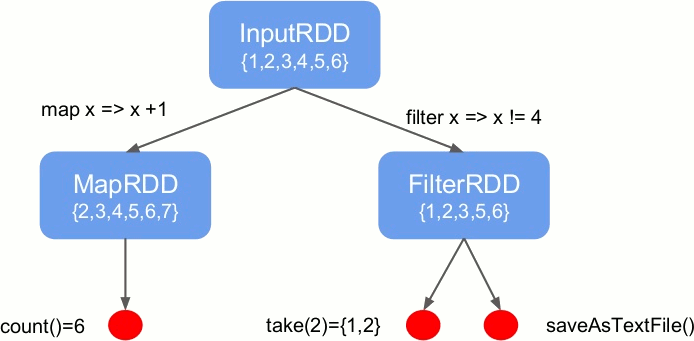
\includegraphics[width=0.85\linewidth]{pdi_3/spark_example.png}
    \caption{Příklad výpočtu v Apache Spark.}
\end{figure}

\newpage

% VUT FIT MITAI
% MSZ 2021/2022
% Author: Vladimir Dusek
% Login: xdusek27

%%%%%%%%%%%%%%%%%%%%%%%%%%%%%%%%%%%%%%%%%%%%%%%%%%%%%%%%%%%%%%%%%%%%%%%%%%%%%%%%

\chapter{Symetrická kryptografie. Vlastnosti, vlastnosti bezpečného algoritmu, délka klíče, útok silou,
příklady symetrických algoritmů, Feistelovy šifry, DES, režimy činnosti, proudové šifry.}

%%%%%%%%%%%%%%%%%%%%%%%%%%%%%%%%%%%%%%%%%%%%%%%%%%%%%%%%%%%%%%%%%%%%%%%%%%%%%%%%

\section{Metadata}

\begin{compactitem}
    \item Předmět: Kryptografie (KRY)
    \item Přednáška:
    \begin{compactitem}
        \item 3) Symetrická kryptografie. Vlastnosti, vlastnosti bezpečného algoritmu, délka klíče, útok silou.
        \item 4) Příklady symetrických algoritmů, Feistelovy šifry, DES, struktura, činnost, slabiny, režimy činnosti.
        \item 5) Typické aplikace symetrické kryptografie.
    \end{compactitem}
    \item Záznam:
    \begin{compactitem}
        \item 2021-02-22
        \item 2021-03-01
        \item 2021-03-08
    \end{compactitem}
\end{compactitem}

%%%%%%%%%%%%%%%%%%%%%%%%%%%%%%%%%%%%%%%%%%%%%%%%%%%%%%%%%%%%%%%%%%%%%%%%%%%%%%%%

\section{Úvod a kontext}

\paragraph*{Kryptografie} Kryptografie (šifrování) je věda o~metodách utajování smyslu zpráv převodem do podoby, která je čitelná jen se speciální znalostí.

\paragraph*{Kryptoanalýza} Kryptoanalýza je věda zabývající se metodami získávání obsahu šifrovaných informací bez přístupu k~tajným informacím, které jsou za normálních okolností potřeba, tzn. především k~tajnému klíči.

\paragraph*{Kryptologie} Jeden výraz pro kryptografii a kryptoanalýzu.

\paragraph*{Caesarova šifra} Princip Caesarovy šifry je založen na tom, že všechna písmena zprávy jsou během šifrování zaměněna za písmeno, které se abecedně nachází o~pevně určený počet míst dále (tj. posun je pevně zvolen). Caesarova šifra spadá do kategorie substitučních šifer (stejný znak je při více vyskytech vždy zašifrován na stejný znak).

\paragraph*{Vigenerova šifra} Rozšíření Caesarovy šifry, klíč je delší než 1 znak. Klíč je řetězec, který reprezentuje posuny. V~případě že vstup je delší než klíč, je klíč perioricky opakován. Vigenerova šifra spadá do kategorie polyalfabetických substitučních šifer (stejný znak může být při více výskytech zašifrován na jiný znak).

\paragraph*{Vernamova šifra (\textit{One Time Pad})} Vernamova šifra spadá do kategorie polyalfabetických substitučních šifer a je i dnes nerozluštitelná pokud: \begin{compactitem}
    \item klíč je delší než vstupní text,
    \item klíč se nepoužije opakovaně,
    \item klíč je náhodný.
\end{compactitem}

\begin{figure}[H]
    \centering
    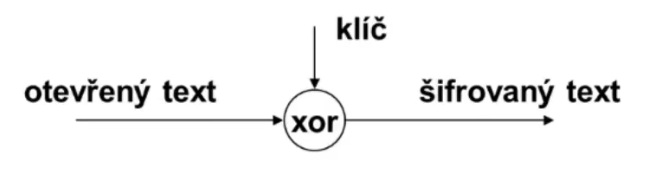
\includegraphics[width=0.5\linewidth]{kry_1/vernam.png}
    \caption{Vernamova šifra.}
\end{figure}

\paragraph*{Autoklíč (\textit{autokey})} Šifrování klíčem a když vstupní text je delší než klíč, tak se pokračuje šifrováním otevřeným nebo šifrovaným textem. Lze použít u~Vigenerovy nebo Vernamovy šifry.

\paragraph*{Symetrická kryptografie} Algoritmy používají k~šifrování i dešifrování stejný klíč. Výhodou symetrických šifer je jejich nízká výpočetní náročnost. Asymetrické šifry mohou být i stotisíckrát pomalejší. Nevýhodou je nutnost sdílení tajného klíče, takže jedna strana musí klíč vygenerovat a potom ho bezpečným způsobem předat druhé straně.

\paragraph*{Typy útoků} \begin{compactitem}
    \item Ciphertext Only Attack (COA) -- Útočník zná pouze zašifrovaný text a snaží se zjistit klíč nebo otevřený text. Nejčastěší případ.
    \item Known Plaintext Attack (KPA) -- Útočník zná zašifrovaný text a otevřený text a snaží se zjistit klíč.
    \item Chosen Plaintext Attack (CPA) -- Útočník zná to co v~KPA a navíc si text může zvolit.
\end{compactitem}

\paragraph*{Útok silou} Pří útoku silou (\textit{brute force}) zkouší útočník všechny teoreticky možné klíče, dokud nenajde ten správný.

\begin{figure}[H]
    \centering
    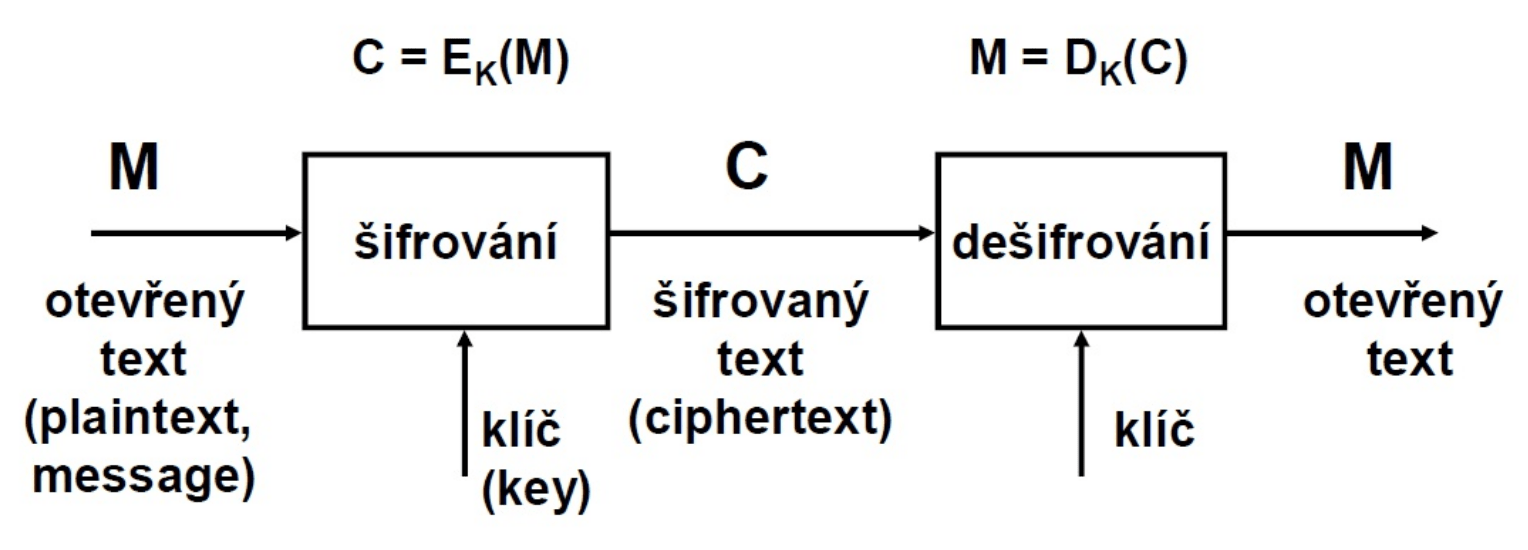
\includegraphics[width=0.75\linewidth]{kry_1/kryptografie.png}
    \caption{Princip kryptografie, podle typu klíčů dělíme na symetrickou (tajný klíč) a asymetrickou (veřejný klíč, soukromý klíč).}
\end{figure}

\paragraph*{Bezpečný algoritmus} V~moderní kryptografii je nepřijatelné utajování algoritmů (\textit{security by obscurity})~--~předpokládáme, že útočník zná šifrovací algoritmus. Bezpečnost musí záviset pouze na utajení klíče (Kerckhoffuv princip, \textit{security by design}). Symetrický algoritmus je považován za bezpečný, pokud neexistuje rychlejší útok než útok silou.

\paragraph*{Délka klíče} Dnes je považováno 80 bitů a více za dostatečné. Typicky se délka zaokrouhluje na mocninu 2 (typicky 128b). Klíče symetrických algoritmů jsou kratší než asymetrických. Konkrétně: DES -- 56b, 3DES -- 112, AES -- variabilní.

\paragraph*{Využití} Symetrická kryptografie je vhodná pro šifrování většího objemu dat. Narozdíl od asymetrické, která je pro tento účel příliš pomalá. Proto např. HTTPS využívá asymetrickou kryptografii pro výměnu symetrických klíčů a poté symetrickou kryptografii pro šifrování provozu.

\paragraph*{Vlastnosti moderní kryptografie} Symetrická kryptografie zaručuje všechny následující, kromě nepopiratelnosti~--~více entit má k~dispozici klíč. \begin{compactitem}
    \item Důvernost -- Utajení informace. Bez znalosti klíče, není možné data číst.

    \item Autentizace -- Prokázání, že zprávu skutečně poslal odesílatel a nikoliv útočník, který se za odesílatele vydává.

    \item Integrita -- Prokázání, že nikdo nemohl data po cestě od odesílatele k~příjemci změnit. Ochrana proti neoprávněné, neodhalené modifikaci zprávy.

    \item Nepopiratelnost -- Pokud odesílatel data poslal, nemůže tuto skutečnost popřít.
\end{compactitem}

%%%%%%%%%%%%%%%%%%%%%%%%%%%%%%%%%%%%%%%%%%%%%%%%%%%%%%%%%%%%%%%%%%%%%%%%%%%%%%%%

\section{Blokové šifry}

Blokové šifry šifrují data po blocích pevně stanovené délky (64b, 128b, 256b, \dots). Pokud je dat více, rozdělí se na více bloků, přičemž do zbylého místa v~posledním je umístěno zarovnání \textit{padding} (informace o~délce zarovnání může být obsažena v~posledním bytu). Příklady blokových šifer: \begin{compactitem}
    \item Feistelova šifra (spíše princip)
    \item Data Encryption Standard (DES)
    \item Triple Data Encryption Algorithm (3DES)
    \item International Data Encryption Algorithm (IDEA)
    \item Blowfish
    \item Tiny Encryption Algorithm (TEA)
    \item Advanced Encryption Standard (AES)
\end{compactitem}

\begin{figure}[H]
    \centering
    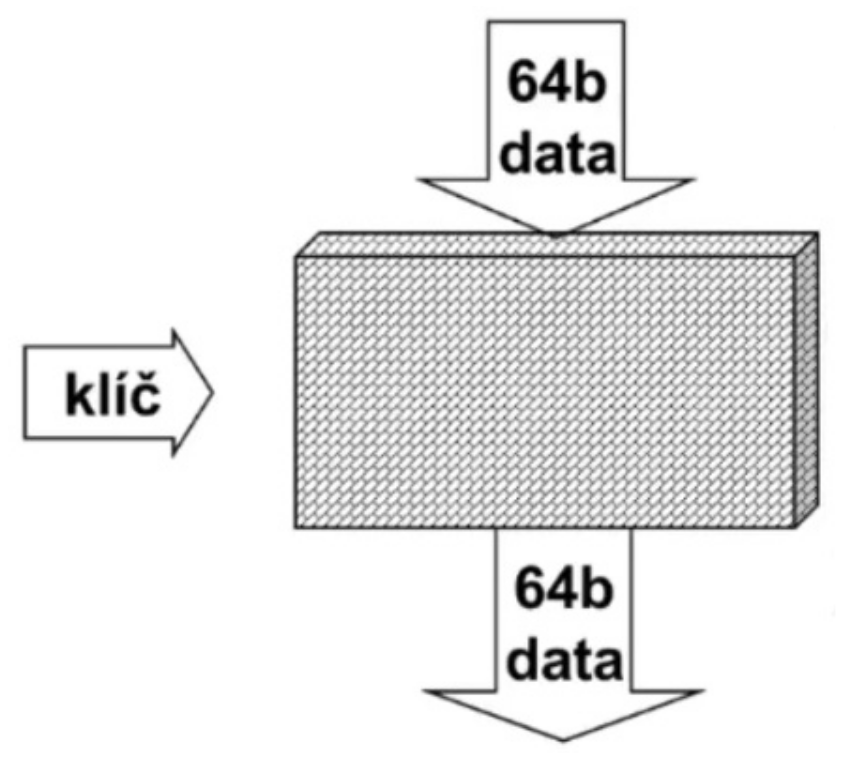
\includegraphics[width=0.35\linewidth]{kry_1/symmetric_cryptography_blocks.png}
    \caption{Princip blokových šifer.}
\end{figure}

\subsection*{Feistelova šifra}

Feistelova šifra (Feistelův princip) je koncept šifrování, který konkrétní algoritmy využívají. Jedná se o~substituční-permutační síť. Vstupní blok je rozdělen na dvě poloviny $L$ a $R$, výpočet výstupu pak vypadá následovně.

\begin{equation}
    L_i = R_{i-1}
\end{equation}

\begin{equation}
    R_i = L_{i-1} \oplus F(R_{i-1}, K_i)
\end{equation}

\paragraph*{Funkce F} $F$ je funkce, na kterou Feistelova šifra neklade žádné požadavky. Jednotlivé algoritmy, využívající Festelovu šifru, funkci samy definují. Požadavky na funkci $F$, aby algoritmus byl bezpečný: \begin{compactitem}
    \item skrytí vlastností zprávy;
    \item skrytí vlastností zprávy.
\end{compactitem}

\paragraph*{Subklíč} K~je tzv. subklíč, který je generován typicky nějakým pseudonáhodným generátorem na základě inicializačního klíče (hlavní).

\paragraph*{Dešifrování} Dešifrování se provádí stejným způsobem, pouze pořadí subklíčů je opačné.

\begin{figure}[H]
    \centering
    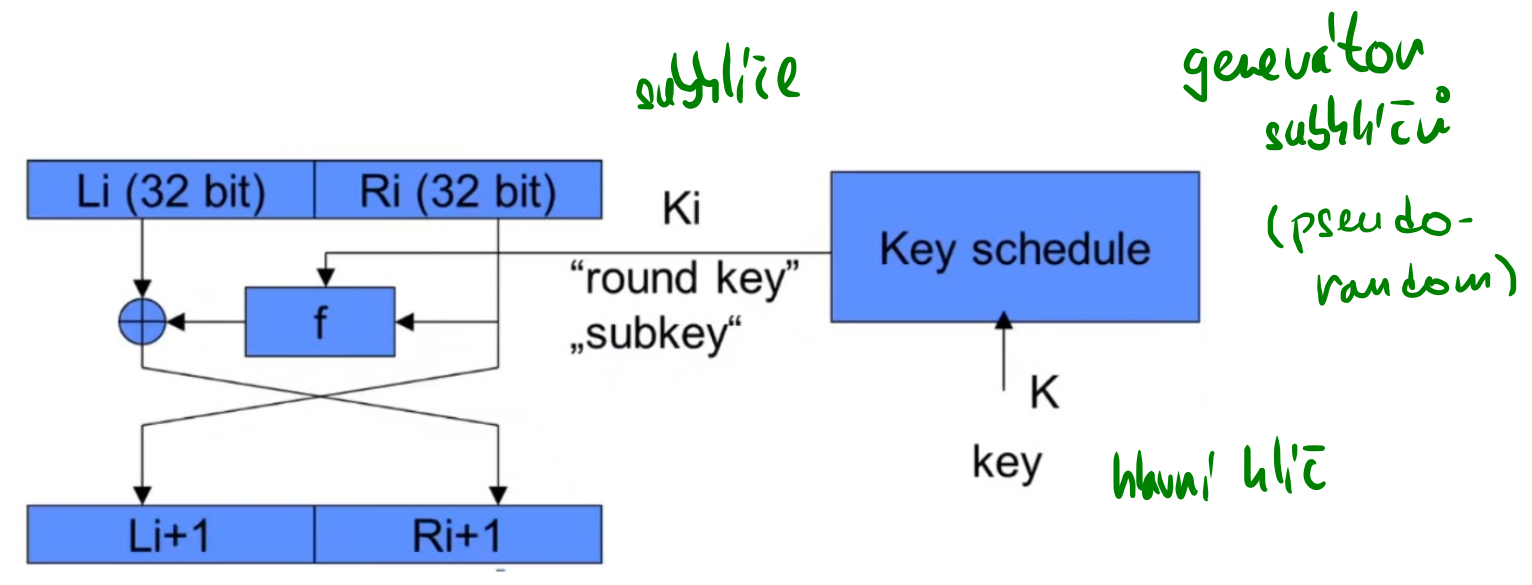
\includegraphics[width=1\linewidth]{kry_1/feistel.png}
    \caption{Jeden krok opakování (Feistelův krok) vizuálně.}
\end{figure}

\begin{figure}[H]
    \centering
    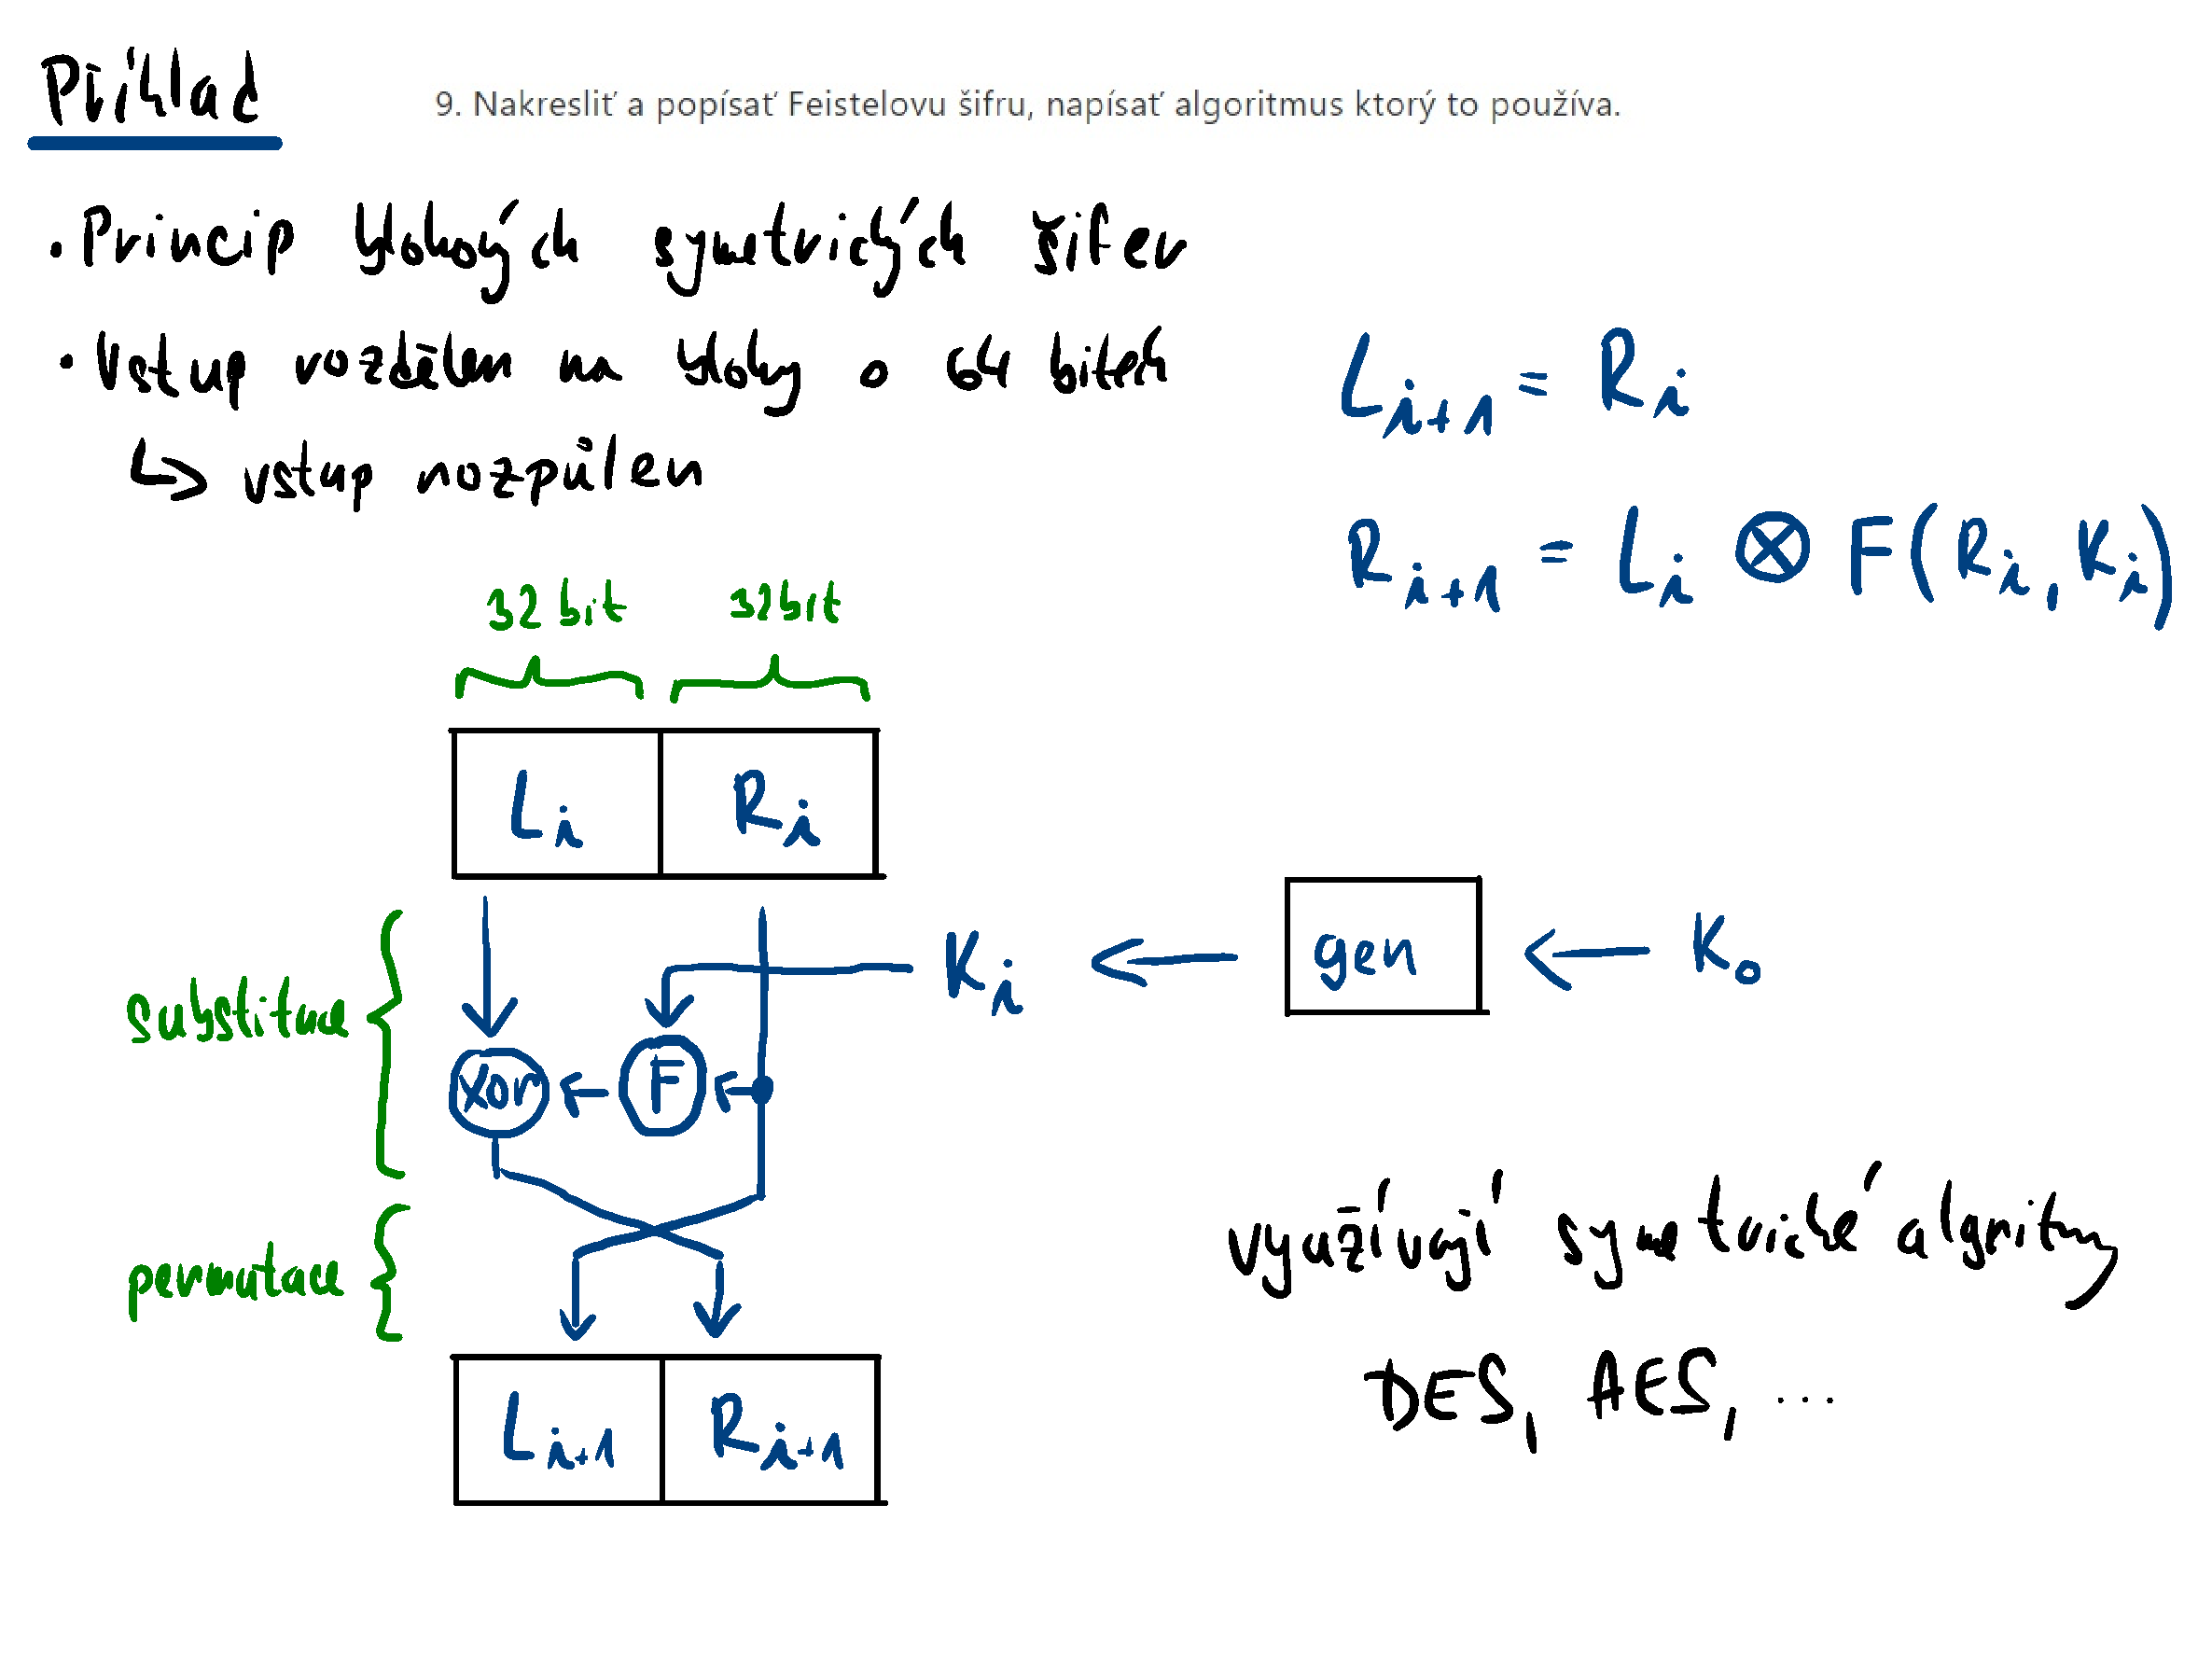
\includegraphics[width=1\linewidth]{kry_1/feistel_example.pdf}
    \caption{Feistelova šifra -- příklad a rekapitulace.}
\end{figure}

\subsection*{Data Encryption Standard (DES)}

DES byl první algoritmus s~veřejnou specifikací (\textit{security by design}). Využívá princip Feistelovy šifry -- 16 kol. Dodatečně přidává na začátek a konec permutaci navíc. Klíč je dlouhý 64b (resp. 56 významových bitů a 8 paritních).

\paragraph*{Slabiny} \begin{compactitem}
    \item 56 bitový klíč je příliš krátky a je možný útok silou.
    \item Rozdílná velikost bloku a klíče (zvláštnost).
    \item Existence slabých a poloslabých klíčů.
    \item Není jasné proč zrovna 16 iterací a zda je to dostatečné.
\end{compactitem}

\begin{figure}[H]
    \centering
    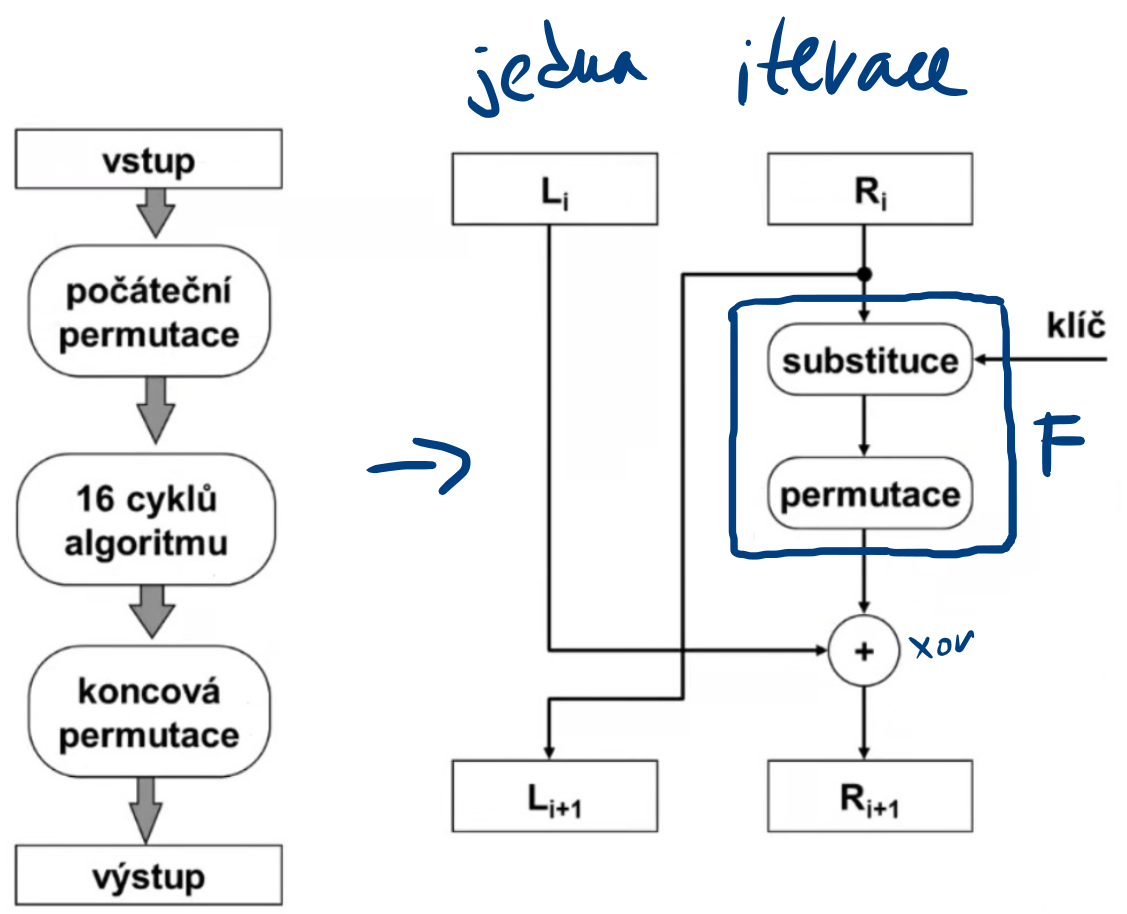
\includegraphics[width=0.75\linewidth]{kry_1/des_schema.png}
    \caption{DES -- Schéma fungování algoritmu.}
\end{figure}

\begin{figure}[H]
    \centering
    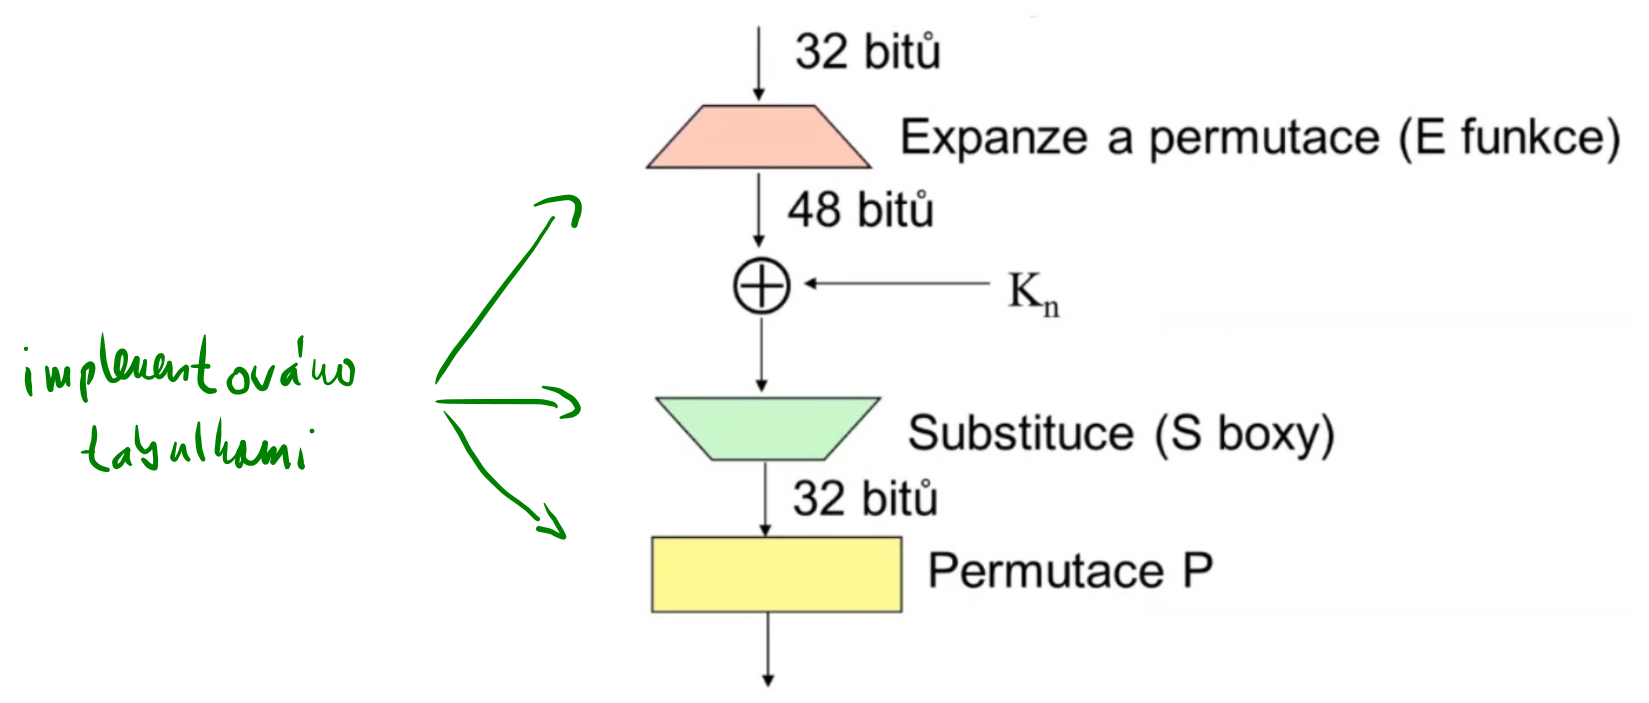
\includegraphics[width=1\linewidth]{kry_1/des_f.png}
    \caption{DES -- funkce F.}
\end{figure}

\begin{figure}[H]
    \centering
    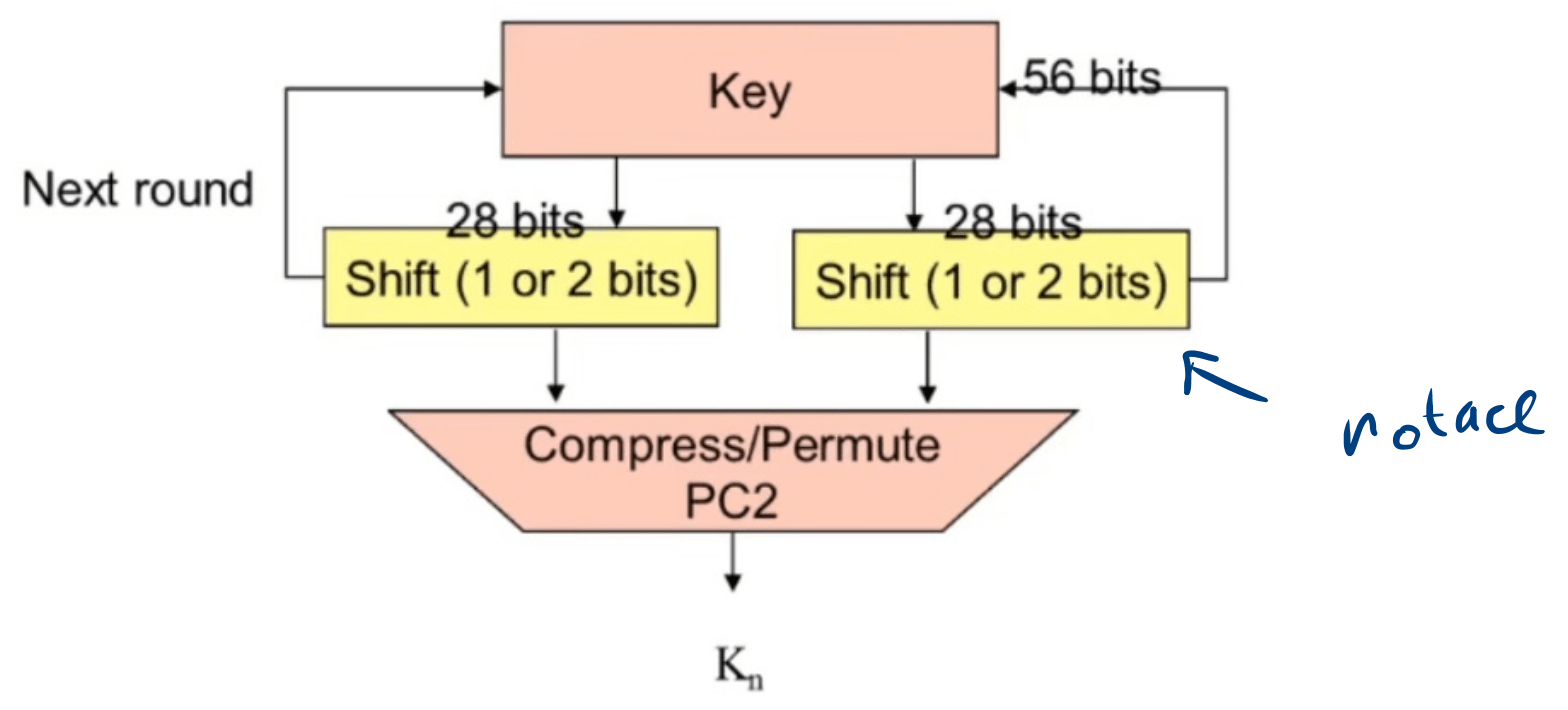
\includegraphics[width=1\linewidth]{kry_1/des_keys.png}
    \caption{DES -- generování subklíčů.}
\end{figure}

\begin{figure}[H]
    \centering
    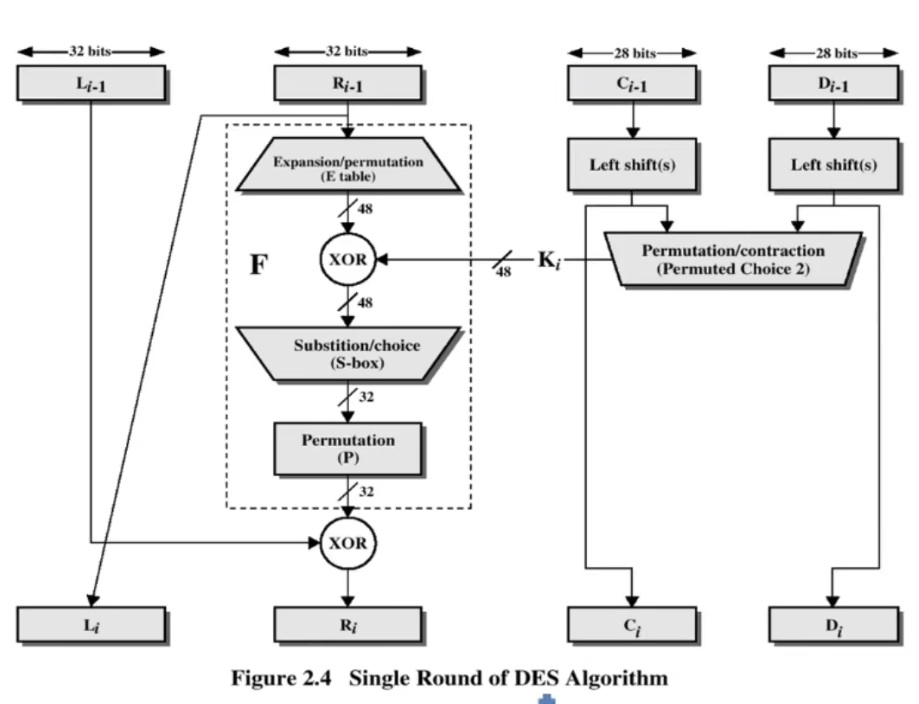
\includegraphics[width=1\linewidth]{kry_1/des_single_round.png}
    \caption{DES -- jedno kolo algoritmu. \textit{Left shift} je ve skutečnosti bitová rotace.}
\end{figure}

\begin{figure}[H]
    \centering
    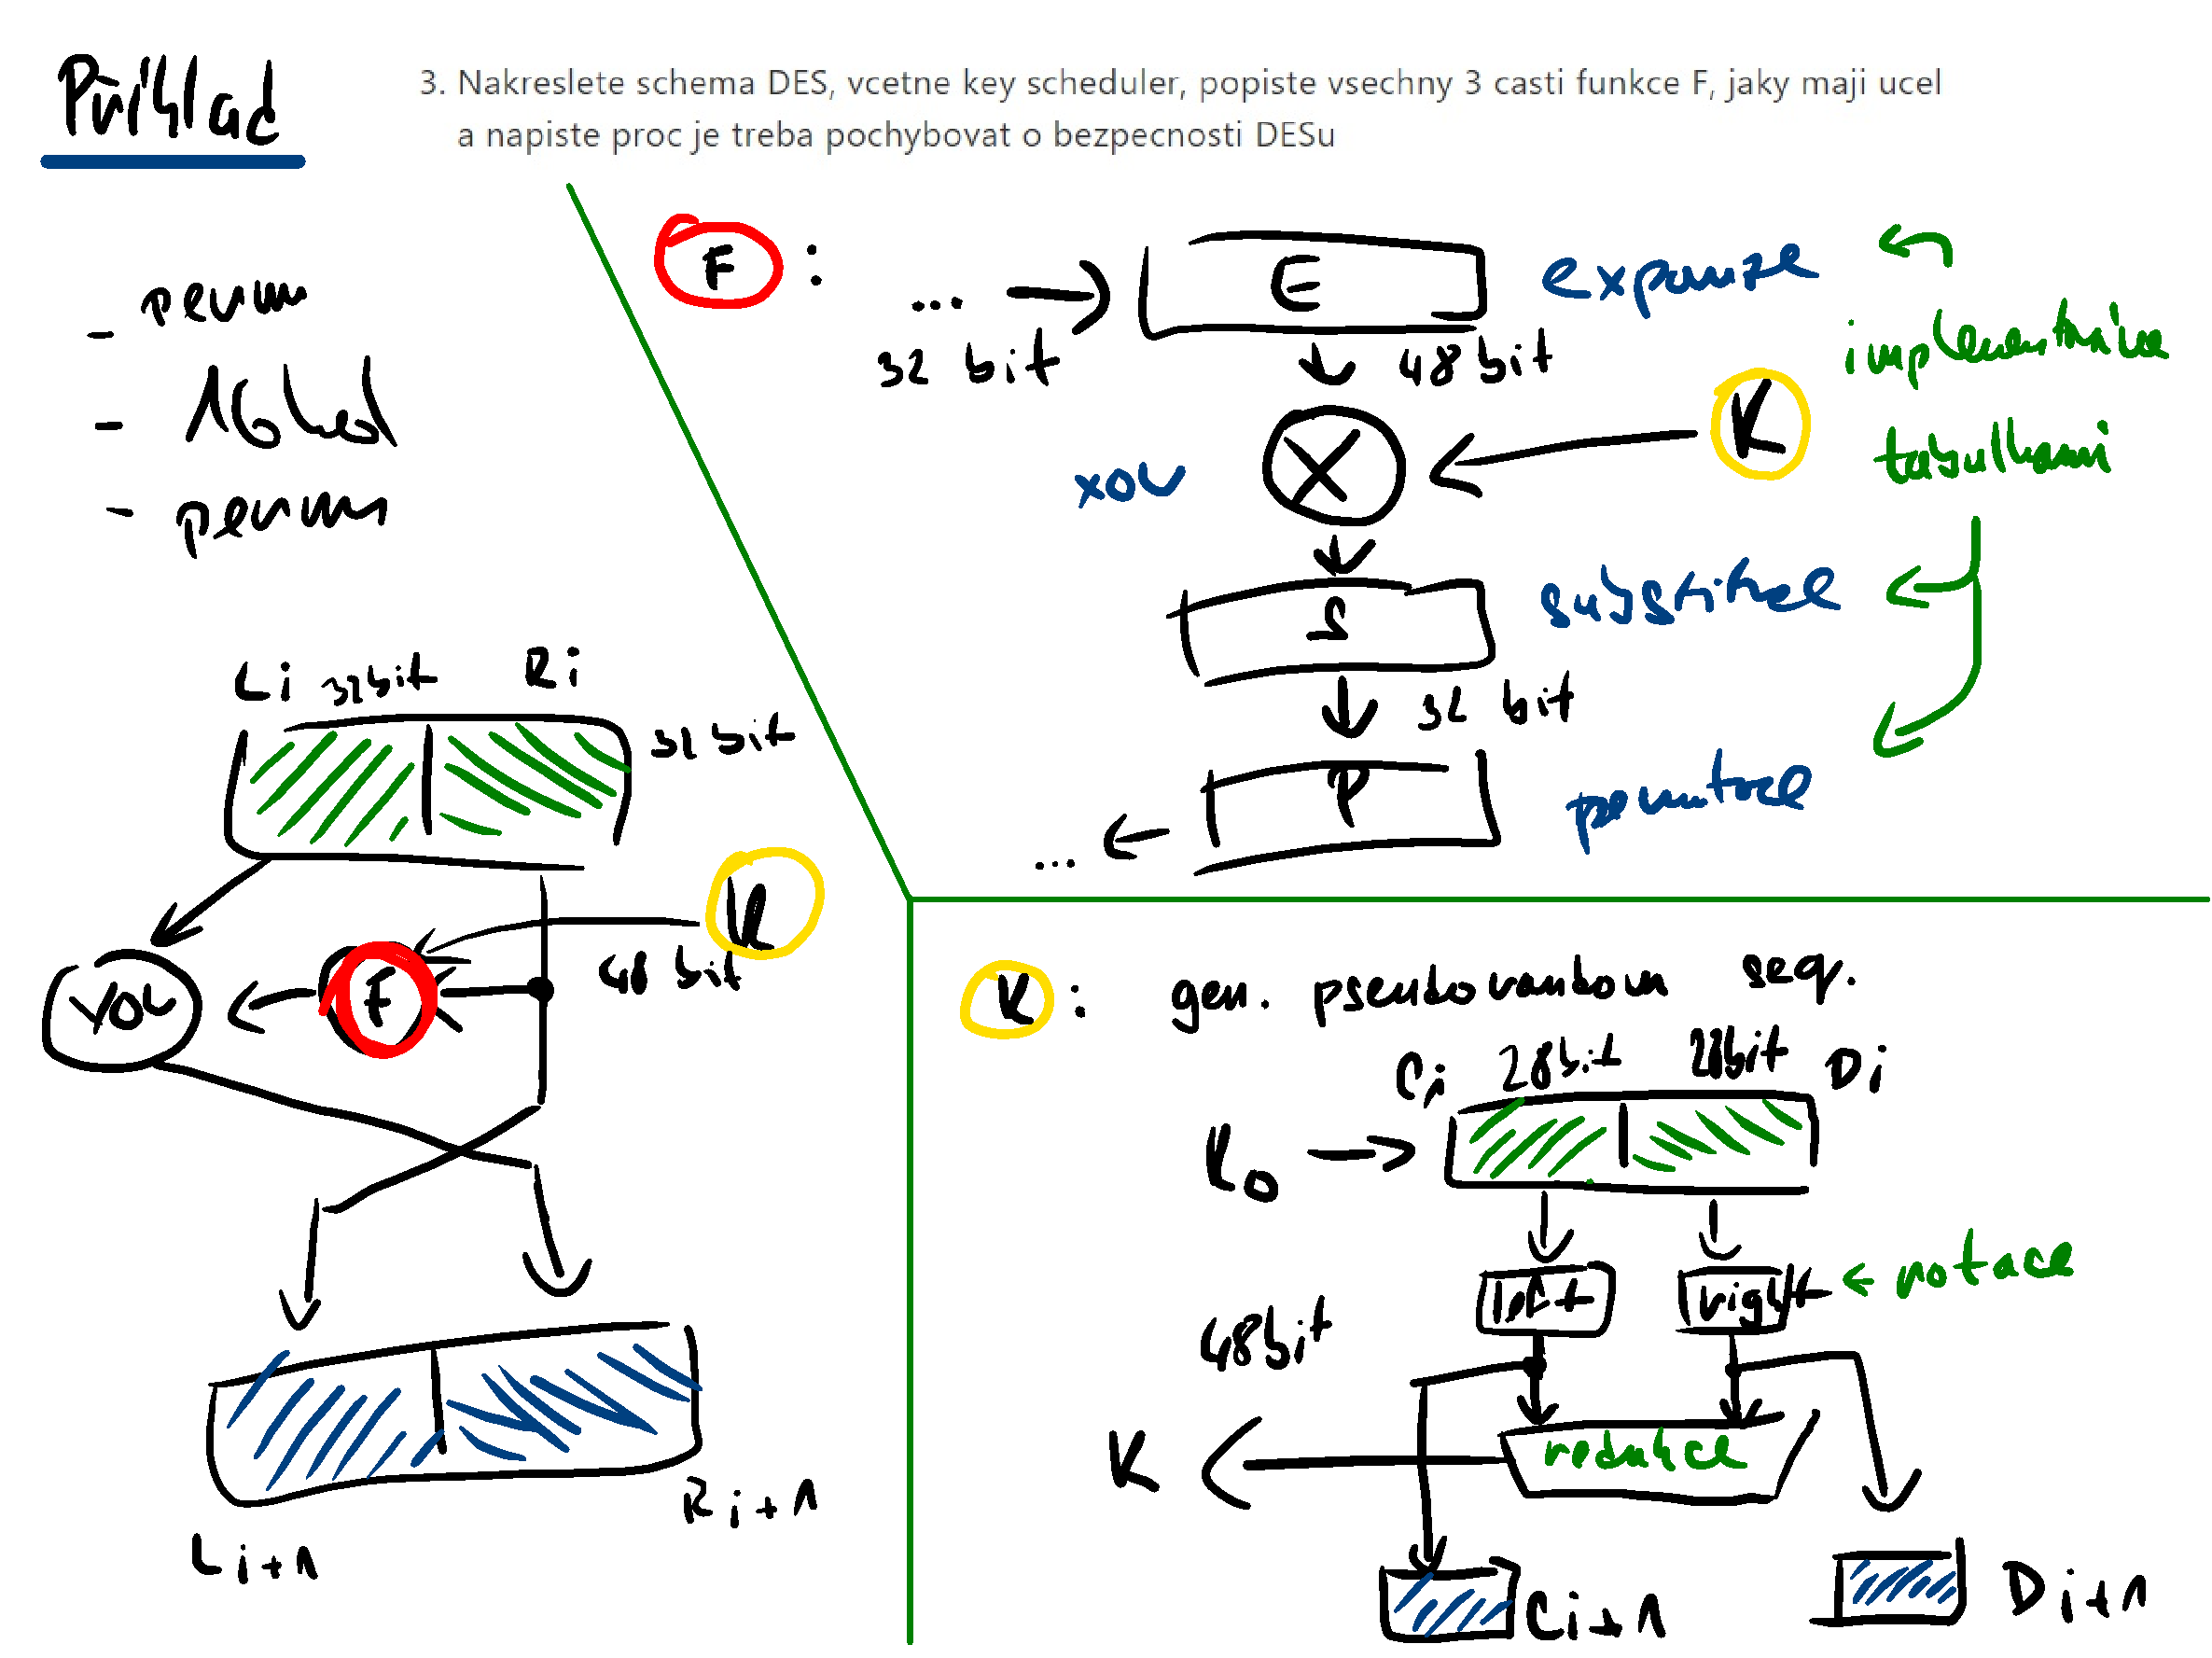
\includegraphics[width=1\linewidth]{kry_1/des_example.pdf}
    \caption{DES -- příklad a rekapitulace.}
\end{figure}

%%%%%%%%%%%%%%%%%%%%%%%%%%%%%%%%%%%%%%%%%%%%%%%%%%%%%%%%%%%%%%%%%%%%%%%%%%%%%%%%

\section{Provozní režimy činnosti blokových šifer}

Jak použít blokové šifry abychom byli schopni šifrovat data delší než jeden blok?

\subsection*{Electronic Code Book (ECB)}

ECB (\uv{kódová kniha}) je výchozí \textit{naivní} režim. Bloková šifra se při něm přímo aplikuje nezávisle na jednotlivé bloky, tedy při daném klíči odpovídá stejnému bloku otevřeného textu stejný blok šifrového textu. To má nežádoucí důsledky z~hlediska bezpečnosti, v~datech zůstane původní struktura, např. šifrovaný obrázek je rozpoznatelný.

\begin{figure}[H]
    \centering
    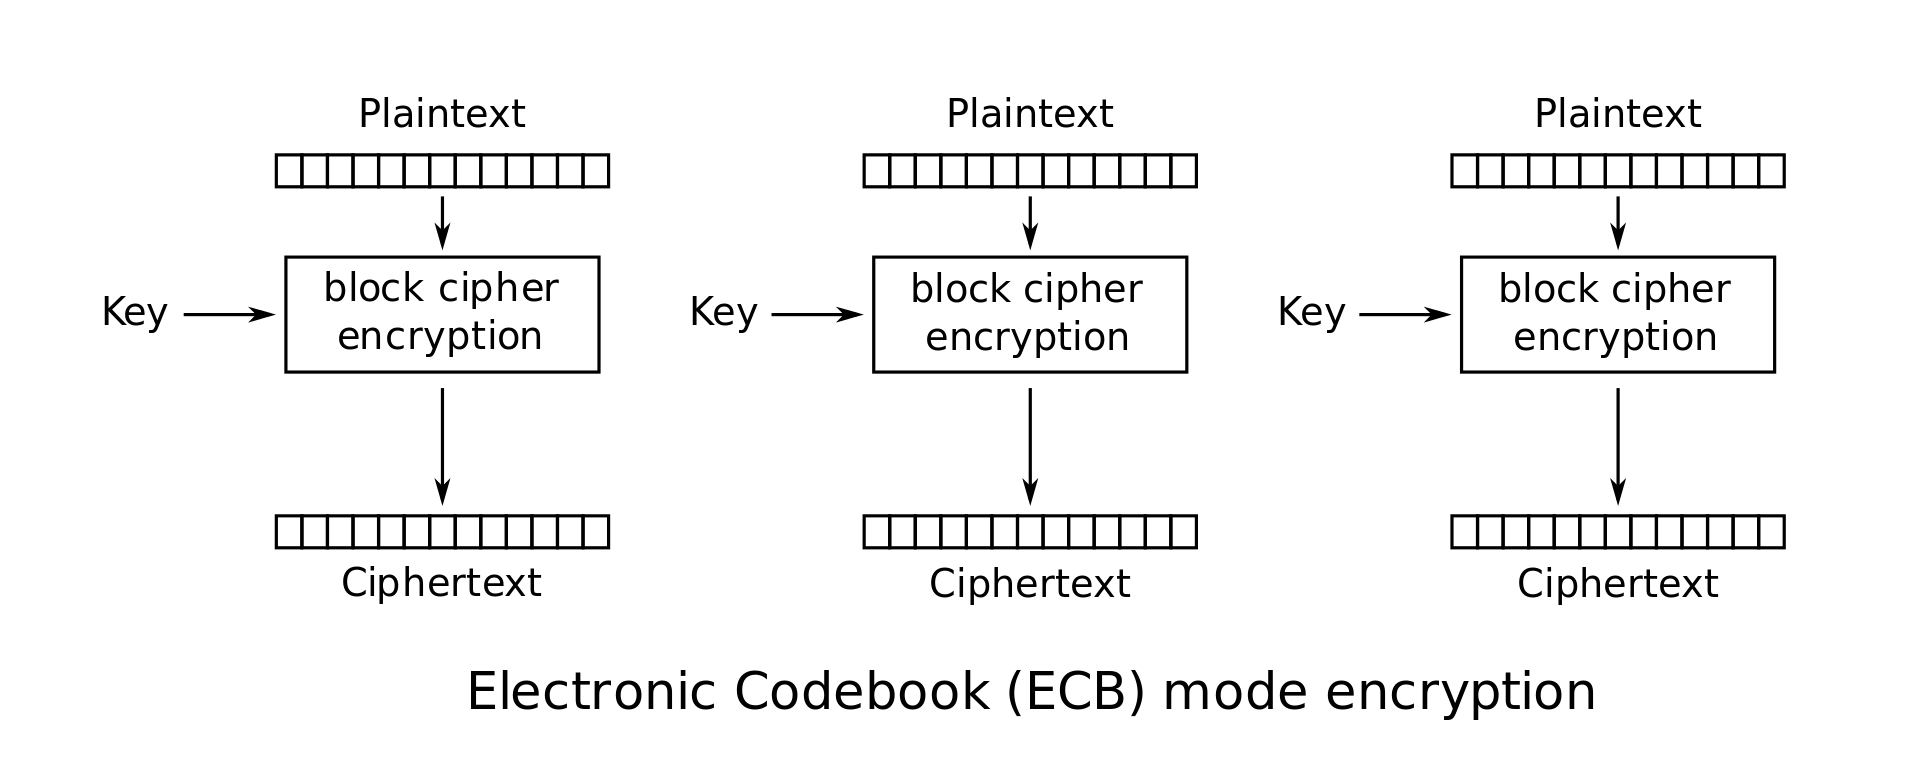
\includegraphics[width=1\linewidth]{kry_1/rezim_ecb.png}
    \caption{Ukázka režimu ECB.}
\end{figure}

\subsection*{Cipher Block Chaining (CBC)}

V~režimu CBC (\uv{řetězení šifrových bloků}) je každý blok před šifrováním xorován zašifrovaným předchozím blokem a první blok je xorován inicializačním vektorem. Tento režim je široce používán. Nevýhody plynou ze zřetězené závislosti (šifrovaný blok závisí na všech předcházejících): Šifrování nelze paralelizovat a při poškození šifrového bloku nelze dešifrovat ani blok přímo následující. Dešifrování paralelizovat lze.

\begin{equation}
\begin{aligned}
C_i &= E_K (P_i \oplus C_{i-1}) \\
P_i &= D_K(C_i) \oplus C_{i-1} \\
C_0 &= IV
\end{aligned}
\end{equation}

\begin{figure}[H]
    \centering
    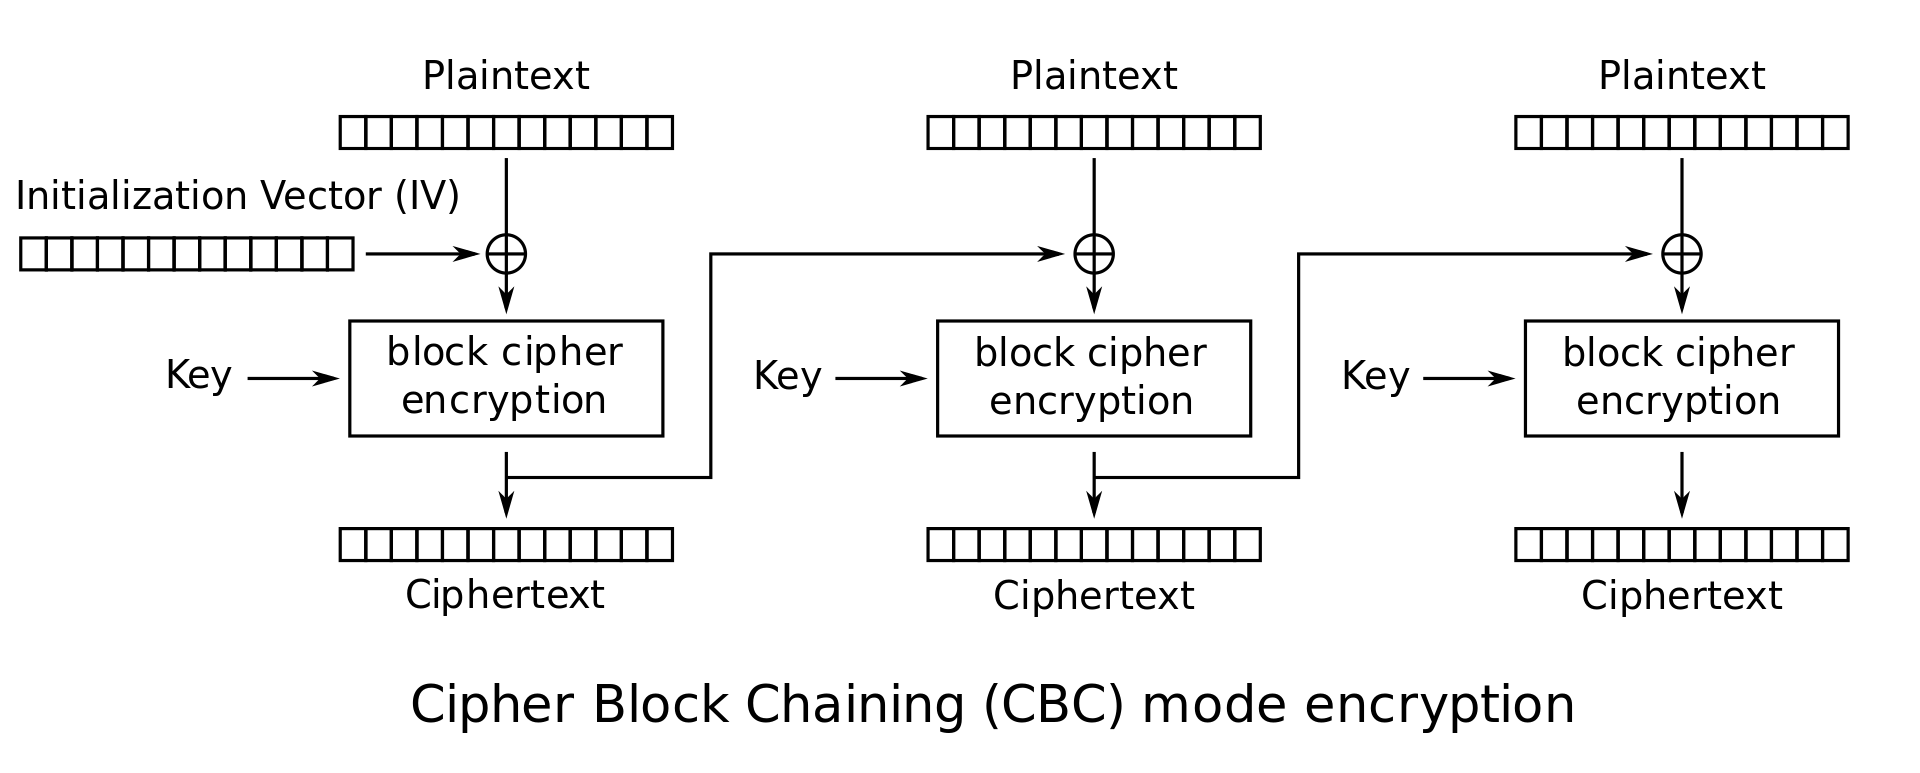
\includegraphics[width=1\linewidth]{kry_1/rezim_cbc.png}
    \caption{Ukázka režimu CBC.}
\end{figure}

\subsection*{Cipher Feedback (CFB)}

Režim CFB (\textit{šifrová zpětná vazba}) se liší oproti CBC v~prohození pořadí operací xor a šifrování -- nejprve se zašifruje předchozí šifrovaný blok (resp. inicializační vektor) a výsledek se xoruje s~otevřeným blokem. Toto prohození má významné implementační dopady: díky symetrii operace XOR vypadá dešifrovací funkce obdobně jako šifrovací. Šifruje pomaleji než CBC. Vstup není nutné zarovnávat. Plynou stejné nevýhody jako pro CBC.

\begin{equation}
\begin{aligned}
C_i &= E_K (C_{i-1}) \oplus P_i \\
P_i &= E_K (C_{i-1}) \oplus C_i \\
C_0 &= IV
\end{aligned}
\end{equation}

\begin{figure}[H]
    \centering
    
\includegraphics[width=1\linewidth]{kry_1/rezim_cfb.png}
    \caption{Ukázka režimu CFB.}
\end{figure}

\subsection*{Output Feedback (OFB)}

Režim OFB (\textit{výstupní zpětná vazba}) se liší od CFB pouze v~tom, kde bere zpětnou vazbu. Šifrování probíhá pouhým xorováním otevřeného bloku s~heslem, které je v~každém kroku zašifrováno použitou blokovou šifrou. První blok hesla je získán zašifrováním inicializačního vektoru. Režim převádí blokovou šifru na synchronní proudovou šifru.

\paragraph*{Slabina} Celý blok encryption je pouze generátor pseudonáhdon posloupnosti (je nezávislá na otevřeném nebo šifrovaném textu). To umožňuje Known Plaintext Attack. Z~toho plyne, že jedním klíčem není bezpečné šifrovat více než jednu zprávu.

\begin{equation}
\begin{aligned}
C_i &= E_K (C_{i-1}) \\
P_i &= P_i \oplus C_i \\
C_0 &= IV
\end{aligned}
\end{equation}

\begin{figure}[H]
    \centering
    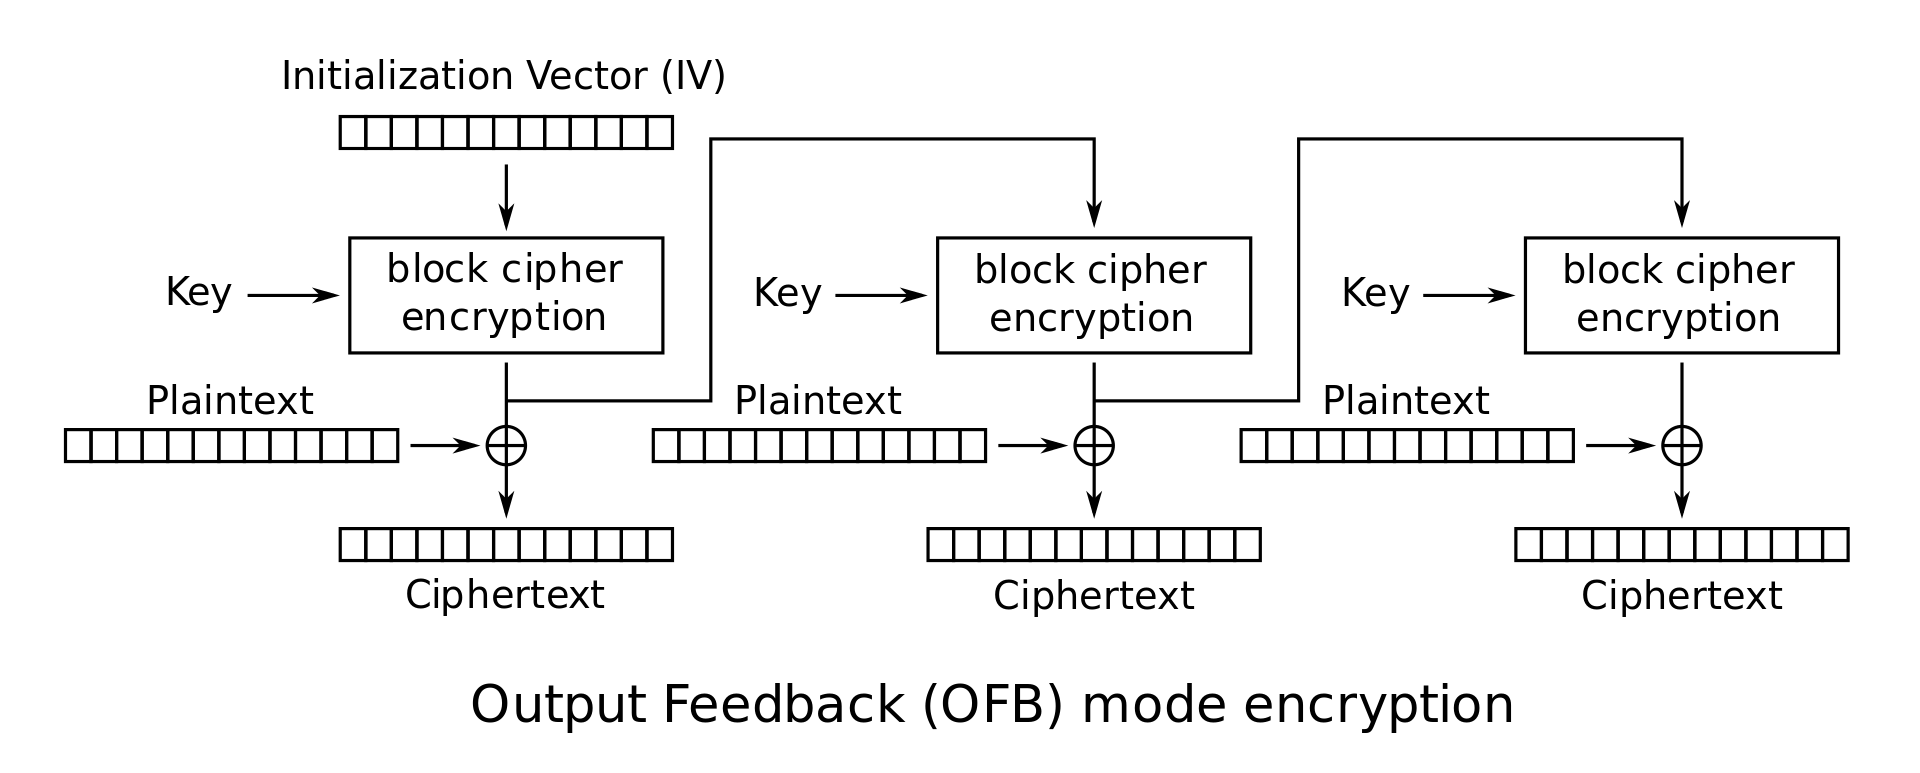
\includegraphics[width=1\linewidth]{kry_1/rezim_ofb.png}
    \caption{Ukázka režimu OFB.}
\end{figure}

\subsection*{Counter (CTR)}

Režim CTR (\uv{čítačový režim}) převádí stejně jako OFB blokovou šifru na synchronní proudovou. Heslo, se kterým se blok otevřeného textu xoruje, je však získáno zašifrováním čítače, který se každou iteraci zvětšuje o~pevně danou hodnotu, zpravidla o~1. Obsah čítače je opět před šifrováním nastaven inicializačním vektorem. Každý blok je šifrován nezávisle na ostatních, díky tomu je možné paralelizovat.

\begin{equation}
\begin{aligned}
CTR_i &= CTR_{i-1} + 1 \\
P_i &= P_i \oplus E_k(CTR_i) \\
CTR_0 &= IV
\end{aligned}
\end{equation}

\begin{figure}[H]
    \centering
    \includegraphics[width=1\linewidth]{kry_1/rezim_ctr.png}
    \caption{Ukázka režimu CTR.}
\end{figure}

%%%%%%%%%%%%%%%%%%%%%%%%%%%%%%%%%%%%%%%%%%%%%%%%%%%%%%%%%%%%%%%%%%%%%%%%%%%%%%%%

\section{Proudové šifry}

Proudové šifry šifrují data jako \textit{proud} (stream), nejčastěji po jednotlivých bytech. Dešifrování vždy probíhá stejným způsobem. Proudové šifry jsou rychlejší než blokové šifry a pro implementaci potřebují jednodušší hardware.

\paragraph*{Problémy} \begin{compactitem}
    \item Nezajišťují samy o~sobě integritu.
    \item Na rozdíl od blokových šifer jsou náchylnější ke kryptoanalytickým útokům, pokud jsou nevhodně implementovány (počáteční stav nesmí být použit opakovaně)~--~\uv{problém s~inicializačním vektorem}.
\end{compactitem}

\begin{figure}[H]
    \centering
    \includegraphics[width=1\linewidth]{kry_1/proudove.png}
    \caption{Princip proudových šifer.}
\end{figure}

\subsection*{Rozdělení proudových šifer}

\paragraph*{Synchronní proudové šifry} Proud pseudonáhodných čísel \textit{key stream} je generován nezávisle na vstupním textu nebo zašifrované zprávě. Poté dochází ke kombinaci vygenerovaných čísel se vstupujícím textem (k~zakódování) nebo se šifrovaným textem (k~dekódování). Nejběžnější formou kombinace keystreamu a vstupního textu je použití operace XOR. Např.: Vernamova šifra, DES v~režimu OFB. Pokud se průběhu dešifrování něco ztratí, je konec.

\begin{figure}[H]
    \centering
    \includegraphics[width=0.5\linewidth]{kry_1/proudova_synchronni.png}
    \caption{Princip synchronní proudové šifry.}
\end{figure}

\paragraph*{Samosynchronizující proudové šifry} Proud pseudonáhodných čísel \textit{key stream} závisí na pevném počtu předcházejících bytů šifrovaného (nebo otevřeného) textu. To znamená, že se šifra dokáže po chybě sama \textit{zotavit} (resynchronizovat)\footnote{Dnes se nesnážíme dešifrovat poškozená data, pokud nastane chyba v~přenosu, vyžádáme si data znovu.}. Např.: Vigenere Autokey, DES v~řežimu CFB.

\begin{figure}[H]
    \centering
    \includegraphics[width=0.75\linewidth]{kry_1/proudova_samosynchronizujici.png}
    \caption{Princip samosynchronizující proudové šifry.}
\end{figure}

\subsection*{Generátory PRNG}

Generátory PRNG (\textit{pseudo-random number generator}) generují pseudo-náhodnou pos\-loupnost (\textit{key stream}) z~malého klíče (\textit{seed}).

\paragraph*{Blokové šifry v~režimu OFB} Blokové šifry v~režimu OFB jsou pomalé.

\paragraph*{Linear Feedback Shift Registers (LSFR)} LFSR (posuvný registr s~lineární zpětnou vazbou) je posuvný registr, jehož výstup je lineárně závislý na jeho předchozích výstupech a stavu. Mějme \begin{compactitem}
    \item posuvný registr $R = (r_1, r_2, \dots, r_n)$,
    \item sekvenci zpětných vazeb $T = (t_1, t_2, \dots, t_n)$.
\end{compactitem}

\noindent Alternativně lze zapsat polynomem: $$
T(x) = x^n + x^{n-1} + \ldots + x + 1
$$

\begin{figure}[H]
    \centering
    \includegraphics[width=0.6\linewidth]{kry_1/lfsr.png}
    \caption{Příklad LFSR.}
\end{figure}

\paragraph*{Geffe generátor} Geffe generátor (kombinovaný generátor) je využití 2 a více LFSR propojených multiplexorem.

\begin{figure}[H]
    \centering
    \includegraphics[width=0.75\linewidth]{kry_1/geffe.png}
    \caption{Příklad Geffe generátoru.}
\end{figure}

\paragraph*{Stop and Go generátor} Stop and Go generátor je několik LSFR s~různým zdrojem hodin.

\begin{figure}[H]
    \centering
    \includegraphics[width=0.8\linewidth]{kry_1/stop_and_go.png}
    \caption{Příklad Stop and Go generátoru.}
\end{figure}

\newpage

% VUT FIT MITAI
% MSZ 2021/2022
% Author: Vladimir Dusek
% Login: xdusek27

%%%%%%%%%%%%%%%%%%%%%%%%%%%%%%%%%%%%%%%%%%%%%%%%%%%%%%%%%%%%%%%%%%%%%%%%%%%%%%%%

\chapter{Asymetrická kryptografie, vlastnosti, způsoby použití, poskytované bezpečnostní funkce, elektronický podpis a jeho vlastnosti, hybridní kryptografie, algoritmus RSA, generování klíčů, šifrování, dešifrování.}

% Todo:
% - Matematicke problemy by sly formulovat lepe a formalneji. To co tu mam, by lehce nemuselo stacit. Kouknout k materialum od Mateje Kastaka.
% Kongruence, multiplikativni inverze

%%%%%%%%%%%%%%%%%%%%%%%%%%%%%%%%%%%%%%%%%%%%%%%%%%%%%%%%%%%%%%%%%%%%%%%%%%%%%%%%

\section{Metadata}

\begin{compactitem}
    \item Předmět: Kryptografie (KRY)
    \item Přednáška:
    \begin{compactitem}
        \item 6) Asymetrická kryptografie, vlastnosti, způsoby použití, poskytované bezpečnostní funkce.
        \item 7) Elektronický podpis a jeho vlastnosti, hybridní kryptografie.
        \item 8) Příklady asymetrických algoritmů, RSA.
    \end{compactitem}
    \item Záznam:
    \begin{compactitem}
        \item 2021-03-08
        \item 2021-03-22
    \end{compactitem}
\end{compactitem}

%%%%%%%%%%%%%%%%%%%%%%%%%%%%%%%%%%%%%%%%%%%%%%%%%%%%%%%%%%%%%%%%%%%%%%%%%%%%%%%%

\section{Úvod a kontext}

\textit{Viz. \uv{Úvod a kontext} v předchozích otázkách z tohoto předmětu.}

\paragraph*{Asymetrická kryptografie} \begin{compactitem}
    \item V asymetrické kryptografii se používají páry klíčů (soukromý a veřejný). Soukromý je používán k dešifrování, resp. vytvoření digitálního podpisu. Veřejný je používán k šifrování, resp. ověření digitálního podpisu.
    \item Každý uživatel generuje svůj pár klíčů. Veřejný klíč je zveřejněn (znají ho všichni), sourkomý je držen v tajnosti (zná ho pouze vlastník).
    \item Všechny asymetrické algoritmy jsou blokové.
    \item Asymetrické algoritmy jsou pomalejší než symetrické.
\end{compactitem}

\paragraph*{Způsoby použití} Asymetrická kryptografie lze využít k: \begin{compactitem}
    \item šifrování,
    \item digitálnímu podepisování,
    \item pro výměnu symetrického klíče (\textit{key exchange}).
\end{compactitem}

\paragraph*{Vlastnosti} Vlastnosti symetrické a asymetrické kryptografie\footnote{Otazníky -- částečně, za předpokladů, \dots}.
\begin{table}[H]
\begin{tabular}{lllll}
& Důvěrnost & Autentizace & Integrita & Nepopiratelnost \\
Symetrická & ano & ? & ? & ne \\
Asymetrická - šifrování & ano & ? & ? & ne \\
Asymetrická - podepisování & ne & ano & ano & ano \\
Asymetrická - kombinace & ano & ano & ano & ano
\end{tabular}
\end{table}

\bigskip\noindent\begin{minipage}{\linewidth}
\begin{lstlisting}[language=Python, caption={Kombinace klíčů obou stran u asymetrický kryptografie. Pořadí operací může být i opačné.}]
# Odesilatel (A):
msg = encrypt(msg, SK_A) # necht msg je zprava k odeslani
msg = encrypt(msg, PK_B)
send(msg_2)

# Prijemce (B):
msg = receive()
msg = decrypt(msg, SK_B)
msg = decrypt(msg, PK_A)
\end{lstlisting}
\end{minipage}

\paragraph*{Digitální podpis} Vytvoření digitálního podpisu konkrétních dat pomocí soukromého klíče podepisatele. Každý kdo zná veřejný klíč podepisatele, může pravost podpisu ověřit. Digitální podpis zajišťuje autentizaci, itegritu a nepopiratelnost.

\paragraph*{Algoritmy} Algoritmy asymetrické kryptografie se nedají \textit{vymyslet}, musí se objevit. Jsou založeny na těžkých matematických problémech. \begin{compactitem}
    \item Problém batohu (\textit{knapsack problem}) -- MH (Merkle-Hellman)
    \item Faktorizace čísel -- RSA (Rivest-Shamir-Adleman)
    \item Diskrétní logaritmus -- DSA (Digital Signature Algorithm), DH (Diffie-Hellman)
    \item Eliptické křivky -- ECDSA, ECDH
\end{compactitem}

\paragraph*{Problém batohu} Problém batohu je NP-úplný problém kombinatorické optimalizace. Nechť ${x_1, x_2, \dots, x_n}$ je množina objektů, každý objekt má svoji cenu $v_i$ a svoji hmotnost $w_i$, dále mějme batoh, který má kapacitu $W$. Cílem je vybrat takovou množinu objektů, jejichž hmotnost je menší nebo rovna $W$ a má nejvyšší možnou cenu\footnote{Problém má více obdobných variant.}. Formálně chceme maximalizovat sumu $$ \sum_{i=1}^n v_i \cdot x_i $$, při splnění $$ \sum_{i=1}^n w_i \cdot x_i \leq W $$, kde $x_i \in {x_1, x_2, \dots, x_n}$.

\paragraph*{Faktorizace čísel} Faktorizace čísel označuje problém rozložení čísla na součin menších čísel, v nejčastější podobě pak rozklad celého čísla na součin prvočísel.

\paragraph*{Diskrétní logaritmus} Nechť $p, g, k, Y$ jsou přirozená čísla, pro něž platí $Y \equiv g^{k} \; \text{mod} \; p$. Potom každé číslo $k$ odpovídající uvedené rovnici nazveme diskrétní logaritmus o základu $g$ z $Y$ vzhledem k modulu $p$. Tato definice nedefinuje číslo $k$ jednoznačně, proto se někdy upravuje tak, že ze všech možných diskrétních logaritmů ve smyslu předchozí definice se vybere ten nejmenší.

\paragraph*{Eliptické křivky} Jedná se o matematický aparát, na kterém aplikujeme různé algoritmy (DSA, DH).

%%%%%%%%%%%%%%%%%%%%%%%%%%%%%%%%%%%%%%%%%%%%%%%%%%%%%%%%%%%%%%%%%%%%%%%%%%%%%%%%

\section{Hybridní kryptografie}

Hybridní kryptografie je kombinace symetrické a asymetrické kryptografie, ve které jsou využity přednosti obou (symetrická -- rychlá, ale potřeba stejný klíč; asymetrická -- pomalá, ale dva klíče). Asymetrická je využita pro bezpečné zaslání symetrického klíče.

\begin{figure}[H]
    \centering
    \includegraphics[width=1\linewidth]{kry_2/hybrid_utajeni.pdf}
    \caption{Schéma utajení hybridní kryptografie.}
\end{figure}

\begin{figure}[H]
    \centering
    \includegraphics[width=1\linewidth]{kry_2/hybrid_podpis.pdf}
    \caption{Schéma digitálního podpisu hybridní kryptografie.}
\end{figure}

%%%%%%%%%%%%%%%%%%%%%%%%%%%%%%%%%%%%%%%%%%%%%%%%%%%%%%%%%%%%%%%%%%%%%%%%%%%%%%%%

\section{RSA}

Algoritmus RSA (Rivest-Shamir-Adleman) lze použít jak pro šifrování dat pro digitální podepisování. Je založen na problému faktorizace velkých čísel.

\paragraph*{Klíče} Klíče se skládají z: \begin{compactitem}
    \item $p, q$ -- dvě náhodná soukromá prvočísla,
    \item $n$ -- veřejný modul ($n = p \cdot q$),
    \item $e$ -- veřejný exponent ($e < \Phi(n) \; \land \; GCD(\Phi(n), e) = 1$), typicky $3$ nebo $2^{16}+1$\footnote{$GCD$~--~největší společný dělitel},
    \item $d$ -- soukromý exponent,
    \item musí platit vztah: $e \cdot d \; \text{mod} \; \Phi(n) = 1$.
\end{compactitem}

\noindent Veřejný klíč $PK = (n, e)$, soukromý klíč $SK = (n, d)$.

\paragraph*{Postup generování} Postup generování klíčů: \begin{compactenum}
    \item vygenerovat prvočísla $p$ a $q$,
    \item spočítat modul $n = p \cdot q$,
    \item spočítat $\Phi(n) = (p-1) \cdot (q-1)$,
    \item zvolit veřejný exponent $e < \Phi(n) \; \land \;GCD(\Phi(n), e) = 1$,
    \item spočítat soukromý exponent $d$ tak, že platí $e \cdot d \; \text{mod} \; \Phi(n) = 1$.
\end{compactenum}

\paragraph*{Šifrování a dešifrování} Mějme zprávu $m$ reprezentovanou jako celé číslo a zašifrovanou zprávu $c$ reprezentovanou také jako celé číslo. Digitální podpis se vytváří stejným způsobem, pouze se prohodí exponenty.

\begin{equation}
    c = m^e \; \text{mod} \; n
\end{equation}

\begin{equation}
    m = c^d \; \text{mod} \; n
\end{equation}

\paragraph*{Útoky a slabiny} Pokud útočník rozloží číslo $n$ na činitele $p$ a $q$, tak může dopočítat soukromý klíč. Pokud útočník uhádně hodnotu $(p-1) \cdot (q-1)$, tak může dopočítat soukromý klíč. Šifrování malých čísel je zranitelné, proto se používá \uv{předzpracování}~--~zarovnání na $X$ bitů (2048).

\begin{figure}[H]
    \centering
    \includegraphics[width=1\linewidth]{kry_2/rsa_example.pdf}
    \caption{Příklad RSA.}
\end{figure}

\newpage

% VUT FIT MITAI
% MSZ 2021/2022
% Author: Vladimir Dusek
% Login: xdusek27

%%%%%%%%%%%%%%%%%%%%%%%%%%%%%%%%%%%%%%%%%%%%%%%%%%%%%%%%%%%%%%%%%%%%%%%%%%%%%%%%

\chapter{Hašovací funkce, klíčovaný haš a MAC a jejich použití a vlastnosti.}

%%%%%%%%%%%%%%%%%%%%%%%%%%%%%%%%%%%%%%%%%%%%%%%%%%%%%%%%%%%%%%%%%%%%%%%%%%%%%%%%

\section{Metadata}

\begin{compactitem}
    \item Předmět: Kryptografie (KRY)
    \item Přednáška:
    \begin{compactitem}
        \item \path{KRY04_Asym_MNG.pdf}
    \end{compactitem}
    \item Záznam:
    \begin{compactitem}
        \item 2021-03-22
    \end{compactitem}
\end{compactitem}

%%%%%%%%%%%%%%%%%%%%%%%%%%%%%%%%%%%%%%%%%%%%%%%%%%%%%%%%%%%%%%%%%%%%%%%%%%%%%%%%

\section{Historie položení otázky}

\begin{compactitem}
    \item Rok: 2013
    \item Jméno otázky: Haš, klíčovaný haš, HMAC
    \item Zkoušel: Hanáček Petr, doc. Dr. Ing.
    \item Známka: E
    \item Zacal jsem definici hasovaci funkce, ten slajd, pak padla otázka klíčovaný has, tak zas definice co to je a tak. Potom chtěl vědět útoky a složitost útoku a jeho pravděpodobnost. K tomu jsme se s jeho značnou pomocí úspěšně dobrali. Dost pomáhal.
\end{compactitem}

\begin{compactitem}
    \item Rok: 2014
    \item Jméno otázky: Hašovací funkce, klíčovaný haš a MAC a jejich použití a vlastnosti
    \item Zkoušel: Hanáček Petr, doc. Dr. Ing.
    \item Známka: E
    \item Co jsem k tomu rekl(a)/na co se ptali/co mne vytkli: Ptal se na MAC, říkal jsem že slouží pro podpis a začal jmenovat ty 3 potřebné podmínky pro hash.funkce. Tím sem si sám naběhl, protože jsem zapomněl 2nd preimage. Na to, co jsem místo toho "vyvařil", řekl, že to je ale 1st preimage, a chtěl to vědět správně, nakonec to musel říct za mě. Dál se ptal na sílu hashe, takové to, co bylo i letos na zkoušce, že pro útok vůči collision resistance je složitost $2^{80}$ i když hash má délku $2^{160}$. Patlal jsem se v tom, tak nakonec chtěl přesně vědět jak se na každou věc útočí a jakou složitost to bude mít.
\end{compactitem}

\begin{compactitem}
    \item Rok: 2015
    \item Jméno otázky: Hašovací funkce, klíčovaný haš, MAC
    \item Zkoušel: Hanáček Petr, doc. Dr. Ing.
    \item Známka: E
    \item Začal jsem tím, co je to hašovací funkce, jaké jsou na ní kladené podmínky (preimage resistance, ...). Tam mě Hanáček přerušil a začal se ptát, kolik pokusů musí útočník vyzkoušet při útoku hrubou silou, aby pokořil každou z těch podmínek. Úplně jsem se do toho zamotal, rozklepal jsem se a nebyl schopen kloudného slova. Hanáčkův poker face v tom taky nijak nepomáhal, ale asi se snažil nějak pomoct (To n značí prostor vstupních dat? Jak chcete, jen se ptám.), a ačkoli jsem to věděl, nebyl jsem v tu chvíli schopen formulovat odpověď. Nechal mě v tom ještě hodnou chvíli koupat a pak to ukončil.
\end{compactitem}

\begin{compactitem}
    \item Rok: 2018
    \item Jméno otázky: Hašovací funkce, klíčovaný haš a MAC a jejich použití a vlastnosti
    \item Zkoušel: Hanáček Petr, doc. Dr. Ing.
    \item Známka: B
    \item Prvně jsem uvedl co je hašovací funkce (základní definice, first preimage resistance, second preimage resistance, collision resistance). P. Hanáček se následně začal doptávat na vztah mezi second preimage resistance a collision resistance včetně potřebné síly útoku. Kolem tohoto tématu jsme se točili asi další 2 minuty. Následně se P. Hanáček dotázal na klíčovaný haš a MAC, což jsem obecně popsal. Zmínil jsem také jakým způsobem se klíč přidává ke zprávě a částečně jsem popsal HMAC. Následně se P. Hanáček zeptal, k čemu je klíčovaný haš dobrý - uvedl jsem, že zajišťuje integritu dat a autentizaci, což se při neklíčovaných hašovacích funkcí musí zajistit například podpisem pomocí asymetrické šifry. Tím také zkoušení skončilo. Trvalo 5-6 minut. Přestože, jsem byl na tuto otázku připraven, nebylo zkoušení moc příjemné a P. Hanáček mě občas dokázal docela znejistit.
\end{compactitem}

\begin{compactitem}
    \item Rok: 2018
    \item Jméno otázky: Hašovací funkce, klíčovaný haš a MAC a jejich použití a vlastnosti
    \item Zkoušel: Hanáček Petr, doc. Dr. Ing.
    \item Známka: A
    \item Začal jsem takové obecné kecy a rychle se přesunul na požadavky/vlastnosti, které chceme aby hashovací funkce měla. Popsal jsem First Preimage, Second Preimage a Collision Resistance. Pak jsme docela dlouho zůstali viset na rozdílu mezi second preimage a collision resistance. Celkově se mi pan docent snažil naznačit, jak mám mezi nimi tedy určit ten rozdíl. Ptal se mne pak jak je to s útoky, tak jsem zmínil, že je zde Birthday paradox, a uvedl jsem, že na 160 bitech stačí typicky projít $2^{80}$ možností než dojdu ke kolizi. Na to myslím, námitky nebyly a přesunuli jsme se ke klíčovanému haši. Někde na začátku zazvonil budík, ale jeli jsme dál. Řekl jsem, že tam je ten klíč, a řekl jsem, že jsme si uvedli některé typy použití, ale nejvýznamnější je HMAC. Zeptal jsem se, zda jej chce popsat, což nechtěl. Načež byl dotaz -- K čemu ten klíčovaný hash slouží, tak jsem řekl že autentizaci. S tím pan docent souhlasil. Zeptal se mne, že co to znamená pro útočníka z hlediska bezpečnosti, tak jsem řekl, že je to pro něj horší, protože nezná klíč, což sice částečně potvrdil, ale chtěl pak ještě něco, ale to už si napamatuji a nevěděl jsem to.
\end{compactitem}

%%%%%%%%%%%%%%%%%%%%%%%%%%%%%%%%%%%%%%%%%%%%%%%%%%%%%%%%%%%%%%%%%%%%%%%%%%%%%%%%

\section{Úvod a kontext}

\textit{Viz. \uv{Úvod a kontext} v~předchozích otázkách z~tohoto předmětu.}

\paragraph*{Hashovací funkce} Hashovací funkce je funkce (resp. algoritmus) pro převod vstupních dat do (relativně) malého čísla. Výstup hashovací funkce se označuje otisk, \textit{fingerprint}, \textit{digest} či \textit{hash}. Jsou jednosměrné a odolné proti kolizím (viz vlastnosti).

\paragraph*{Obecné vlastnosti} Hashovací funkce by měla: \begin{compactitem}
    \item Být aplikovatelná na argument o~libovolné velikosti.
    \item Mít výstyp konstantní délky.
    \item Dokázat spočítat výstup rychle.
\end{compactitem}

\paragraph*{Neklíčované hashovací funkce} Hashovací funkce má pouze jeden argument~--~data. Např. MD2, MD4, MD5, SHS, SHA1, SHA2, SHA3. $$f(data) \rightarrow hash$$

\paragraph*{Klíčované hashovací funkce} Hashovací funkce má dva argumenty~--~data a klíč. Také se jim někdy říká MAC (\textit{message authentication code}). $$f(data, key) \rightarrow hash$$

%%%%%%%%%%%%%%%%%%%%%%%%%%%%%%%%%%%%%%%%%%%%%%%%%%%%%%%%%%%%%%%%%%%%%%%%%%%%%%%%

\section{Kryptografická odolnost hashovacích funkcí}

\paragraph*{Vlastnosti z~hlediska odolnosti} Hashovací funkce by z~hlediska kryptografické odolnosti měly splňovat: \begin{compactitem}
    \item \textit{First preimage resistance}~--~Pro konkrétní $y$ je výpočetně nezvládnutelné najít takové $x$, aby platilo $h(x) = y$. Útočník má k~dispozici konkrétní hash, a snaží se pro něho nalézt zprávu.
    \item \textit{Second preimage resistance}~--~Pro konkrétní $x$ je výpočetně nezvládnutelné najít takové $x'$, aby platilo $h(x) = h(x')$. Útočník má k~dispozici konkrétní zprávu (nemůže si ji zvolit), ke které se snaží nalézt jinou zprávu, která bude mít stejný hash.
    \item \textit{Collision resistance}~--~Je výpočetně nezvládnutelné najít libovolnou dvojici $x, x'$ takovou, aby platilo $x \neq x'$ a $h(x) = h(x')$. Útočník si může zvolit libovolnou zprávu, ke které se snaží nalézt jinou zprávu, která bude mít stejný hash. Pokud platí \textit{collision resistance}, tak platí i \textit{second preimage resistance}.
\end{compactitem}

\paragraph*{Narozeninový problém} V~teorii pravděpodobnosti je narozeninový problém úloha vypočítat minimální početnost skupiny lidí, ve které je alespoň 50\% pravděpodobnost nalezení dvojice se stejným datem narození. Narozeninovým paradoxem je pak označována skutečnost, že tento počet (23) je mnohem menší než intuitivní odhad.
Výsledek je intuitivnější, když uvážíme, že porovnání narozenin bude provedeno mezi všemi možnými dvojicemi jedinců. Při počtu 23 jedinců je třeba uvažovat $(23 \cdot 22) / 2 = 253$ dvojic, což je více než polovina počtu dnů v~roce ($182,5$).

Jednodušší je nejprve spočítat jev opačný $\bar p(n)$, tedy pravděpodobnost, že všech $n$ narozenin je rozdílných. Pro $n > 365$ je $1$, jinak:
\begin{equation}
\begin{aligned}
\bar p(n) &= 1 \cdot \left(1-\frac{1}{365}\right) \cdot \left(1-\frac{2}{365}\right) \cdots \left(1-\frac{n-1}{365}\right) = \\
&=  \frac{365 \cdot 364 \cdots (365-n+1)}{365^n} = \\
&=  \frac{365!}{365^n (365-n)!}
\end{aligned}
\end{equation}

\begin{equation}
    p(n) = 1 - \bar p(n)
\end{equation}

\paragraph*{Narozeninový útok} Mějme hashovací funkci, která má $n$ bitový výstup (celkový počet možných hashů je $2^{n}$). Útočník vytvoří dokument \uv{přátelská dohoda} a přibližně $2^{n/2}$ sémanticky ekvivalentních verzí (úprava bílých znaků, úprava pořadí celků, jiné formulace, \dots). Podobně vytvoří dokument \uv{nepřátelská dohoda} a přibližně $2^{n/2}$ sémanticky ekvivalentních verzí. S~pravděpodobností $0,5$ existuje verze \uv{přátelské dohody} a \uv{nepřátelské dohody}, které mají stejný hash. Pokud takové verze existují, útočník dá oběti podepsat \uv{přátelskou dohodu} $\Rightarrow$ existuje validní podpis \uv{nepřátelské dohody}.

\paragraph*{Bezpečnostní cíle OWHF} Bezpečnostní cíle OWHF (\textit{one way hash function}). Některé protokoly nevyžadují bezkoliznost, proto má smysl řešit i tento případ. \begin{compactitem}
    \item Vyžadované vlastnosti: \textit{first preimage resistance} a \textit{second preimage resistance}
    \item Cíl útočníka: vytvořit \textit{first preimage} nebo \textit{second preimage} (oba úkoly jsou stejně těžké)
    \item Složitost: $O(2^n)$ ($n$ je počet bitů hashe)
    \item Požadovaná délka: $n \geq 80$
\end{compactitem}

\paragraph*{Bezpečnostní cíle CRHF} Bezpečnostní cíle CRHF (\textit{collision resistance hash function}). \begin{compactitem}
    \item Vyžadované vlastnosti: \textit{collision resistance}
    \item Cíl útočníka: vytvořit kolizi
    \item Složitost: $O(2^{n / 2})$ ($n$ je počet bitů hashe) (kvůli narozeninovému útoku)
    \item Požadovaná délka: $n \geq 160$
\end{compactitem}

\paragraph*{Bezpečnostní cíle MAC} Bezpečnostní cíle MAC (\textit{message authentication code}). \begin{compactitem}
    \item Vyžadované vlastnosti: \textit{computation resistance}, \textit{key non-recovery}
    \item Cíl útočníka (útočník si může vybrat): \begin{compactitem}
        \item Vytvořit nový hash, který bude odpovídat nové zprávě
        \item Nalézt klíč
    \end{compactitem}
    \item Složitost ($n$ je počet bitů hashe, $t$ je počet bitů klíče): \begin{compactitem}
        \item Vytvořit nový hash: $O(max(2^{-n}, 2^{-t}))$
        \item Nalézt klíč: $O(2^n)$
    \end{compactitem}
    \item Požadovaná délka: $n \geq 64 \; \land \; t \geq 64$
\end{compactitem}

%%%%%%%%%%%%%%%%%%%%%%%%%%%%%%%%%%%%%%%%%%%%%%%%%%%%%%%%%%%%%%%%%%%%%%%%%%%%%%%%

\section{Hashovací funkce neklíčované}

Nejčastější způsoby sestrojení hashovací funkce neklíčované jsou založené na principu iterace.

\begin{figure}[H]
    \centering
    \includegraphics[width=0.6\linewidth]{kry_3/hash_function_iterative.pdf}
    \caption{Schéma iterativní neklíčované hashovací funkce. Zpráva je rozdělena na $n$ částí. $f$ je tzv. kompresní funkce. $IV$ je inicializační vektor, resp. konstanta. $h_1$ až $h_{n-1}$ jsou mezivýsledky (\uv{mezihashe}) a $h$ je výsledný hash.}
\end{figure}

\begin{figure}[H]
    \centering
    \includegraphics[width=0.9\linewidth]{kry_3/hash_function_iterative_detail.pdf}
    \caption{Podrobnější schéma iterativní neklíčované hashovací funkce.}
\end{figure}

Jednotlivé kroky hashovací funkce: \begin{compactitem}
    \item Předzpracování~--~Vstupní data jsou rozdělena na bloky o~stejné délce. Je provedeno zarovnání posledního bloku. Je připojena informace o~délce zprávy.
    \item Iterativní zpracování~--~V~iteracích se postupně \uv{přihashovávají} vstupní bloky. Zpět\-ná vazba pomocí stavové proměnné. Uvnitř kompresní funkce, která z~delšího vstupu uděla kratší výstup.
    \item Postzpracování~--~Volitelný krok.
\end{compactitem}

\paragraph*{Merkelova meta-metoda} Nechť $f$ je kompresní funkce odolná proti kolizím. Hashovací funkce $h$ na principu iterace využívající kompresní funkci $f$ je rovněž odolná proti kolizím.

\paragraph*{Merkel-Damgardovo zesílení} Pokud je do vstupu hashovací funkce vložena délka zprá\-vy, tak je zajištěno, že žádná zpráva není prefixem jiné zprávy.

\paragraph*{Zarovnání} Nejednoznačné zarovnání (\textit{ambiguous padding}) -- připoj ke zprávě tolik bitů, aby délka zprávy byla násobkem délky bloku. Jednoznačné zarovnání (\textit{unambiguous padding}) -- připoj ke zprávě jeden bit a poté proveď nejednoznačné zarovnání.

\subsection*{Hashovací funkce s~využitím blokových šifer}

Alternativně lze využít pro konstrukci hashovacích funkcí blokové šifry. Avšak blokové šifry byly navrhovány pro jiný režim činnosti, kterém útočník nezná klíč (a není schopen ho ovlivnit), zná pouze šifrovaný text (ten je schopen ovlivnit). V~tomto případě útočník může přimo ovlivňovat hodnoty klíče.

\begin{figure}[H]
    \centering
    \includegraphics[width=0.9\linewidth]{kry_3/hash_function_blocks.pdf}
    \caption{Ukázka několika možných způsobů využití blokových šifer pro konstrukci kompresní funkce. S~využitím iteračního způsobu lze zobecnit pro celou hashovací funkci.}
\end{figure}

%%%%%%%%%%%%%%%%%%%%%%%%%%%%%%%%%%%%%%%%%%%%%%%%%%%%%%%%%%%%%%%%%%%%%%%%%%%%%%%%

\section{MAC (\textit{message authentication code})}

\begin{compactitem}
    \item Rodina hashovacích funkcí $h_k$, které jsou parametrizovatelné klíčem $k$.
    \item Vlasnosti (stejné jako u~obecných hashovacích funkcí, pouze rozšířené o~klíč): \begin{compactitem}
        \item Výstup $h_k(x)$ lze spočítat rychle, pokud je znám klíč $k$.
        \item Jsou výpočetně bezpečné -- při znalosti dvojice $(x, h_k(x))$ je výpočetně nemožné spočíst novou dvojici $(x', h_k(x'))$, pro $x \neq x'$, pokud není znám klíč.
    \end{compactitem}
    \item Využití: zajištění autentizace a integrity (nepopiratelnost zajistit nedokáže).
\end{compactitem}

\begin{figure}[H]
    \centering
    \includegraphics[width=1\linewidth]{kry_3/mac.png}
    \caption{Schéma použití MAC. Pokud je stejný MAC výpočítán na straně příjemce, tak má jistotu, že zpráva nebyla po cestě změněna a že zprávu poslal skutečně odesílatel.}
\end{figure}

\subsection*{Sestrojení MAC pomocí blokové šifry v~CBC}

Pro sestrojení MAC hashovací funkce je využita symetrická bloková šifra v~režimu CBC (\textit{cipher block chaining}, šifrová zpětná vazba). Rozdíl oproti CBC šifrování spočívá v~tom, že mezivýsledky se zahazují a pracuje se až s~posledním blokem. Z~něho se vezme určitý počet posledních bitů (podle požadované délky hashe -- 32, 48, 64) a ten tvoří výsledný hash (MAC).

\begin{figure}[H]
    \centering
    \includegraphics[width=0.8\linewidth]{kry_3/mac_cbc.png}
    \caption{Ukázka sestrojení MAC funkce pomocí symetrické blokové šifry v~režimu CBC.}
\end{figure}

Proč stačí výrazně menší délka? Protože klíč. Útočník sice může vyzkoušet všechny možné hashe, ale bez znalostí klíče, nezjistí, který je ten správný.

\subsection*{Sestrojení MAC pomocí neklíčované hashovací funkce}

Pro sestrojení MAC hashovací funkce je využita neklíčovaná hashovací funkce. Klíč je připojen ke zprávě a je použita standardní hashovací funkce.

\paragraph*{Secret prefix} Klíč je přidán na začátek zprávy. Formálně: $H = h(k || x)$, kde $H$ je výsledný hash (MAC), $h$ je hashovací funkce, $k$ je klíč a $x$ je zpráva. Útočník může libovolně \uv{přihashovávat} další bloky bez znalosti klíče a tím vytvářet nové validní hashe~--~$h(k || x || y)$, kde $y$ je útočníkova zpráva $\Rightarrow$ nepřijatelný způsob.

\paragraph*{Secret suffix} Klíč je přidán na konec zprávy. Formálně: $H = h(x || k)$. Útočník, který může zvolit $x$, může také vytvořit $x'$, pro které $h(x) = h(x')$ se složitostí $O(2^{n/2})$, kde $n$ je délka hashe, bez ohledu na délku klíče $k$ (narozeninový útok) $\Rightarrow$ nepřijatelný způsob (útok který je neovlivnitelný délkou klíče).

\paragraph*{Enveloping} Klíč je přidán na začátek i na konec zprávy. Formálně: $H = h(k || p || x || k)$, kde $p$ je zarovnání. Přijatelný způsob. Základ pro algoritmus HMAC.

\subsection{HMAC (\textit{hash function MAC})}

HMAC (\textit{hash function MAC}) je do dnes používaný algoritmus. Specifikuje použití metody \textit{enveloping}, ale ne, která hashovací funkce se použije.

\begin{figure}[H]
    \centering
    \includegraphics[width=0.9\linewidth]{kry_3/hmac.png}
    \caption{Schéma HMAC; \texttt{ipad} a \texttt{opad} jsou vstupní/výstupní konstanty, které slouží k~zarovnání; $Y_i$ jsou bloky vstupní zprávy; $IV$ je inicializační vektor.}
\end{figure}

\newpage

% VUT FIT MITAI
% MSZ 2021/2022
% Author: Vladimir Dusek
% Login: xdusek27

%%%%%%%%%%%%%%%%%%%%%%%%%%%%%%%%%%%%%%%%%%%%%%%%%%%%%%%%%%%%%%%%%%%%%%%%%%%%%%%%

\chapter{Správa klíčů v~asymetrické kryptografii (certifikáty X.509).}

%%%%%%%%%%%%%%%%%%%%%%%%%%%%%%%%%%%%%%%%%%%%%%%%%%%%%%%%%%%%%%%%%%%%%%%%%%%%%%%%

\section{Metadata}

\begin{compactitem}
    \item Předmět: Kryptografie (KRY)
    \item Přednáška:
    \begin{compactitem}
        \item \path{KRY04_Asym_MNG.pdf}
    \end{compactitem}
    \item Záznam:
    \begin{compactitem}
        \item 2021-03-29
    \end{compactitem}
\end{compactitem}

%%%%%%%%%%%%%%%%%%%%%%%%%%%%%%%%%%%%%%%%%%%%%%%%%%%%%%%%%%%%%%%%%%%%%%%%%%%%%%%%

\section{Historie položení otázky}

\begin{compactitem}
    \item Rok: 2016
    \item Jméno otázky: Správa klíčů v asymetrické kryptografii
    \item Zkoušel: Staudek Jan, Doc. Ing. CSc.
    \item Známka: E
    \item Předpokládal jsem že se mě ptá Hanáček, začal jsem mluvit směrem k němu, začal jsem o principech asymetrické kryptografie, asi po půl minutě mě přerušil Staudek (který do té doby spal), že tohle vědět nechce, tak jsem začal o certifikátech, zase mě přerušil, že to taky nechce, takhle se to opakovalo ještě jednou, tak jsem se ho přímo zeptal, že co jako chce slyšet, vytřeštil oči a koukal na mě tak se do toho vložil Hanáček, asi se mi snažil nějak pomoct, ale v jeho případě to nepadalo moc na úrodnou půdu, moc jsme si nerozuměli co se týkalo záměn slov certifikát a klíč, motali jsme se v tom, základní myšlenku jsem sice řekl, ale Staudek do toho pořád rýpal, že to slyšet nechce, ale prostě nebylo vůbec jasné, co chce. Byl dost nepřijemný, strašně mumlal, nebylo mu rozumět a když jsem mu nerozuměl a chtěl ať zopakuje otázku, tak odpovídal dost nasraně, jako by to bral jako útok na sebe. Čas jsem překročil asi dvojnásobně, a byť jsem většinu času mluvil, a myslím si že k věci a korektně, tak při odchodu jsem si nebyl úplně jistý, že mi to dá, ale prošlo to.
\end{compactitem}

\begin{compactitem}
    \item Rok: 2018
    \item Jméno otázky: Správa klíčů v asymetrické kryptografii
    \item Zkoušel: doc. Ing. Václav Zeman Ph.D.
    \item Známka: C
    \item Nechal mě chvíli mluvit, řekl jsem že v asym. Jsou 2 klíče - SK, VK, které generuje uživatel, je tam CA, které spravuje a podepisuje VK uživatelů, jaké tam jsou položky. A pak se začal ptát, protože viděl, že vzpomínám tak nějak marně :D. Ptal se na něco ve stylu, jak bych ověřil platnost certifikátu nějakého uživatele, tak jsem začal plácat o tom, že normálně dotaz a pak nad CA je strom CA a ty potvrzují CA… ale chtěl slyšet něco jiného…a poslední otázka byla jak bych to implementoval, že je tam nějaké políčko, na kterém to CA podepisuje tak chtěl vědět jak se jmenuje, to jsem si nevzpomněl, tak řekl, že mu to stačí. Venku mi kamarád řekl, že by se na to dalo použít LDAP... kdo ví.
\end{compactitem}

%%%%%%%%%%%%%%%%%%%%%%%%%%%%%%%%%%%%%%%%%%%%%%%%%%%%%%%%%%%%%%%%%%%%%%%%%%%%%%%%

\section{Úvod a kontext}

\textit{Viz. \uv{Úvod a kontext} v~předchozích otázkách z~tohoto předmětu.}

\paragraph*{Problém se zveřejňováním veřejných klíčů} Jak můžu vědět, že publikovaný veřejný klíč patří opravdu entitě, které patřit má? Je potřeba zajistit autenticitu (pravost) veřejných klíčů~--~Vytvořit spolehlivou vazbu mezi veřejným klíčem a jménem jeho vlastníka.

\paragraph*{Systémy založené na veřejném klíči} Systémy založené na veřejném klíči (PKI, \textit{Public Key Infrastructure}) je označení infrastruktury správy a distribuce veřejných klíčů. PKI umožňuje pomocí přenosu důvěry používat cizí veřejné klíče a ověřovat jimi elektronické podpisy bez nutnosti jejich individuální kontroly.

%%%%%%%%%%%%%%%%%%%%%%%%%%%%%%%%%%%%%%%%%%%%%%%%%%%%%%%%%%%%%%%%%%%%%%%%%%%%%%%%

\section{Správa klíčů v~asymetrické kryptografii}

\paragraph*{Certifikát} Certifikace veřejného klíče. Nějaký prostředník (certifikační autorita), kterému důvěřujeme, se zaručuje, že konkrétní veřejný klíč, patří dané entitě.

\paragraph*{Certifikační autorita} Certifikační autorita (CA) je prostředník, který distribuuje certifikáty a které všichni důvěřují. CA negeneruje klíče uživatelům, ty si je generují samy.

\paragraph*{Proces certifikace klíče} CA podepíše veřejný klíč uživatele a jeho další údaje (jméno, doba vydání, doba platnosti, \dots) svým soukromým klíčem. Tyto podepsané údaje se nazývají certifikát.

\begin{figure}[H]
    \centering
    \includegraphics[width=0.65\linewidth]{kry_4/certifikat.pdf}
    \caption{Příklad certifikátu.}
\end{figure}

\begin{figure}[H]
    \centering
    \includegraphics[width=1\linewidth]{kry_4/vymena_certifikatu.pdf}
    \caption{Příklad navázání bezpečné komunikace mezi dvěma entitami, které mají stejnou certifikační autoritu.}
    \label{53_vymena_certifikatu}
\end{figure}

\paragraph*{Navázání bezpečné komunikace} Popis navázání bezpečné komunikace (viz obrázek~\ref{53_vymena_certifikatu}):
\begin{compactenum}
    \item Uzel 1 si vygeneruje soukromý a veřejný klíč.

    \item Uzel 1 odešle veřejný klíč certifikační autoritě spolu se svým jménem (a dalšíma informacema).

    \item CA vytvoří certifikát pro uzel 1~--~svým soukromým klíčem podepíše veřejný klíč a jméno uzlu 1. CA odešle certifikát uzlu 1. CA odešle svůj veřejný klíč uzlu 1.

    \item Pokud uzel 2 chce také odesílat, provede také kroky 1-3.

    \item Uzel 1 podepíše soubor a odešle ho uzlu 2 (soubor a podpis).

    \item Uzel 2 si musí sehnat certifikát uzlu 1. Existují 3 způsoby jak to udělat. \begin{compactitem}
        \item Odesílatel zašle svůj certifikát společně se zprávou.
        \item Příjemce si vyžádá certifikát odesílatele od certifikační autority.
        \item Příjemce si vyžádá certifikát odesílatele od jiné služby (adresářové služby, LDAP).
    \end{compactitem}

    \item Uzel 2 ověří podpis u~certifikátu uzlu 1 veřejným klíčem certifikační autority.

    \item Uzel 2 ověří podpis souboru pomocí veřejného klíče odesílatele (který je v~certifikátu).
\end{compactenum}

\paragraph*{Strom certifikačních autorit} Model s~jednou globální CA je nemožný (příliš mnoho uživatelů, přiliš velké vzdálosti, \dots). Proto se používá strom certifikačních autorit. Veřejný klíč CA je certifikován jinou CA. CA nejvýše ve stromu se nazývá \textbf{kořenová certifikační autorita}. \begin{compactitem}
    \item Certifikační autorita má svůj vlastní certifikát, který je podepsaný její certifikační autoritou.
    \item Koncový uživatel důvěřuje stále pouze jedné entitě~--~kořenové certifikační autoritě, ale přibývá jedna úroveň ověřování navíc.
    \item Příjemce dostane zprávu s~podpisem. Musí znát certifikát odesílatele (podepsaný $CA$), certifikát certifikační autority (podepsaný $CA_{root}$) a veřejný klíč kořenové CA\footnote{Veřejný klíč kořenové certifikační autority se z~praktických distribuuje ve formě \uv{fiktivního certifikátu}}.
    \item Úrovní certifikačních autorit může být více (nejčastěji 1-2).
\end{compactitem}

\begin{figure}[H]
    \centering
    \includegraphics[width=1\linewidth]{kry_4/certifikacni_strom.pdf}
    \caption{Příklad stromu certifikačních autorit. C, O, OU je identifikátor entity.}
\end{figure}

\paragraph*{Certifikační cesta} Posloupnost certifikátů od certifikátu kořenové CA přes certifikáty dalších CA až k~certifikátu komunikující protistrany.

\paragraph*{Zneplatnění certifikátu} Jak zrušit platnost certifikátu? Normálně se zruší sám, až skončí jeho platnost. Pokud je potřeba certifikát zneplatnit před jeho vypršením je třeba využít tzv. revokační seznam (CRL, \textit{certificate revocation list}). Důvody zneplatnění certifikátu: \begin{compactitem}
    \item soukromý klíč uživatele byl kompromitován,
    \item uživatel ztratil práva, která z~certifikátu vyplývají (např. změna zaměstnavatele),
    \item soukromý klíč CA byl kompromitován (nikdy se nestalo).
\end{compactitem}

\paragraph*{CRL} CRL (\textit{certificate revocation list}) je seznam zneplatněných certifikátů, takových, kterým ještě nevypršela platnost, ale je třeba je zneplatnit. CRL je podepsán CA, které ho spravuje a periodicky aktualizuje (může se zkracovat i růst). Jak se distribuuje:\begin{compactitem}
    \item \textit{Pull model}~--~Příjemce certifikátu si dle potřeby stáhne CRL od CA.
    \item \textit{Push model}~--~CA pravidelně posílá CRL příjemcům certifikátu.
\end{compactitem}

\paragraph*{Křížový certifikát} V~případě, že spolu komunikují uživatelé, kteří nemají společnou kořenovou CA (jejich CA si nedůvěřují), je třeba využít tzv. křížový certifikát. Tím se komplikuje sestavování certifikační cesty, protože je třeba zvážit všechny křížové certifikáty, které jsou k~dispozici.

\begin{figure}[H]
    \centering
    \includegraphics[width=1\linewidth]{kry_4/krizovy_certifikat.pdf}
    \caption{Příklad křížového certifikátu. Uživatel $U_3$ chce navázat bezpečné spojení s~uživatelem $U_5$. Nemají společnou kořenovou CA, proto je třeba využít křížové certifikáty. CA2 vytvoří křížový certifikát pro $CA_5$ a $CA_5$ vytvoří křížový certifikát pro $CA_2$. Příklad: $U_3$ pošle podepsanou zprávu $U_5$, jak bude vypadat certifikační cesta? $U_3 \leftarrow CA_4 \leftarrow CA_2 \leftarrow CA_5 \leftarrow RCA_2$.}
\end{figure}

%%%%%%%%%%%%%%%%%%%%%%%%%%%%%%%%%%%%%%%%%%%%%%%%%%%%%%%%%%%%%%%%%%%%%%%%%%%%%%%%

\section{Standard X.509}

X.509 je standard pro systémy založené na veřejném klíči (PKI). Specifikuje formát certifikátů, formát CRL, parametry certifikátů, metody kontroly platností certifikátů, \dots

\bigskip\noindent\begin{minipage}{\linewidth}
\begin{lstlisting}[language=Python, caption={Příklad definice certifikátu ve formátu X.509.}]
Certificate ::= SIGNED SEQUENCE {
    version [0] Version DEFAULT v1988,
    serialNumber CertificateSerialNumber,
    signature
    AlgorithmIdentifier,
    issuer
    Name,
    validity
    Validity,
    subject
    Name,
    subjectPublicKeyInfo SubjectPublicKeyInfo
}

Version ::= INTEGER { v1988(0) }

CertificateSerialNumber ::= INTEGER

Validity ::= SEQUENCE { notBefore UTCTime, notAfter UTCTime }

SubjectPublicKeyInfo ::= SEQUENCE {
    algorithm
    AlgorithmIdentifier,
    subjectPublicKey
    BIT STRING
}

AlgorithmIdentifier ::= SEQUENCE {
    algorithm
    OBJECT IDENTIFIER,
    parameters
    ANY DEFINED BY algorithm OPTIONAL
}
\end{lstlisting}
\end{minipage}

\paragraph*{Význam položek} Význam položek v~definici certifikátu ve formátu X.509: \begin{compactitem}
    \item Version -- Standardně 0.
    \item Serial number -- Sériové číslo certifikátu, spolu se jménem vydavatele jednoznačně identifikuje certifikát.
    \item Issuer -- Jméno vydávající CA.
    \item Subject -- Jméno vlastníka certifikátu.
    \item Validity -- Doba platnosti certifikátu (\path{notBefore}, \path{notAfter}). Podpis je platný pouze pokud je datum podepsání v~intervalu platnosti každého z~certifikátů z~certifikační cesty.
    \item SubjectPublicKeyInfo -- Veřejný klíč vlastníka certifikátu a algoritmus, pro který je určen.
    \item Signature -- Jakým algoritmem je certifikát podepsaný CA.
\end{compactitem}

\paragraph*{Prototypový certifikát} Má strukturu certifikátu X.509. Uživatel si vygeneruje tzv. prototypový certifikát, který má standardní strukturu a vyplní informace na nějaké implicitní hodnoty. Prototyp pošle CA spolu se svým veřejným klíčem, která certifikát dovyplní, podepíše a pošle zpět.

\paragraph*{Registrační autorita} Pokud chce uživatel vydat certifikát, kontaktuje tzv. registrační autoritu (nikoliv přímo CA).

\paragraph*{Míra důvery v~certifikát}  V~praxi chceme více urovní důvěry, než pouze ostrý/žádný (např. chceme vytvořit testovací certifikát). To je řešeno jako rozšíření X.509 přidáním třídy certifikátu (\textit{certification class}). Uživatel chce vydat certifikát od CA jisté třídy. \begin{compactitem}
    \item Třída 1~--~CA vůbec nekontroluje identitu žadatele. Lze jej získat anonymně. Používá se pro testovací certifikáty.
    \item Třída 2~--~Identita žadatele musí být ověřena třetí stranou (notářsky ověřený formulář zaslaný poštou).
    \item Třída 3~--~Standardní certifikát. Žadatel musí osobně navštívit CA (resp. registrační autoritu). Osobní ověření totožnosti.
    \item Třída 4~--~Stejné jako 3 a navíc je nutné prokázat oprávnění žadatele požadovat certifikát.
\end{compactitem}

\begin{figure}[H]
    \centering
    \includegraphics[width=0.35\linewidth]{kry_4/registrace_certifikatu.pdf}
    \caption{Příklad žádosti o~certifikát.}
\end{figure}

\newpage

%%%%%%%%%%%%%%%%%%%%%%%%%%%%%%%%%%%%%%%%%%%%%%%%%%%%%%%%%%%%%%%%%%%%%%%%%%%%%%%%

\end{document}
